%%%%%%%%%%%%%%%%%%%%%%%%%%%%%%%%%%%%%%%%%
% Masters/Doctoral Thesis 
% LaTeX Template
% Version 2.5 (27/8/17)
%
% This template was downloaded from:
% http://www.LaTeXTemplates.com
%
% Version 2.x major modifications by:
% Vel (vel@latextemplates.com)
%
% This template is based on a template by:
% Steve Gunn (http://users.ecs.soton.ac.uk/srg/softwaretools/document/templates/)
% Sunil Patel (http://www.sunilpatel.co.uk/thesis-template/)
%
% Template license:
% CC BY-NC-SA 3.0 (http://creativecommons.org/licenses/by-nc-sa/3.0/)
%
%%%%%%%%%%%%%%%%%%%%%%%%%%%%%%%%%%%%%%%%%

%----------------------------------------------------------------------------------------
%	PACKAGES AND OTHER DOCUMENT CONFIGURATIONS
%----------------------------------------------------------------------------------------

\documentclass[
11pt, % The default document font size, options: 10pt, 11pt, 12pt
%oneside, % Two side (alternating margins) for binding by default, uncomment to switch to one side
english, % ngerman for German
doublespacing, % Single line spacing, alternatives: onehalfspacing or doublespacing
%draft, % Uncomment to enable draft mode (no pictures, no links, overfull hboxes indicated)
%nolistspacing, % If the document is onehalfspacing or doublespacing, uncomment this to set spacing in lists to single
%liststotoc, % Uncomment to add the list of figures/tables/etc to the table of contents
%toctotoc, % Uncomment to add the main table of contents to the table of contents
%parskip, % Uncomment to add space between paragraphs
%nohyperref, % Uncomment to not load the hyperref package
headsepline, % Uncomment to get a line under the header
%chapterinoneline, % Uncomment to place the chapter title next to the number on one line
%consistentlayout, % Uncomment to change the layout of the declaration, abstract and acknowledgements pages to match the default layout
]{MastersDoctoralThesis} % The class file specifying the document structure

\usepackage[utf8]{inputenc} % Required for inputting international characters
\usepackage[T1]{fontenc} % Output font encoding for international characters

\usepackage{mathpazo} % Use the Palatino font by default
\usepackage{amsmath,amsthm,amssymb} 
\DeclareMathOperator*{\argmax}{arg\,max}
\theoremstyle{plain}
\newtheorem{assumption}{Assumption}

\usepackage{diagbox}
\usepackage{commath}
\usepackage[backend=bibtex,style=authoryear,natbib=true]{biblatex} % Use the bibtex backend with the authoryear citation style (which resembles APA)

\usepackage{graphicx}
\graphicspath{ {./Figures/} }	%all images/figures are kept under the Figures folder
\usepackage{caption}
\usepackage{subcaption}
\usepackage[bottom]{footmisc}
\usepackage{tikz}
\usepackage{svg}
\usepackage{tocdata}
\usepackage{titletoc}
\usetikzlibrary{arrows, fit, quotes, shadows,
                chains,
                positioning,
                shapes.geometric, shapes.misc}

\addbibresource{example.bib} % The filename of the bibliography
\usepackage[autostyle=true]{csquotes} % Required to generate language-dependent quotes in the bibliography
\usepackage{enumitem}

\usepackage{hyperref}
\usepackage[capitalise,noabbrev]{cleveref}

\makeatletter
\newcommand{\setword}[2]{%
  \phantomsection
  #1\def\@currentlabel{\unexpanded{#1}}\label{#2}%
}
\makeatother

%----------------------------------------------------------------------------------------
%	MARGIN SETTINGS
%----------------------------------------------------------------------------------------

\geometry{
	paper=a4paper, % Change to letterpaper for US letter
	inner=2cm, % Inner margin
	outer=2cm, % Outer margin
	bindingoffset=.5cm, % Binding offset
	top=2cm, % Top margin
	bottom=2cm, % Bottom margin
	%showframe, % Uncomment to show how the type block is set on the page
}

%----------------------------------------------------------------------------------------
%	THESIS INFORMATION
%----------------------------------------------------------------------------------------

\thesistitle{ReChorder \\ A Generative System for Automatic Melody Harmonization} % Your thesis title, this is used in the title and abstract, print it elsewhere with \ttitle
\supervisor{David De Roure, Kevin Page} % Your supervisor's name, this is used in the title page, print it elsewhere with \supname
\examiner{} % Your examiner's name, this is not currently used anywhere in the template, print it elsewhere with \examname
\degree{Third Year Project} % Your degree name, this is used in the title page and abstract, print it elsewhere with \degreename
\author{Kitty Fung, Edward Gunn, Terence Tan, Di Wan} % Your name, this is used in the title page and abstract, print it elsewhere with \authorname
\addresses{} % Your address, this is not currently used anywhere in the template, print it elsewhere with \addressname

\subject{Engineering Science} % Your subject area, this is not currently used anywhere in the template, print it elsewhere with \subjectname
\keywords{} % Keywords for your thesis, this is not currently used anywhere in the template, print it elsewhere with \keywordnames
\university{\href{http://www.ox.ac.uk}{University of Oxford}} % Your university's name and URL, this is used in the title page and abstract, print it elsewhere with \univname
\department{\href{http://www.eng.ox.ac.uk}{Department of Engineering Science}} % Your department's name and URL, this is used in the title page and abstract, print it elsewhere with \deptname
\group{\href{http://researchgroup.university.com}{Research Group Name}} % Your research group's name and URL, this is used in the title page, print it elsewhere with \groupname
\faculty{\href{http://faculty.university.com}{Faculty Name}} % Your faculty's name and URL, this is used in the title page and abstract, print it elsewhere with \facname

\AtBeginDocument{
\hypersetup{pdftitle=\ttitle} % Set the PDF's title to your title
\hypersetup{pdfauthor=\authorname} % Set the PDF's author to your name
\hypersetup{pdfkeywords=\keywordnames} % Set the PDF's keywords to your keywords
}

% These packages and settings are for writing pseudo code
\usepackage{amssymb}
\usepackage{listings}

\usepackage{xcolor}
\definecolor{codegreen}{rgb}{0,0.6,0}
\definecolor{codegray}{rgb}{0.5,0.5,0.5}
\definecolor{codepurple}{rgb}{0.58,0,0.82}
\definecolor{backcolour}{rgb}{0.95,0.95,0.92}
\lstdefinestyle{mystyle}{
    backgroundcolor=\color{backcolour},   
    commentstyle=\color{codegreen},
    keywordstyle=\color{magenta},
    numberstyle=\tiny\color{codegray},
    stringstyle=\color{codepurple},
    basicstyle=\ttfamily\footnotesize,
    breakatwhitespace=false,         
    breaklines=true,                 
    captionpos=b,                    
    keepspaces=true,                 
    numbers=left,                    
    numbersep=5pt,                  
    showspaces=false,                
    showstringspaces=false,
    showtabs=false,                  
    tabsize=2
}

\lstset{style=mystyle}
\setcounter{tocdepth}{2}

\begin{document}

% \frontmatter % Use roman page numbering style (i, ii, iii, iv...) for the pre-content pages

\pagestyle{plain} % Default to the plain heading style until the thesis style is called for the body content

%----------------------------------------------------------------------------------------
%	TITLE PAGE
%----------------------------------------------------------------------------------------

\begin{titlepage}
\begin{center}

\vspace*{.06\textheight}
% {\scshape\LARGE \univname\par}\vspace{1.5cm} % University name
\textsc{\Large Third Year Project Report}\\[0.5cm] % Thesis type

\HRule \\[0.4cm] % Horizontal line
{\huge \ttitle\par}\vspace{0.4cm} % Thesis title
\HRule \\[1.5cm] % Horizontal line
 
\begin{minipage}[t]{0.4\textwidth}
\begin{flushleft} \large
\emph{Authors:}\\
{\authorname} % Author name - remove the \href bracket to remove the link
\end{flushleft}
\end{minipage}
\begin{minipage}[t]{0.4\textwidth}
\begin{flushright} \large
\emph{Supervisors:} \\
{\supname} % Supervisor name - remove the \href bracket to remove the link  
\end{flushright}
\end{minipage}\\[3cm]
 
% \vfill

% \large \textit{A thesis submitted in fulfillment of the requirements\\ for the degree of \degreename}\\[0.3cm] % University requirement text
% \textit{in the}\\[0.4cm]
% \groupname\\\deptname\\[2cm] % Research group name and department name
 
% \vfill

{\large \today}\\[4cm] % Date
% %\includegraphics{Logo} % University/department logo - uncomment to place it
 
% \vfill
\end{center}
\end{titlepage}

%----------------------------------------------------------------------------------------
%	DECLARATION PAGE
%----------------------------------------------------------------------------------------

% \begin{declaration}
% \addchaptertocentry{\authorshipname} % Add the declaration to the table of contents
% \noindent I, \authorname, declare that this thesis titled, \enquote{\ttitle} and the work presented in it are my own. I confirm that:

% \begin{itemize} 
% \item This work was done wholly or mainly while in candidature for a research degree at this University.
% \item Where any part of this thesis has previously been submitted for a degree or any other qualification at this University or any other institution, this has been clearly stated.
% \item Where I have consulted the published work of others, this is always clearly attributed.
% \item Where I have quoted from the work of others, the source is always given. With the exception of such quotations, this thesis is entirely my own work.
% \item I have acknowledged all main sources of help.
% \item Where the thesis is based on work done by myself jointly with others, I have made clear exactly what was done by others and what I have contributed myself.\\
% \end{itemize}
 
% \noindent Signed:\\
% \rule[0.5em]{25em}{0.5pt} % This prints a line for the signature
 
% \noindent Date:\\
% \rule[0.5em]{25em}{0.5pt} % This prints a line to write the date
% \end{declaration}

% \cleardoublepage

%----------------------------------------------------------------------------------------
%	QUOTATION PAGE
%----------------------------------------------------------------------------------------

% \vspace*{0.2\textheight}

% \noindent\enquote{\itshape Thanks to my solid academic training, today I can write hundreds of words on virtually any topic without possessing a shred of information, which is how I got a good job in journalism.}\bigbreak

% \hfill Dave Barry

%----------------------------------------------------------------------------------------
%	ABSTRACT PAGE
%----------------------------------------------------------------------------------------

% \begin{abstract}
% \addchaptertocentry{\abstractname} % Add the abstract to the table of contents
% The Project Abstract is written here (and usually kept to just this page). The page is kept centered vertically so can expand into the blank space above the title too\ldots
% \end{abstract}

%----------------------------------------------------------------------------------------
%	ACKNOWLEDGEMENTS
%----------------------------------------------------------------------------------------

% \begin{acknowledgements}
% \addchaptertocentry{\acknowledgementname} % Add the acknowledgements to the table of contents
% The acknowledgments and the people to thank go here, don't forget to include your project advisor\ldots
% \end{acknowledgements}

%----------------------------------------------------------------------------------------
%	LIST OF CONTENTS/FIGURES/TABLES PAGES
%----------------------------------------------------------------------------------------

\tableofcontents % Prints the main table of contents

\listoffigures % Prints the list of figures

\listoftables % Prints the list of tables

%----------------------------------------------------------------------------------------
%	ABBREVIATIONS
%----------------------------------------------------------------------------------------

% \begin{abbreviations}{ll} % Include a list of abbreviations (a table of two columns)

% \textbf{LAH} & \textbf{L}ist \textbf{A}bbreviations \textbf{H}ere\\
% \textbf{WSF} & \textbf{W}hat (it) \textbf{S}tands \textbf{F}or\\

% \end{abbreviations}

%----------------------------------------------------------------------------------------
%	PHYSICAL CONSTANTS/OTHER DEFINITIONS
%----------------------------------------------------------------------------------------

% \begin{constants}{lr@{${}={}$}l} % The list of physical constants is a three column table

% % The \SI{}{} command is provided by the siunitx package, see its documentation for instructions on how to use it

% Speed of Light & $c_{0}$ & \SI{2.99792458e8}{\meter\per\second} (exact)\\
% %Constant Name & $Symbol$ & $Constant Value$ with units\\

% \end{constants}

%----------------------------------------------------------------------------------------
%	SYMBOLS
%----------------------------------------------------------------------------------------

% \begin{symbols}{lll} % Include a list of Symbols (a three column table)

% $a$ & distance & \si{\meter} \\
% $P$ & power & \si{\watt} (\si{\joule\per\second}) \\
% %Symbol & Name & Unit \\

% \addlinespace % Gap to separate the Roman symbols from the Greek

% $\omega$ & angular frequency & \si{\radian} \\

% \end{symbols}

%----------------------------------------------------------------------------------------
%	THESIS CONTENT - CHAPTERS
%----------------------------------------------------------------------------------------

% \mainmatter % Begin numeric (1,2,3...) page numbering

\pagestyle{thesis} % Return the page headers back to the "thesis" style

% Include the chapters of the thesis as separate files from the Chapters folder
% Uncomment the lines as you write the chapters
% This chapter with be all the B2 stuff as well as the introduction and definiton of the project

\chapter{Project Definition} % Main chapter title

\label{Chapter1} % Change X to a consecutive number; for referencing this chapter elsewhere, use \ref{ChapterX}

%----------------------------------------------------------------------------------------
%	SECTION 1
%----------------------------------------------------------------------------------------

\section{Introduction}

The process of writing music often begins with and idea for a melody which is followed by the development of chords to accompany it.
The matching of chords to a melody is a skill which usually requires years of training in musical techniques such as harminisation.
There is a large market of amateur musicians who lack the necessary training for this task but would otherwise enjoy the experience of developing music.  
In this report we will detail the design of \textbf{INSERT NAME HERE}, a system which facilitates the generation of an appropriately matched set of chords to a given monophonic melody.
Users are able to record a melody using their microphone and regenerate the chord sequence until they feel the they have found one suitable for the intended feel of their song.
Songs and generated chord accompaniments can be played back to the user, saved to a library of songs and shared using our songwriting community feature. \\
The problem of converting a recorded melody to a set of chords can be decomposed into a set of simpler sub-probblems, these being:
The conversion of the recorded melody into a form which numerically represents its features. 
The generation of a set of chords from this numerical representation.
The latter of these two problems can be solved in many ways many of which require a detailed knowlege of music to find patterns in melodies to match to chords.  
\textbf{WHY IS THIS A PROBELM FOR US}
A method which requires little knowlege of music is the used of a machine learning model to extract these patters from data of known chord melody pairings from professionally composed music. 
The curation and processing of an appropriate dataset requires significant effort and care in itself.
This leads to a natural division of labour across the project into the catagories of:
User Interface and general product design - detailed in \ref{Chapter2} by Di Wan;
Curation and preparation of a dataset in an appropriate format - detailed in \ref{Chapter3} by Terence Tan;
The design of an appropriate machine learning model - detailed in \ref{Chapter4} by Edward Gunn;
The conversion of recorded melody to the same format as expressed in the dataset - detailed in \ref{Chapter5} by Kitty Fung.


%-----------------------------------
%	SUBSECTION 1
%-----------------------------------
\subsection{Musical terminology}

Throught this report we will use a variety of musical terminoligy which will be defined here. A piece of music is composed of a sequence of adjacent \textbf{measures}, periods of time in which notes and chords can be played. 
We will generally take a \textbf{measure} to mean a bar in the music, however it is not restricted to this. We restrict \textbf{chord} to refer to a triad of notes, the justification for this is explained in \textbf{reference to explanation}.
The use of \textbf{melody} refers to a monophonic melody in which only one note is played at a time, excluding accompanying chords, unless otherwise stated.
%-----------------------------------
%	SUBSECTION 2
%-----------------------------------

\subsection{Subsection 2}
Morbi rutrum odio eget arcu adipiscing sodales. Aenean et purus a est pulvinar pellentesque. Cras in elit neque, quis varius elit. Phasellus fringilla, nibh eu tempus venenatis, dolor elit posuere quam, quis adipiscing urna leo nec orci. Sed nec nulla auctor odio aliquet consequat. Ut nec nulla in ante ullamcorper aliquam at sed dolor. Phasellus fermentum magna in augue gravida cursus. Cras sed pretium lorem. Pellentesque eget ornare odio. Proin accumsan, massa viverra cursus pharetra, ipsum nisi lobortis velit, a malesuada dolor lorem eu neque.

%----------------------------------------------------------------------------------------
%	SECTION 2
%----------------------------------------------------------------------------------------

\section{Project management}

Sed ullamcorper quam eu nisl interdum at interdum enim egestas. Aliquam placerat justo sed lectus lobortis ut porta nisl porttitor. Vestibulum mi dolor, lacinia molestie gravida at, tempus vitae ligula. Donec eget quam sapien, in viverra eros. Donec pellentesque justo a massa fringilla non vestibulum metus vestibulum. Vestibulum in orci quis felis tempor lacinia. Vivamus ornare ultrices facilisis. Ut hendrerit volutpat vulputate. Morbi condimentum venenatis augue, id porta ipsum vulputate in. Curabitur luctus tempus justo. Vestibulum risus lectus, adipiscing nec condimentum quis, condimentum nec nisl. Aliquam dictum sagittis velit sed iaculis. Morbi tristique augue sit amet nulla pulvinar id facilisis ligula mollis. Nam elit libero, tincidunt ut aliquam at, molestie in quam. Aenean rhoncus vehicula hendrerit.


%----------------------------------------------------------------------------------------
%	SECTION 3
%----------------------------------------------------------------------------------------
\section{Tech strat}

%----------------------------------------------------------------------------------------
%	SECTION 4
%----------------------------------------------------------------------------------------
\section{Risk}


%----------------------------------------------------------------------------------------
%	SECTION 5
%----------------------------------------------------------------------------------------
\section{Finance}

%----------------------------------------------------------------------------------------
%	SECTION 6
%----------------------------------------------------------------------------------------
\section{Ethics}
From the National Society of Professional Engineers Code of Ethics \cite{codeofethics}, Engineering
work impacts life directly, thus it is of the utmost importance to ensure service 
upholds honesty, impartiality, fairness, and equity, and must be dedicated to the protection of
the public health, safety, and welfare. Since our design interacts with users
through a mobile application, ethical concerns have arisen regarding the interactions between users 
as well as data handling on our end. In this section we will address issues related to data ethics 
and online hate crime.

\subsection{Data ethics}
Governmental organisations have published regulations \cite{EUdataregulations2018} and frameworks
\cite{framework} that are minimum standards for handling data ethically. The core values of data ethics 
is to treat data responsibly and righteously.
\\
There are 3 overarching principles\cite{framework} to adhere to but in short, we as the developer should treat our 
users\textsc{\char13} data as we would for our own.

\subsubsection{Transparency}
We should be clear and publish specifications of our project in a way that users can understand and access
easily. It is necessary to delineate a privacy policy to make sure users read and agree to it before they use
our application and keep the policy at a prominent location, i.e. in the footer for webpage, in the developer
section of the app listing or on the sign-in interface of the app.\\We would include the following items in our privacy policy:
\begin{enumerate}
    \item Company licence and registration reference number: Registration at the Information Commissioner's Office is required
    before collecting data from the public
    \item Details and purpose of data collected: We should limit data collection to what is necessary and to an explicit purpose.
    Thus, we will collect
    \begin{description}
        \item[Personal details -] Name and email address are the necessary fields, gender, age and profile picture are optional data
        that will help improve user experience and accuracy of the model. 
        \item[Audio data -] Audio signal and metadata to feed in our machine learning model to improve accuracy.
        \item[Networks and connections -] for our interactive community features
        \item[Usage -] Contents and functions that the users have viewed or engaged with, as well as the duration.
        \item[Device information -] Device attributes like signal strength, battery levels, version of operating system
        \item[Cookie data -] Both first- and third-party cookies are needed. For the first-party cookies, to personalise and optimise user
        experience, we would save their usage preference like language, dark or light background mode. 
        \\There are 2 purposes for using third-party cookies. Firstly, since we will be displaying advertisements, 
        these advertising companies will be able to place cookies on our app for standard users, but not the premium users who subscribed to our services. 
        Secondly, we will be implementing social sign-on so users do not have to create a new account on our end. In this case, the social media 
        platform will be placing their third-party cookies on our app.
        \\It is important to note that users have the right to know the third parties that have access to their data.
    \end{description}
    \item Data retention policy: We will specify how long information will be kept and the procedure of disposing the data when an user deactivated
    his account or when the data is no longer necessary to collect. Moreover, we would have to erase or rectify inaccurate data without delay. Although 
    there is no limitation on data storage, we will have to act ethically and
    decide the timeframe based on the genuine motivation of retaining the data. Data should only be collected when it is vital in the context
    of app operation, thus we should not keep data just in case it is needed in the future. For data that has expired (past the retention period), we 
    would have to either delete it or anonymise it. If we are to delete the data, we have to ensure all digital and hard copies of the data are destroyed. 
    This action requires careful documentation of data storage from the date we collect data from users as traces may often reside in forgotten databases.
    Anonymising data means that a piece of information cannot be associated with an identity, which will not help with improving user experience, but still 
    can be used to monitor the entire application performance.
    \item Access rights within the team: Different team members of our project will have access rights to different types of data collected from
    the users, and we should delineate who will be responsible for which part of the data we store.
    \item Rights that users have over their data: Users should have the right to request a copy of data provided, request us to delete the data and object to our data processing.
    \item Notification of changes to privacy policy: We will contact users to review and accept the revised policy through email.
    \item Security standards: We should specify the encryption standards and the processes in place to test the confidentiality, integrity and availability of 
    our system.
    \item Contact information: Organisation contact number, email address, office and postal address
\end{enumerate}

\subsubsection{Accountability} 
We should process personal data responsibly and systematically, as well as endeavour to reduce risks for individuals and mitigate social and ethical implications.\cite{principles} 
This can be done by creating a department that overviews the entire project and ensures data is managed ethically throughout the process. As we have an interactive community 
feature, we must ensure that our app does no harm in any way. A new Online Safety Bill is being drafted recently to fight online hate crime, and online companies are liable for failures to
deal with inappropriate material postsed online.\cite{francis} \cite{parliamentlaw} Companies have the responsibilities to confine illegal and harmful discussions and a conventional and efficient method
to guarantee this is to implement algorithmic censorship. \\Moreover, to be publicly accountable, effective governance and oversight mechanisms that can be exercised by the public are necessary. 
We can enact this by hiring an independent third-party audit review our data processing.

\subsubsection{Fairness}
When processing data, we should ensure no societal, racial or health bias is involved. Our project collects minimal personal data so the problem of differential processing for distinct groups can be avoided. 
On the other hand, another perspective of fairness can be manifested in the form of \textbf{Responsible Research and Innovation (RRI)}:

RRI is a process that seeks to promote creativity and opportunities for science and innovation that are socially desirable and undertaken in the public interest.\cite{ukri} Not only does research bring novelty 
and value to society, it may also bring forward ethical dilemmas, social transformations and adverse consequences to society. Thus it is key to put emphasis on innovating responsibly and creating changes that
have positive societal and environmental impacts.\\ There are a few areas of RRI that we should keep in mind:
\begin{enumerate}
    \item Anticipation: We should vision the consequences of our research and innovation conducted. It is to ensure that the consequences of undertaking the research are considered and reflected in the research 
    design. Although in this project we are not creating physical technology, we are building a platform that allows users to communicate with each other and if not dealt carefully, our app may become a breeding 
    ground for online hate crime.
    \item Reflection: researchers should always reflect on the research question they are investigating, the type of data collected, the method used to analyse the data and the implications of the findings.
    They should also judge if the research is required. An organisation can force reflection through organisational processes and structures like a project advisory board or quality assurance reviews. Reflection 
    allows researchers to review the project from a macroscopic point of view.
    \item Ethics: Researchers should uphold integrity and prevent misconduct. They should take accountability for both the undergoing research and behaviour.
    \item Gender Equality: Since male engineers still dominate the engineering industry, it is easy to be biased in a project design, i.e. building models and interfaces that better suit male users. Thus it is 
    paramount to have opinions from the underrepresented group as to create a comprehensive innovation.
    \item Open Access: Making the research output publicly available to everyone so the whole society can be benefitted by reducing wasteful duplication, increasing transparency and reproducibility of results.
    \item Governance: Organisations should establish practices that foster RRI, i.e. 
    \begin{itemize}
        \item Having transparent and reflective internal procedures
        \item Promoting participatory governance
        \item Fostering stakeholder engagement exercises
        \item Encouraging future-oriented governance
        \item Valuing responsiveness
    \end{itemize}
    \item Public Engagement: Researchers should settle upon a motivation and suitable audience before any public engagement. For our project, the goal would be to allow amateurs to enjoy composing music without
    music professionalism.
\end{enumerate}
%----------------------------------------------------------------------------------------
%	SECTION 7
%----------------------------------------------------------------------------------------
\section{Sustainability}
As technology advances, energy consumed by computers and digital personal devices is taking up a larger portion in worldwide energy consumption. 
According to \cite{energy} and \cite{energypy}, there are about 8,918,157,500 active mobile devices consuming a total of $3.46\mathrm{e}{12}$ kWh energy per year.
While a lot of effort has been put into reducing the energy consumption from the hardware perspective,
it is also prime to focus on the impact that software implementation has on the energy consumption of a program.
Other than writing energy-efficient codes (i.e. optimised searching and sorting algorithms), the programming language 
chosen can make a substantial difference too. Energy, time and memory size are classified as the major resources required for running a program.
At first glance, since \(Energy = Power * Time\), there seems to be a correlation between energy and time. Yet,
\cite{energyplanguage} suggests that since \(Power\) is not a constant, we cannot draw the conclusion that
when \(Time\) increases, \(Energy\) must increase. 
Pereira ranked the performance of different programming languages according to its energy, time and memory size consumption (p.7). 
Surprisingly, there is no strong correlation between these 3 components. 
Instead, the performance depends on the category of the programming language.
The programming languages can be divided into 3 execution types: compiler, interpreter and virtual machine.

\begin{description}
    \item Compiler converts the entire high-level language code to machine-readable language all at once. Some examples are C, C++, Rust and Go. 
    \item Interpreter translates one statement of the high-level language code to machine-readable language at a time. Common interpreted languages are PHP, Python and JavaScript.
    Thus, even if an interpreter takes less time to analyze the source code, it takes longer time to execute the process.
    \item Virtual machine executes an intermediate code translated from the high-level language inputted. Some of the popular languages that uses virtual machines are Java, Scala, JRuby.
\end{description}

Since our application has no requirements on the computational time and memory size, we can solely focus on the energy consumption between 
different languages. Even though the energy needed to run different algorithms varies for different languages, it is certain that
compiled language requires less energy compared to virtual machine and interpreted languages thus it would make sense to use C/ C++/ Rust to code.\\
Also, since we plan to employ a cloud network architecture and host most of the operation on cloud, we would be creating an enormous carbon footprint. $TERENCE SAY WE CAN DO ML ON PHONE!$
Carbon3IT estimates datacentres account for at least 12\% of UK electricity consumption, which is equivalent to 41.11TWh a year \cite{carbon}
Therefore, we should not underestimate the 


$SO WE SHOULD CHANGE FROM PYTHON TO C/C++/RUST$


% Chapter Template

\chapter{Product Design} % Main chapter title

\label{Chapter2} % Change X to a consecutive number; for referencing this chapter elsewhere, use \ref{ChapterX}

App design combines User interface (UI) and User Experience (UX), while UI concerns about how the app pages look like and feel, such as the fonts, colours and arrangements of icons, UX focuses on the functionality and usability. The best app design process comprises research, 
ideation, problem identification, design, feedback and problem evaluation. \textbf{(need explanation)} Currently, we only focus on the mobile app design or specifically IOS design based on Apple Platform and Android Design. 

%-----------------------------------------------------------------------------------------------------------------------------UX
\section{UX Design}
UX Design is the process of deciding how someone will use an app and creating a viable product. It’s during the UX process that mobile app design ideas are generated and validated, with an aim to make sure that all your choices are going to work so that our app works. 
\\The quality of user experience is the crucial factor measuring the quality of the design and usually it's the key distinguishing a successful app design from a bad one. Customers are becoming more and more picky about which app to use and so quick to abandon the app which they don not enjoy, so it's essential to invest time and effort in creating a great user experience.
\subsection{Minimum Viable Product (MVP)}
A minimum viable product, or MVP,  is a product with enough features to attract early-adopter customers and validate a product idea early in the development cycle. To decide which features belong the MVP design, we use MoSCoW method to represent all the features we want to include in our design, which M (Must Have) o S (Should Have) C (Could Have) o W (Won’t Have). 
The table seperates the features for our MVP from the advance functions that we want to include in our design.
\\We also take Impact Effort matrix and AARRR framework evaluation method into consideration, where Impact Effort matrix is shown in figure \ref{moscow}. 
AARRR stands for Acquisition, Activation, Retention, Referral, Revenue. \textbf{need to explain}

\begin{table}[ht]
\centering
\begin{tabular}{ |c|c| } 
 \hline
\textbf{MUST HAVE FEATURES FOR MVP} & \textbf{SHOULD/ COULD HAVE FEATURES}\\ 
 \hline
 Sign-up and sign-in with email & Sign-in with third party accounts \\ 
 \hline
 Upload Audio & Real-time generation \\ 
 \hline
 Chord output & Chord regeneration \\ 
 \hline
 Chord layout &  Export to PDF \\ 
 \hline
 Share posts & Message channel \\ 
 \hline
 Recommendation Engine &  Lock Chords when regenerating\\ 
 \hline
 Help and support &  Pitch Tracking\\ 
 \hline
 File storage& File backup \\ 
 \hline
 \end{tabular}
 \caption{MoSCoW Table}
 \centering
 \label{moscow}
 \end{table}
 
 \subsection{User Flow and Funtionality}
User flows are flowcharts that illustrate the movement or journey of a user through your app. User flow diagrams are indispensable in mastering user experience. They allow you to understand how users interact with your app or website, the steps they take to complete a task or achieve a goal on your website. This will help you create a superior user experience for the user and meet their needs more efficiently.  
\\There are two user flow diagrams representing two of the most important journey, one is sign-in flow figure[---] and the other one is main function page flow figure[---]. We use rounded rectangle to represent the termination, diamond to represent the decision, rectangle to represent the process and arrow to represent the flow direction.

% \begin{figure}
% \centering
% 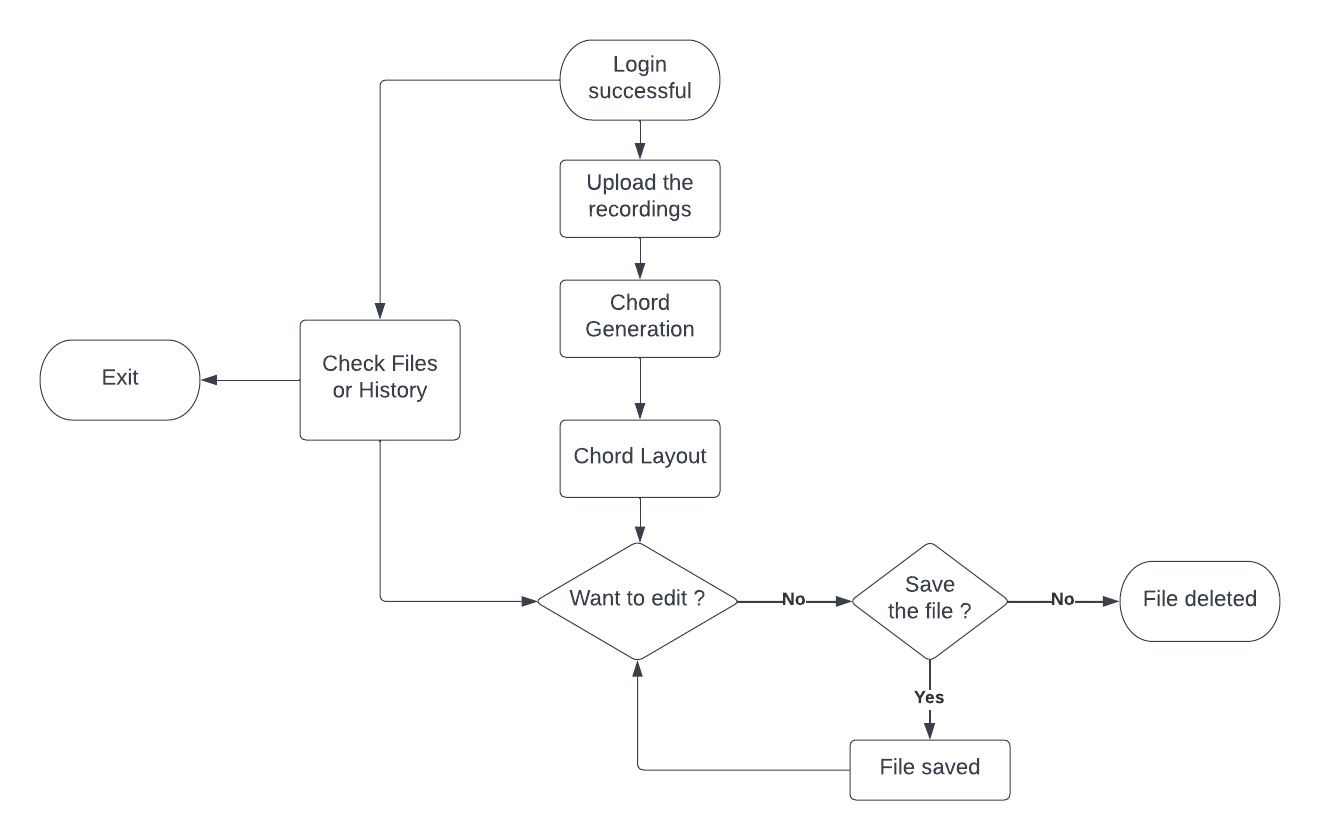
\includegraphics[scale = 0.25]{MFpage.png}
% \caption{User Flow Diagram for main function page, figure need to be improved here}
% \end{figure}


\subsection*{Main Functionality}

\begin{itemize}

\item \textbf{Sign-up and Sign-in with Email}
\\From the start, our user can sig-up with their email and then login in with our app accounts. The reason why we want our user to create an account is that we can profile our users more easily.

\item \textbf{Sign-in with with third-party Accounts}
\\ The purpose is to reduce the barriers for our users to enter our app. OAuth (Open Authorisation) is an open standard for access delegation, commonly used as a way for internet users to grant websites or applications access to their information on other websites but without giving them the passwords.This mechanism is used by companies such as Amazon, Google, Facebook, Microsoft, and Twitter to permit the users to share information about their accounts with third-party applications or websites.

\item \textbf{Ask for song tag preference}
\\After our user sign-in, a question with selective answers will show on the main page, the answers will be stored and feed to our recommendation engine, \textbf{Link to recommendation engine section}.

\item \textbf{Store and backup files on Cloud}
\\The purpose is to enable better synchronisation between devices and accessibility to the files. 
\\We will include CloudKit in our IOS design to allow users to store their saved files in iCloud, (merit: grate integration, recordings can also be stored)

\item \textbf{Recording input}
\\ 16khz

\item \textbf{Chord generation and regeneration}
\\Unlike Chordify, which generates the same chords each time for the same audio source, we provides the option for users to regenerate the chords and we aim to provides sightly different chords when regeneration button is pressed.

\item \textbf{Community Page}
\\Inspired by the Chinese music app, NetEase, one of our goals is to create a community page for our users to share their works and collaborate, 
we believe that the community element can will bring continuous traffic to our app, which can benefit the monetisation of our app in the future.
As we mentioned before, the user experience is the key factor determing the successfullness of the app design and here the quality of the posts recommended to our users is a curcial element affecting our user experience. 
Therefore, it reuqires our recommendation engine to be well designed. \autoref{Chapter6}

\item \textbf{Message Channel}
The message channel allows our users to contact each directly and share the orginal chord files 

\end{itemize}

%-----------------------------------------------------------------------------------------------------------------------------UI
\section{UI Design}
After having the map of user flow, we started to design the prototype using Figma, which is a design tool 

\begin{figure}[ht]
     \centering
     \hspace{16mm}
     \begin{subfigure}[b]{0.33\textwidth}
         \centering
         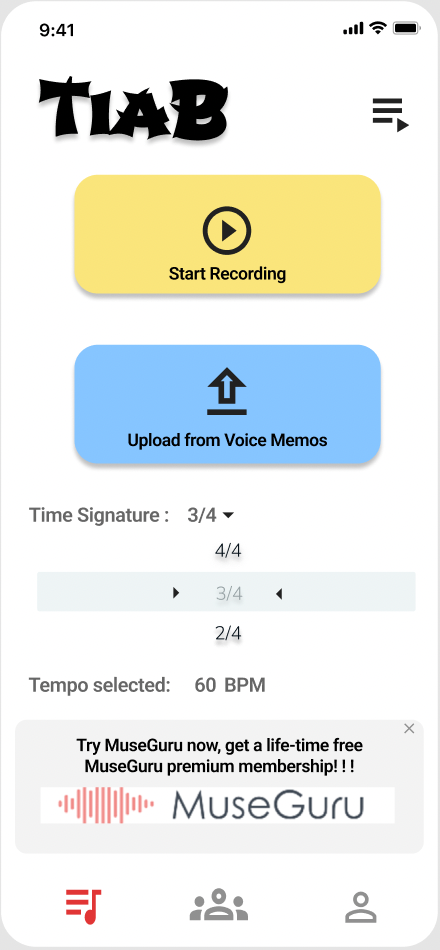
\includegraphics[width=\textwidth]{mianpage1.png}
         \caption{Log-in page}
         \label{Log-in page}
     \end{subfigure}
     \hfill
     \begin{subfigure}[b]{0.33\textwidth}
         \centering
         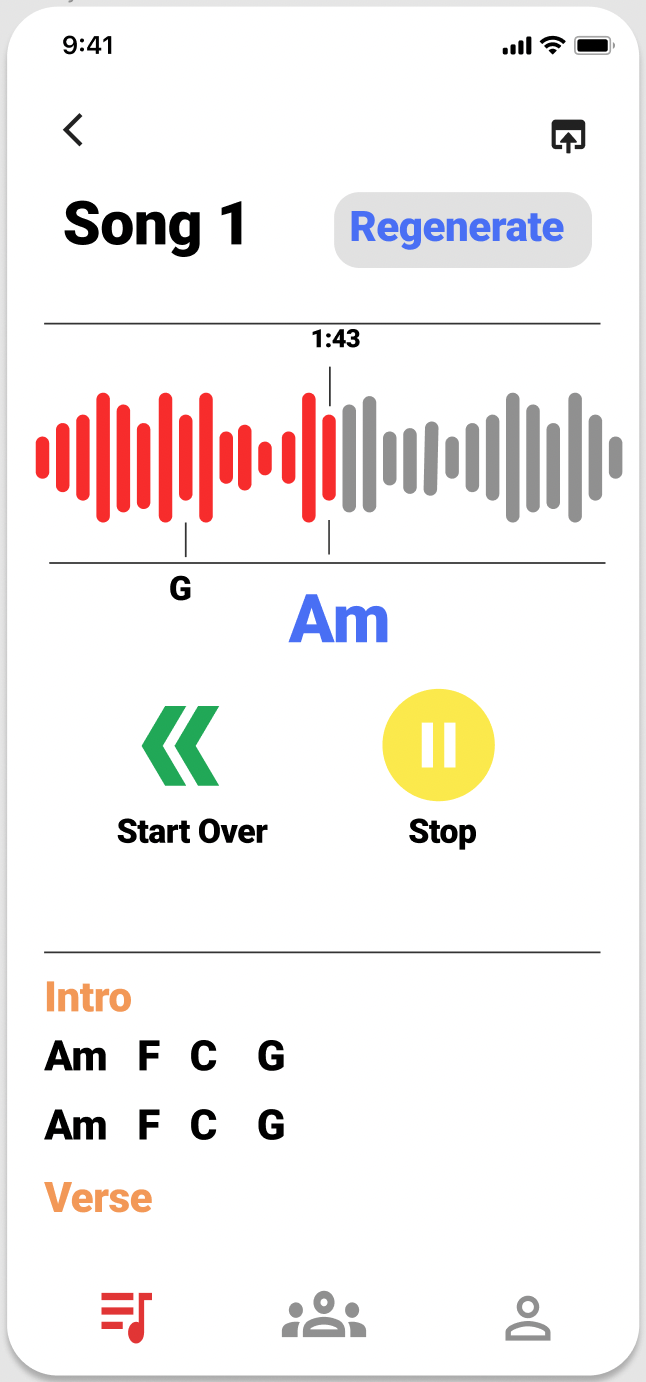
\includegraphics[width=\textwidth]{grappp.png}
         \caption{Main function page}
         \label{Main function page}
     \end{subfigure}
     \hfill
     \begin{subfigure}[b]{0.33\textwidth}
         \centering
         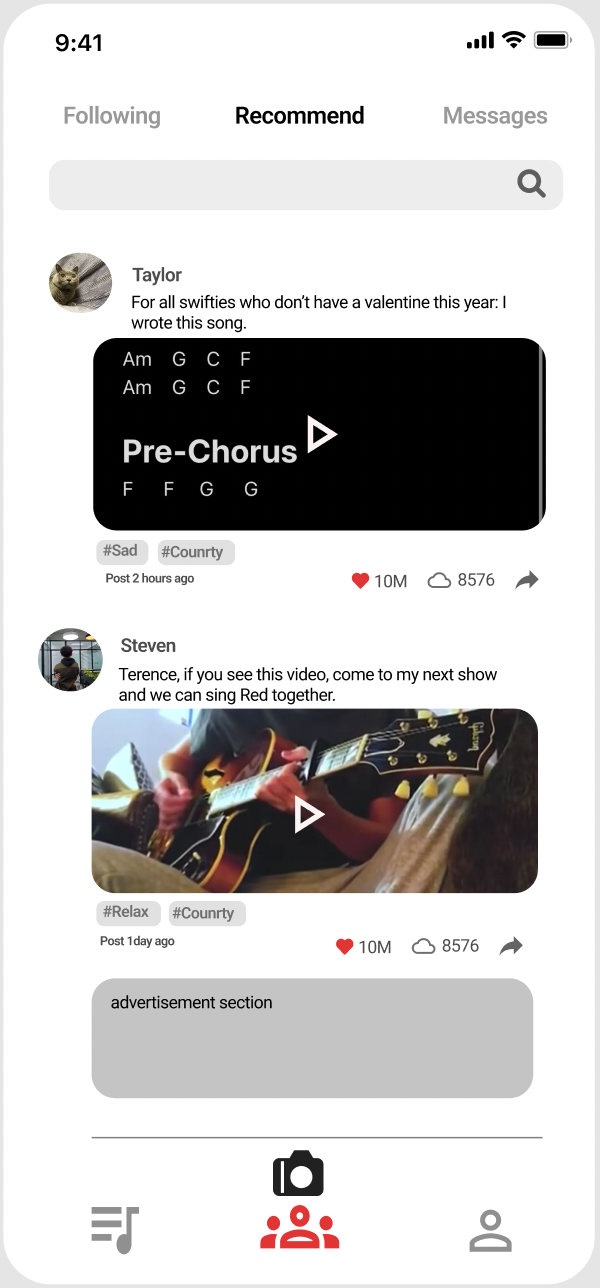
\includegraphics[width=\textwidth]{commupage.png}
         \caption{Community page}
         \label{Community page}
     \end{subfigure}
     \hspace{16mm}
        \caption{UI design for our app}
        \label{fig:three graphs}
\end{figure}

\section{Testing}
Testing stage offers us an chance to discover the problems in our current designs and 
According to Compuware, 48\% of users are less likely to use an app again if they are troubled with the app’s performance.
As reported by Compuware, only 16\% of users can give the app a try for a second or third time. \footfullcite{lowtole}

We divide testing stage into three stages, 








% Chapter Template

\chapter{Recommendation Engine}% Main chapter title
\label{Chapter6} % Change X to a consecutive number; for referencing this chapter elsewhere, use \ref{ChapterX}


The quality of recommendation system design determines the qulaity of the the posts recommended to our users. 
A recent study by Epsilon found that 90\% of consumers find personalisation appealing. Plus, a further 80\% claim they are more likely to do business with a company when offered personalised experiences.
The study also found that these consumers are 10x more likely to become VIP customers, who make more than 15 purchases per year.\footfullcite{epsilon} 
That means a well-designed recommendation system can benefit the monetisation of our app in the future.
\\Based on the types of recommendation, we can divide it into personalised and non-personalised, and personalised recommendation system can be further divided into content-based filtering system and collaborative filtering system. 
The overview of recommendation system can be seen in figure \ref{fig:overrecomm}.
\begin{figure}[ht]
\centering
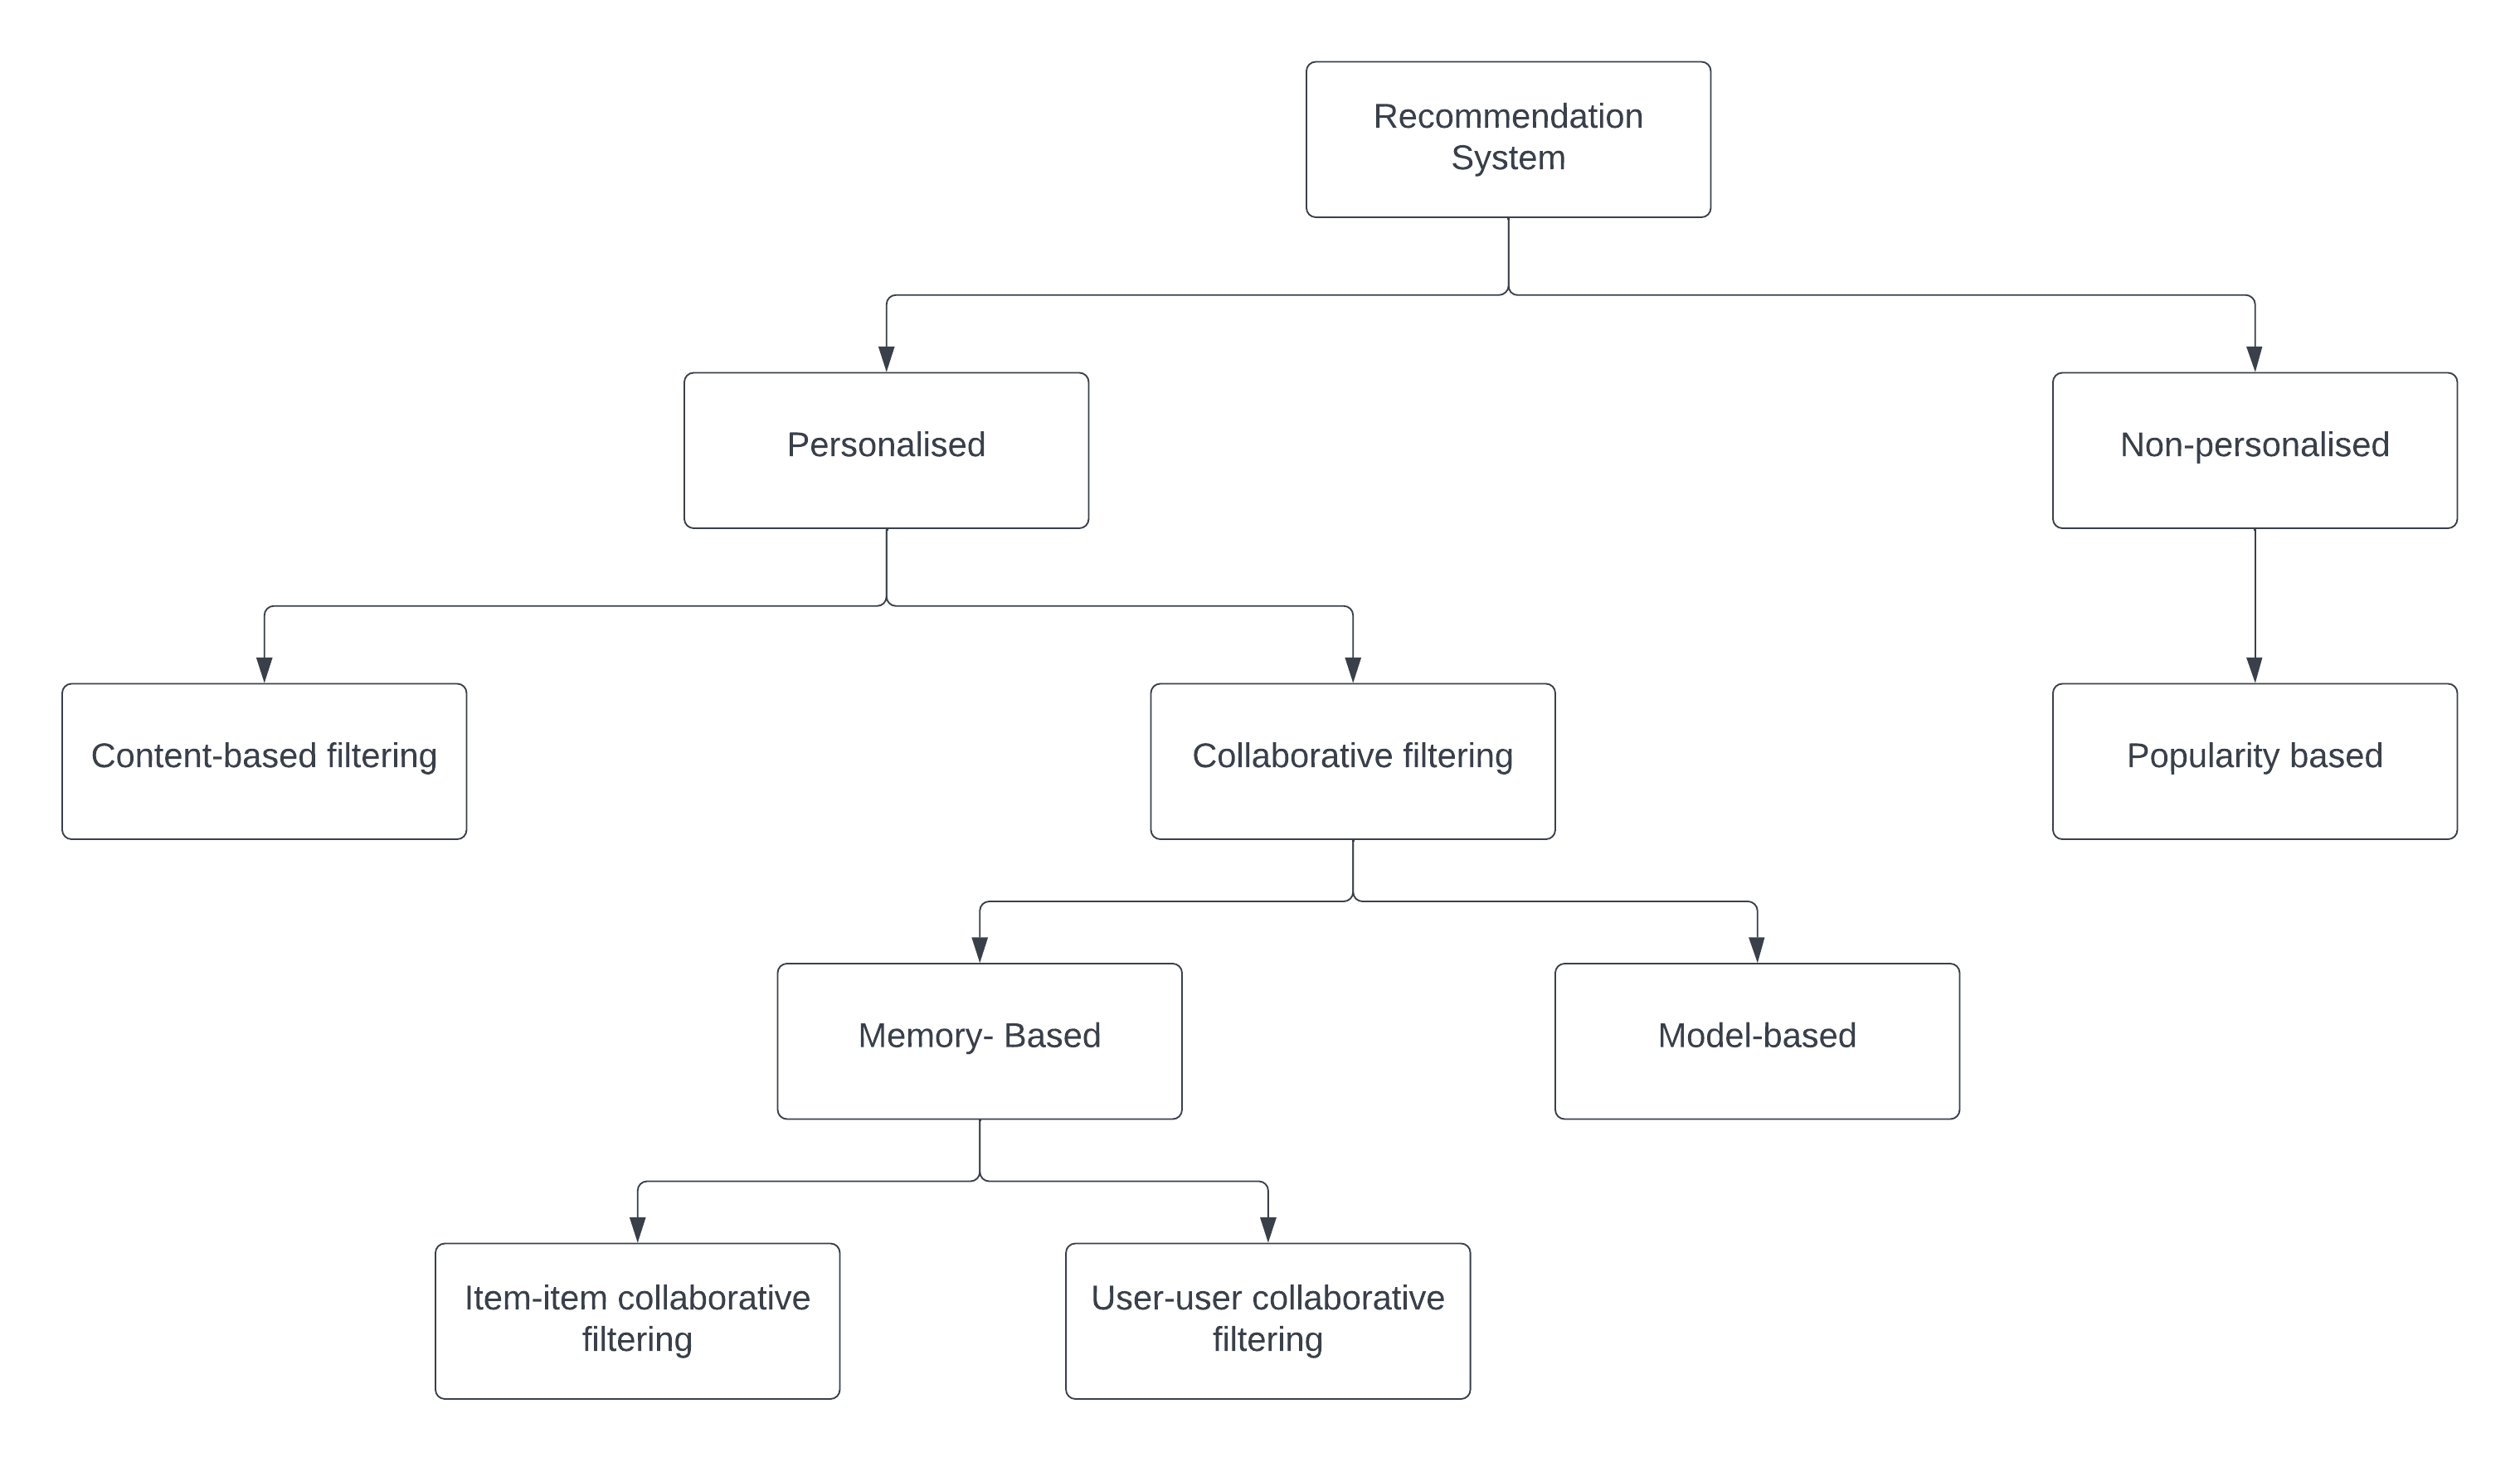
\includegraphics[scale = 0.13]{overview11.png}
\caption{Overview of recommendation system}
\label{fig:overrecomm}
\end{figure}

%-----------------------------------------------------------------------------------------------------------------------------Popularity-Based Recommendation System
\section{Popularity Based Recommendation System}
It is a type of recommendation system which works on the principle of popularity and or anything which is in trend. These systems check about the product or movie which are in trend or are most popular among the users and directly recommend those. 
Instead of recommending posts only based on the number of likes that the posts received, we can give weighting to each parameter involves in our decision and one of the weighted rating system examples is shown below.
\begin{equation}
\textbf{Rating}(v,m,R,C) = \frac{v}{v+m} \times R + \frac{m}{v+m} \times C
\end{equation}
Where:
\\$R$ is the average rating for the item.
\\$v$ is the number of votes for the item.
\\$m$ is the minimum votes required to be listed in the popular items(defined by > percentile 80 of total votes).
\\$C$ is the average rating across the whole dataset.
\\This example is used to caculate ratig scores by IMDB, which is an online database of information related to films, televison series and etc. 
Inspired by the example above, we can introduce the non-linearity in algoritms for calculate the scores of the posts to build our popularity-based recommendation system.
We want to construct $f(L,C,m,g)$, where $L$ is the number of likes the post received, $C$ is the number of comments the post received, 
$m$ is the minimum of likes to be listed as a popular item, $g$ is the gradient of change in number of likes in w.r.t time in recent period time.
\\The most obvious disadvantage of popularity based system is the non-personlisation.




%-----------------------------------------------------------------------------------------------------------------------------Content-Based Recommendation System
\section{Content Based Recommendation System}
\label{Content Based Recommendation System}
Content Based Recommendation System are based on a description of the item and a profile of the user's preferences. 
These methods are best suited to situations where there is known data on an item (name, location, description, etc.), but not on the user. 
Content-based recommenders treat recommendation as a user-specific classification problem and learn a classifier for the user's likes and dislikes based on an item's features.
\\ Before we can dive into the algorithm, we must assume that there are available features that captures the content of the item.
\\ First we need to obtain the post-feature matrix (table:\ref{itemfea}).
\begin{table}[ht]
\centering
\begin{tabular}{ |c|c|c|c|c|c|} 
 \hline
 \diagbox{Posts}{Features}&Feature1&Feature 2&Feature 3&$\cdots$&Feature $j$\\
 \hline
 Post1&&&&&\\
 \hline
 Post2&&&&&\\
 \hline
 $\vdots$&&&&&\\
 \hline
 Post $i$&&&&&\\
 \hline
 \end{tabular}
 \caption{Post Feature Matrix}
 \label{itemfea}
 \end{table}
\\The ratings given in the table measures the degree of the features in the posts, and we can assume the matrix is not sparse, which we mean the matrix is fully filled.
\\We denote that each row is the feature vector $x(i)$ for post $i$.
%
\\In addition, we need to get the profile of each individual users, which means we need to know and analyze the preference of our users, 
so we need to obtain the user parameter vector for each individual user and it reflects how the user responds to the features.
%
\\After we have post-feature matrix and user parameter vector $\theta(j)$ of user j, we apply similarity metrics, here we use cosine similarity to measure 
the resemblance bewteen $\theta(j)$ and each $x(i)$ in post-feature matrix.
\\Cosine Similarity:  As the name mentioned, It measures the cosine angle of the two vectors in the multi-dimensional space. Two things can be similar together in terms of direction rather than magnitude.
\begin{equation*}
\text{Cosine Similarity} = cos(\theta) = \frac{A \cdot B}{||A|| ||B||}
\end{equation*}
\\Our system can then recommend posts to our user$j$ based on the similarity socres.
\\The biggest problem here in our design is how can we determine the subjective features of the content, such as, genre, vibe, mood, and etc. Our current solution to this problem is including "tags" in the posts, and give limit number of choices for our users to choose from, 
and a percentage meter to indicate the degree of the features for them to set. Therefore the post-feature metrix will intensively rely on our users and it can suffer from subjectiveness.
However, we believe this design gives our users more freedom and space to show the feelings behind their songs.
\\Content based models are most advantageous for recommending items when there is an insufficient amount of rating data available. This is because other items with similar attributes might have been rated by the user. Hence, a model should be able to leverage the ratings along with the item attributes to generate recommendations even when there isn’t a lot of data.
There are some disadvantages of content-based approach as well, they are ineffective for providing recommendations for new users. 
The solution to it can be throigh an UX/UI deisgn, which is inspird by Apple Music, YouTube Music and Xiaohongshu, we would pop out a page for our users to choose preference from given choices, the bubbles will have 3 sizes to indicate 'interested in', 'like' and 'very like' levels of preferences. 
This solves the problem with the initialisation of user parameter vector. 
Another disadvantage can be that when building a model you require a history of explicit / implicit user level data for the items. It’s generally important to have a large dataset of ratings available to make robust predictions without overfitting.
\\The recommendations provided are “obvious” based on the posts / content the user has consumed. This is a disadvantage because if the user has never interacted with a particular type of post, that type will never be recommended to the user. 
For example, if the user has not seen any sad song post , then through this approach, he will never be recommended sad song posts. This is because the model is user specific and doesn’t leverage knowledge from similar users. This reduces the diversity of the recommendations, this is a negative outcome for many businesses.
\\Also people's perference will change, considering user experience, we can not ask our users to update their preference everyday or everyweek, 
and most of the time, users don't know their prefernece clearly as well. Thus being difficult to update user parameter vector is also one of the drawbacks in this approach.

%-----------------------------------------------------------------------------------------------------------------------------Collaborative Recommendation System
\section{Collaborative Filtering Recommendation System}
Collaborative filtering is the process of predicting the interests of a user by identifying preferences and information from many users. 
This is done by filtering data for information or patterns using techniques involving collaboration among multiple agents, data sources, etc. 
The underlying intuition behind collaborative filtering is that if user A and B have similar taste in a product, then A and B are likely to have similar taste in other products as well.
It has a interesting property, feature learning which is that it can learn for itself what features to use. 
\\We can divide collaborative filtering system into model-based approach and memory-based approach, and the memory-based approach can 
further be divided into item-based and user-based systems.
\\Before we dive into algorithm, we first need to construct the user-item interaction matrix \autoref{fig:UtilityM}.
\begin{table}[ht]
\centering
\begin{tabular}{ |c|c|c|c|c|c|} 
 \hline
 \diagbox{Items}{Users}&User 1&User 2&User 3&$\cdots$&User $j$\\
 \hline
 Item1&&&&&\\
 \hline
 Item2&&&&&\\
 \hline
 Item3&&&&&\\
 \hline
 $\vdots$&&&&&\\
 \hline
 Item $i$&&&&&$y^{(i,j)} \text{ if } r(i,j) = 1$\\
 \hline
 \end{tabular}
 \caption{User-Item Interaction Matrix}
 \label{fig:UtilityM}
 \end{table}
\\We denote that:
\\$r(i,j) = 1$,  if user $i$ rated item $j$ ( $0$,  otherwise.)
\\$y^{(i,j)}$ \text{is the rating by user $j$ on item $i$}
\\The first question will be faced in this approach is how we can get ratings $y^{(i,j)}$. The music posts are different from the movie rating system, considering our user experience,
we cannot ask our user to rate each post, the more sensible way is to allow them give "Like"s. However, inspired by a Chinese video-streaming app, Bilibili, we can make some changes to the "like" system. 
Instead of "like" or "not give like", we introduce a "super like" that our user can give to a post by 'press and hold' on the 'like' button .
\\Now we want to construct a rating function $y^{(i,j)}(L,t,S,T)$
\\Where
\\$L$ is 0 if "no like is given", 1 if "liked" and 2 if "super liked".
\\$t$ is the time our user spent on the post. Since we are not introducing a "dislike" feature in posts which will discourage our users to share their works,
 so we will set a threshold value for indicting "dislike". For example, if a user spends 3 seconds, below the threshold value, on a post and then exits, then the system will turn $L$ into "-1".
\\$S$ is 0 if the post has not been saved by the user and 1 if the post is saved by user.
\\$T$ is how many times the user$j$ have watched post$i$, currently.
\\Formulating the equation can be another problem, like in machine learning, we need data to fit our model or function into, which means we need to get some ratings to test or validate our rating function. 
Hence we will randomly selects small portion of posts to ask our user to rate.


%-----------------------------------------------------------------------------------------------------------------------------Memory-based CF
\subsection{Memory Based Approaches}
Memory based approaches are also often referred to as neighbourhood collaborative filtering. Essentially, ratings of user-item combinations are predicted on the basis of their neighbourhoods. 
This can be further split into user based collaborative filtering and item based collaborative filtering. 
User based essentially means that likeminded users are going to yield strong and similar recommendations. Item based collaborative filtering recommends items based on the similarity between items calculated using user ratings of those items.
\\The memory-based approach is so simple that it calculates the similarity matrix directly from the user-item matrix. There are two branches in memory based approaches, Item-based collaborative filtering and user-based collaborative filtering.

\subsubsection{Item-based Collaborative Filtering}
\\This method was first invented and used by amazon in 1998. 
Rather than matching the user to similar customers, item-to-item collaborative filtering matches each of the user’s purchased and rated items to similar items, then combines those similar items into a recommendation list. Now, let us discuss how it works.
\\Instead of applying cosine similarity, the better approah will be using pearson correlation coeffient
\\\textbf{Pearson Correlation}: The most well-known similarity metric for the linear relation is person correlation. It measures how similar two samples are based on the direction of how the value changes. 
The method for finding the similarity between two vectors is also called \textbf{Centred Cosine Similarity}. The word "Centred" means we will normalise utility matrix first by subtracting row mean, it solves the problem when we made the assumption by assuming unrated item by user will be rated 0. 
\begin{equation*}
\text{Pearson Correlation Coefficient} = \frac{\sum(x_{i} - \bar{x})(y_{i} - \bar{y})} {\sqrt{\sum(x_{i} - \bar{x})^{2} \sum{(y_{i} - \bar{y})^{2} }}}
\end{equation*}
\\We find the group of similar items based on users' similarity metric choice.
\\Select up to the top-k most similar item to recommend. \autoref{}


\subsubsection{User-based Collaborative Filtering}
\\We find the group of similar users (the group size is arbitrary) based on pearson correlation similarity metric.
\\We average the rating of each item based on the group of similar users
\\Rank the item based on the descending average rating, and recommend the target user with the item they never interacted with before.


%-----------------------------------------------------------------------------------------------------------------------------Model-based CF
\subsection{Model Based Approaches}
Model based approaches are predictive models using machine learning. Features associated to the dataset are parameterised as inputs of the model to try to solve an optimisation related problem. 
Model based approaches include using things like decision trees, rule-based approaches, latent factor models etc.
\subsubsection{Optimisation Algorithm}
\\First we need to construct the user-post iteraction matrix \autoref{fig:UtilityM}
\begin{enumerate}

\begin{table}[ht]
\centering
\begin{tabular}{ |c|c|c|c|c|c|} 
 \hline
 \diagbox{Posts}{Users}&User 1&User 2&User 3&$\cdots$&User $j$\\
 \hline
 Post1&&&&&\\
 \hline
 Post2&&&&&\\
 \hline
 Post3&&&&&\\
 \hline
 $\vdots$&&&&&\\
 \hline
 Item $i$&&&&&$y^{(i,j)} \text{ if } r(i,j) = 1$\\
 \hline
 \end{tabular}
 \caption{User-Post Interaction Matrix}
 \centering
 \end{table}

\item  Obtain a set of features folder, each measuring the degree of the content.
Denote that:
\\$r(i,j) = 1$,  if user $j$ rated item $i$ ( $0$,  otherwise.)
\\$y^{(i,j)}$ \text{is the rating by user $j$ on item $i$}
\\$\theta^{(i)}$ \text{is the parameter vector of user $j$}, which is called a latent-fatcor
\\$x^{(j)}$ \text{is the feature vector of item $i$}, which is call a latent-factor
\\$m^{(j)}$ \text{is the number of items rated by user $j$}
\\We want to reconstructed the matrix and compute the absent ratings using matrix factorisation \autoref{Matrix Factorisation}, then the predicted rate on the item $i$ by user $j$ is $(\theta^{(i)})^{T}(x^{(j)})$
\item Treat predicting the ratings of each user as a separate linear regression problem.
\item Minimise the square error term.
\end{enumerate}

Thus if we want to learn $\theta^{(i)}$ for user $j$:

\begin{equation*}
\min_{\theta^{(j)}} \frac{1}{2m^{(j)}}\sum_{i:r(i,j) = 1}\left((\theta^{(i)})^{T}x^{(j)}-y^{(i,j)}\right)^{2} + \frac{\lambda}{2m^{(j)}}\sum_{k = 1}^{n}(\theta^{(i)}_{k})^{2}
\end{equation*}
\\Where the last term is the usual regularisation term to prevent the overall equation to go to infinity and to prevent overfitting.
\\ To learn $\theta^{(1)}$,$\theta^{(2)}$, \dots, $\theta^{(j)}$:
\begin{equation*}
\min_{\theta^{(1)},\theta^{(2)}, \dots, \theta^{(j)}} \frac{1}{2}\sum_{j = 1}^{n_{u}}\sum_{i:r(i,j) = 1}\left((\theta^{(i)})^{T}x^{(j)}-y^{(i,j)}\right)^{2} + \frac{\lambda}{2}\sum_{j = 1}^{n_{u}}\sum_{k = 1}^{n}(\theta^{(i)}_{k})^{2}
\end{equation*}
where $n_{u}$ is number of users, and we get rid of term $m^{(j)}$ because it is a constant which will not affect the result when we proceed the optimisation.
\begin{equation*}
\textbf{Let     } J(\theta^{(1)},\theta^{(2)}, \dots, \theta^{(j)}) = \frac{1}{2}\sum_{j = 1}^{n_{u}}\sum_{i:r(i,j) = 1}\left((\theta^{(i)})^{T}x^{(j)}-y^{(i,j)}\right)^{2} + \frac{\lambda}{2}\sum_{j = 1}^{n_{u}}\sum_{k = 1}^{n}(\theta^{(i)}_{k})^{2}
\end{equation*}
% Then we apply \textbf{Gradient descent method}, 
% \begin{equation*}
% \\ 0 = \frac{\partial{J(\theta^{(1)},\theta^{(2)}, \dots, \theta^{(j)})}} {\partial{\theta^{(j)}}}
% \end{equation*}
\\Given $\theta^{(1)}$,$\theta^{(2)}$, \dots, $\theta^{(j)}$, to learn $x^{(i)}$:
\begin{equation*}
\min_{x^{(j)}} \frac{1}{2m^{(j)}}\sum_{j:r(i,j) = 1}\left((\theta^{(i)})^{T}x^{(j)}-y^{(i,j)}\right)^{2} + \frac{\lambda}{2m^{(j)}}\sum_{k = 1}^{n}(x^{(i)}_{k})^{2}
\end{equation*}
\\Where the last term is usual regularisation term to prevent the overall equation to go to infinity, to prevent overfitting.
\\Given $\theta^{(1)}$,$\theta^{(2)}$, \dots, $\theta^{(j)}$, to learn $x^{(1)}$,$x^{(2)}$,\dots,$x^{(i)}$:
\begin{equation*}
\min_{x^{(1)},x^{(2)}, \dots,x^{(j)}} \frac{1}{2}\sum_{i = 1}^{n_{m}}\sum_{i:r(i,j) = 1}\left((\theta^{(i)})^{T}x^{(j)}-y^{(i,j)}\right)^{2} + \frac{\lambda}{2}\sum_{j = 1}^{n_{m}}\sum_{k = 1}^{n}(\theta^{(i)}_{k})^{2}
\end{equation*}
The objective our Collaborative optimisation algorithm is that:
\\ If we are given $\theta^{(1)},\theta^{(2)}, \dots, \theta^{(j)}$, we are able to estimate $x^{(1)},x^{(2)}, \dots,x^{(i)}$
\\ If we are given $x^{(1)},x^{(2)}, \dots,x^{(i)}$, we are able to estimate $\theta^{(1)},\theta^{(2)}, \dots, \theta^{(j)}$
\\ So what we can do is that we can initialise $x^{(1)},x^{(2)}, \dots,x^{(j)}$, and then apply a \textbf{For-loop} to repeat the steps, ideally the $x^{(i)}$ and $\theta^{(j)}$ will be improved gradually. 
\\ More wisely, we can minimise $x^{(1)},x^{(2)}, \dots,x^{(i)}$ and $\theta^{(1)},\theta^{(2)}, \dots, \theta^{(j)}$ simultaneously by combining equation[] and equation[]:

\begin{equation*}
\min_{x^{(1)},x^{(2)}, \dots,x^{(n_{m})}, \theta^{(1)},\theta^{(2)}, \dots, \theta^{(n_{u})} } 
\sum_{(i,j):r(i,j) = 1}\left((\theta^{(i)})^{T}x^{(j)}-y^{(i,j)}\right)^{2} + 
\frac{\lambda}{2}
\sum_{i=1}^{n_{m}}
\sum_{k = 1}^{n}(x^{(i)})^{2}+
\frac{\lambda}{2}
\sum_{j=1}^{n_{u}}
\sum_{k = 1}^{n}(\theta^{(j)})^{2}
\end{equation*}
Finally we apply gradient descent method to solve for $x^{(1)},x^{(2)}, \dots,x^{(n_{m})}, \theta^{(1)},\theta^{(2)}, \dots, \theta^{(n_{u})}$, 
Instead of applying batch grident, which is a first-order iterative optimization algorithm for finding the minimum of a function and is expensive when the dataset is huge,
we can apply stochastic gradient descent (SGD). SGD is 
\\\textbf{Advantages}
\\The main advantage to using collaborative filtering models is its simplicity to implement and the high level coverage they provide. It is also beneficial because it captures subtle characteristics (very true for latent factor models) and does not require understanding of the item content.
\\ \textbf{Disadvantages}
\\The main disadvantage to this model is that it’s not friendly for recommending new items, this is because there has been no user/item interaction with it. This is referred to as the cold start problem. Memory based algorithms are known to perform poorly on highly sparse datasets.
\\ \textbf{Cold start problem explain}


\subsubsection{Matrix Factorisation}
\label{Matrix Factorisation}
\label{MatrixFac}
Now, instead of direct computation with the user-item interaction matrix. We will decompose the user-item interaction matrix into the latent factors matrix representing the lower-dimensional space that is more useful. The idea of decomposing is we believe that the observed user-item rating matrix is constructed from the underlying user and item latent factor matrix. Suppose we can extract the best underlying latent factor matrix that minimising the loss between the reconstructed matrix and the original matrix. 
Then we can use the inner product of the user and item latent factor matrix for inferencing an unobserved rating.It provides a better  adjustment.
\\Matrix factorisation is a class of collaborative filtering algorithms used in recommender systems. Matrix factorisation algorithms work by decomposing the user-item interaction matrix into the product of two lower dimensionality rectangular matrices.
\\There are several kinds of matrix factorisation techniques, and each of them provides a different set of results, leading to different recommendations.
\\ \textbf{TruncatedSVD with the sklearn library}
\\TruncatedSVD is a variant of the Singular Value Decomposition that calculates only the K largest singular value (n\_components). Also, It applies the linear dimensionality reduction and works well with the sparse matrix like the user-item matrix.
\\We aim to decompose the user-item matrix into these latent factors. The value of each cell will be the estimated value that satisfies the optimization constraint (SVD assumption). An example of another matrix factorization is Non-negative matrix factorization (NMF).
\\ \textbf{Funk Matrix Factorisation}
\\It reduces the user-item interaction into the lower dimensional space latent matrix. The objective of FunkFM is to estimate the latent factor matrix and the bias termed minimising the loss between the original explicit rating and the reconstructed prediction rating.
\\ Limitation: as you we see in the rating prediction, this model only takes into account the explicit rating (a true rating that the user gives to the item), and it doesn't care about the implicit rating (the number of clicks, the time spent on the item, etc.). There is an improvement about this Limitation as well. SVD++ algorithms can be further implemented to include implicit rating into consideration.
\\\textbf{Generalized Matrix Factorization(GMF)}
 \\GMF is only part of full Neural Collaborative Filtering model.
 \\The full NCF architecture has a multi-layer perception (MLP) part. This proposed idea incorporates and activates how the model can estimate the latent factors matrix with the non-linear function. The idea is that due to the complexity of the user-item interaction matrix, only the linear product of the previous matrix factorization technique is not enough to retrieve useful information. Therefore, the idea to add the MLP part to help capture the pattern in the data is proposed.


%-----------------------------------------------------------------------------------------------------------------------------Hybrid Recommendation System
\section{Hybrid Recommendation System}
Various methods of recommendations systems have their own benefits and flaws. Often, many of these methods may seem restrictive when used in isolation, especially when multiple sources of data is available for the problem. Hybrid recommender systems are ones designed to use different available data sources to generate robust inferences.
\\Hybrid recommendation systems have two predominant designs, parallel and sequential. The parallel design provides the input to multiple recommendation systems, each of those recommendations are combined to generate one output. 
The sequential design provides the input parameters to a single recommendation engine, the output is passed on to the following recommender in a sequence. Refer to the figure below for a visual representation of both designs.
% \begin{figure}[ht]
% \centering
% 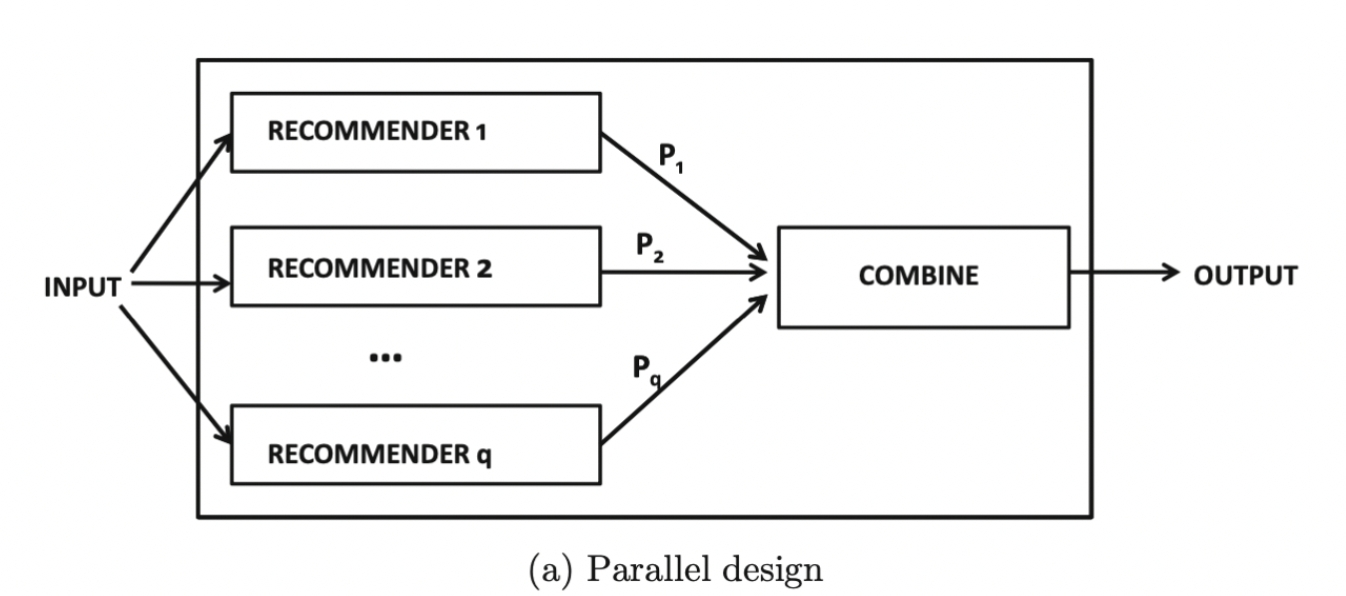
\includegraphics[scale = 0.5]{padesign}
% \caption{Parallel design of Hybrid Recommendation System}
% \centering
% \end{figure}
% \begin{figure}[ht]
% \centering
% 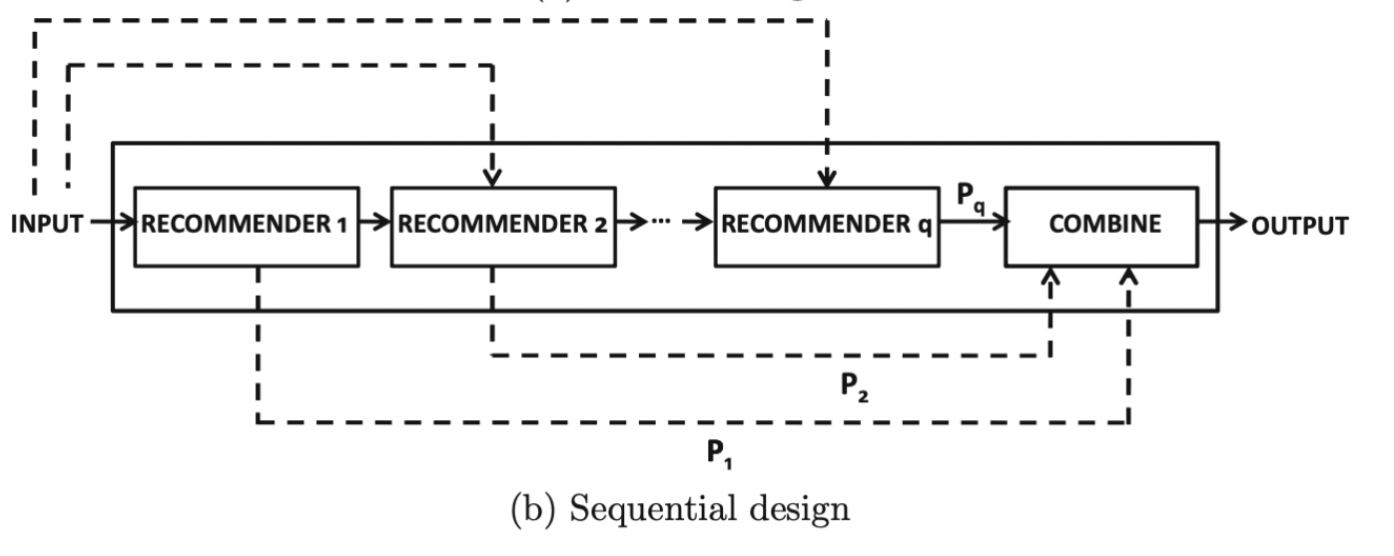
\includegraphics[scale = 0.5]{sedesign}
% \caption{Sequential design of Hybrid Recommendation System}
% \centering
% \end{figure}
\textbf{Advantages}
\\Hybrid systems combine different models to combat the disadvantages of one model with another. This overall reduces the weaknesses of using individual models and aids in generating more robust recommendations. This yields more robust and personalised recommendations for users.
\\\textbf{Disadvantages}
\\These types of models generally have high computational complexity and require a large database of ratings and other attributes to keep up to date. 
Without up to date metrics (user engagement, ratings, etc.) it makes it difficult to retrain and provide new recommendations with updated items and ratings from various users.

\section{Evaluation}
Identifying what defines a good recommendation is a problem in its self that many companies struggle with. This definition of “good” recommendations help evaluate the performance of the recommender you built. 
The quality of a recommendation can be assess through various tactics which measure coverage and accuracy. 
Accuracy is the fraction of correct recommendations out of total possible recommendations while coverage measures the fraction of objects in the search space the system is able to provide recommendations for. 
The method of evaluation of a recommendation is solely dependent on the dataset and approach used to generate the recommendation. 
Recommender systems share several conceptual similarities with the classification and regression modelling problem. 
In an ideal situation, we would want to see how real users react to recommendations and track metrics around the user to improve your recommendation, however, this is quite difficult to accomplish. 
Common statistical accuracy measures to evaluate accuracy of a recommender are RMSD, MAE, and k fold cross validation.

\subsection{K Fold Cross Validation}
This is one of the non-exhaustive validation methods, which means it does not compute all ways of splitting the original sample.
\begin{itemize}
\item Imagine you’ve built a model which will predict how well a user will rate an item based on a set of features. K fold cross validation can be used to infer the results of the model through accuracy metrics
\item Same idea as a train test split, except we create K many randomly assigned training and test sets
\item Each individual training set / fold is used to train on the recommendation system independently and then measure the accuracy of the resulting systems against the test set
\item We take the average of accuracy score to see how well the recommendation system is learning
\item This method is beneficial to prevent your model from overfitting, however it is a computationally extensive process
\end{itemize}

\subsection{Mean Absolute Error (MAE)}
Mean absolute error represents the average absolute value of each error in rating prediction
\begin{equation*}
\text{MAE} = \frac{\sum^{i=n}_{i=1}|y_{i} - x_{i}|}{n}
\end{equation*}
$y_{i}  = $ prediction
\\$x_{i}  = $ True Value
\\$n$ = total number of data points
\\Lower the MAE score the better.

\subsection{Root Mean Square Deviation(RMSD)}
\begin{equation*}
\text{RMSD} = \sqrt{\frac{\sum^{i=N}_{i=1}(y_{i} - x_{i})^{2}}{N}}
\end{equation*}

\begin{itemize}
\item A similar metric to MAE but has a stronger penalty for when the prediction is very far from the true value and weaker penalty for when the prediction is closer to the true value
\item Taking the squares off the difference of true and predicted values instead of the sum of the absolute values. This ensures that the resulting value is always positive and is larger when the difference is high and smaller when the difference is low.
\item The lower the RMSD score the better
\end{itemize}


\section{Implementation}
\subsection{System Design}
We finally decided to design our recommendation system using a hybrid system shown in \autoref{hybridd}. The system consists four sub-systems in parallel with each other, 
with one of the sub-systems is built with content-based and model-based filtering connected in series.
\begin{figure}[ht]
    \centering
    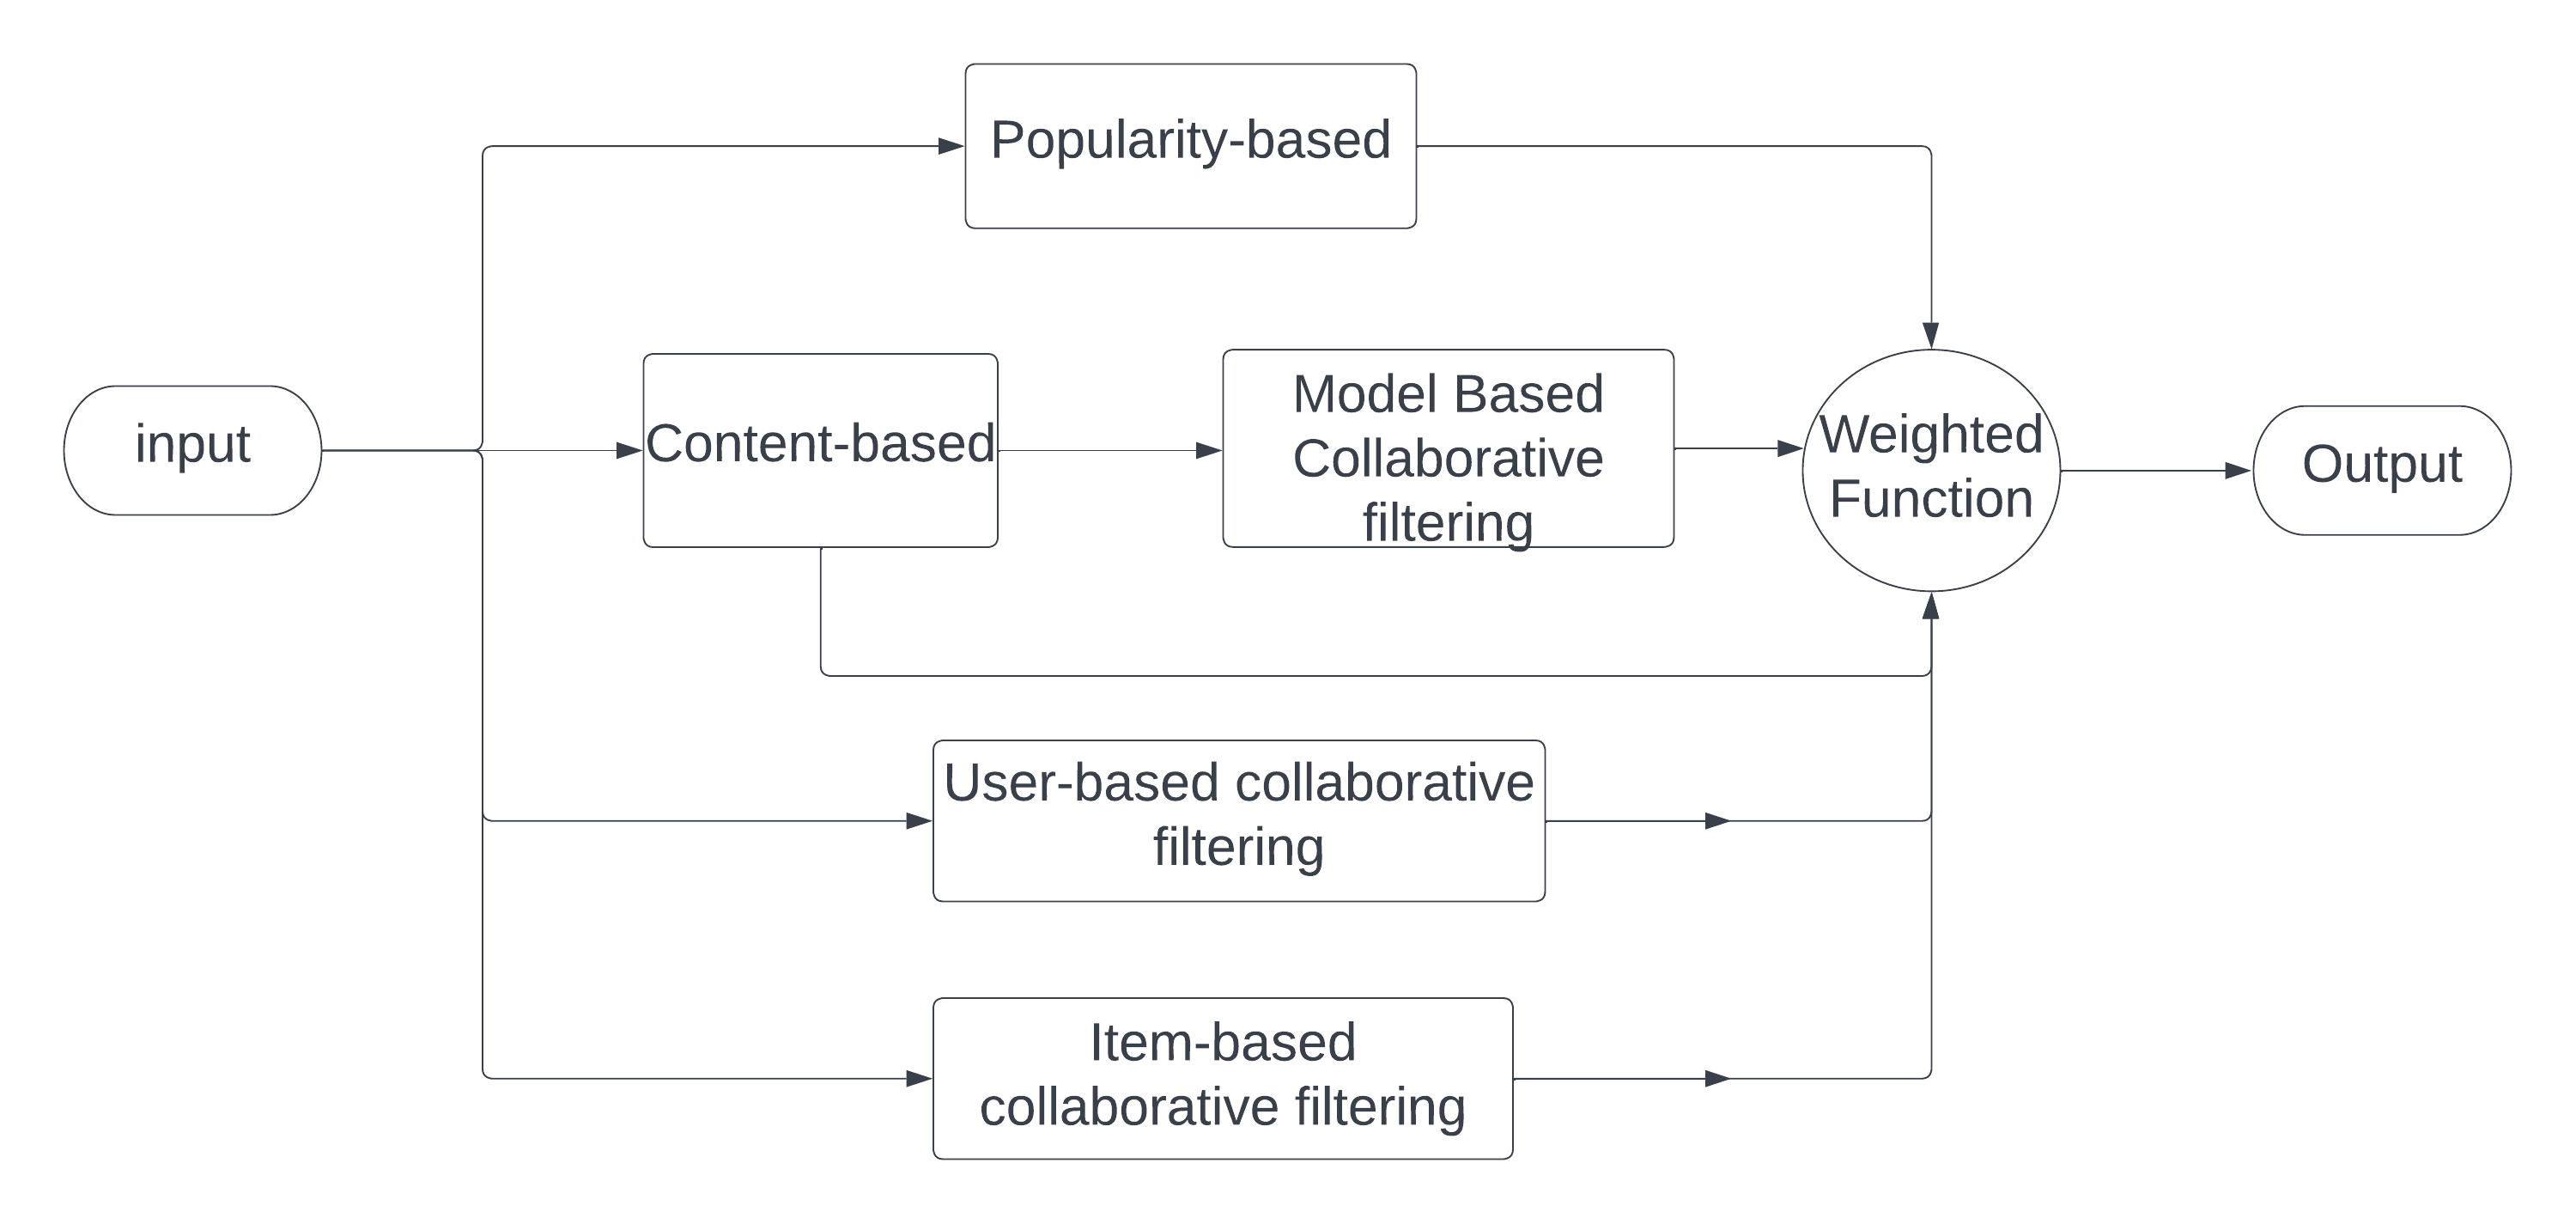
\includegraphics[scale = 0.15]{hybridd.png}
    \caption{Hybrid recommendation system design}
    \label{hybridd}
    \end{figure}
\\Firstly, the input which is information gathered from our users, will be passed through the popularity based system to get the ratings for their popularity.
\\In addition, the input will be feed into content-based system to have ratings based on the similarity between users' perference and posts' features. 
The reason why we also pass the output after the content-based system through a model-based collaborative filtering is to solve the limitations in last step, 
which are that users parameters vector can not be updated and users will not be recommended the type of posts if they have not interact with it before.
\\Furthermore, the input will pass through the user-based and item-based collaborative filtering system in parallel with other systems, 
to have the ratings of posts based on the analysis of group behaviors.
\\Finally after we have ratings after each system, we pass all the results into a weighting function, where we give weights to each sub-system output, and then apply a linear combination.
The weights coefficients are calculated based on the performance and reliability of the sub-systems.

\subsection{Top-k Recommendation}
\label{Top-k Recommendation}
In reality, we only care about the top-rated posts for our users. 
\\top-k explained here




 

% Chapter Template
\chapter{Audio Processing} % Main chapter title

\label{Chapter5} % Change X to a consecutive number; for referencing this chapter elsewhere, use \ref{ChapterX}
Before we feed the audio clip to our machine learning model, it is crucial to pre-process the signal as to achieve higher accuracy
and avoid further deterioration.
The choice and implementation of noise filter will then be explained in \autoref{sec:NF}. We then feed the filtered output 
to a pitch detection algorithm (PDA) in \autoref{sec:PDA} and then a key detection algorithm (KDA) in \autoref{sec:KDA}
Figure \ref{flowchart} shows the flowchart of the audio processing part of our project.

\begin{figure}[h]
	\centering
	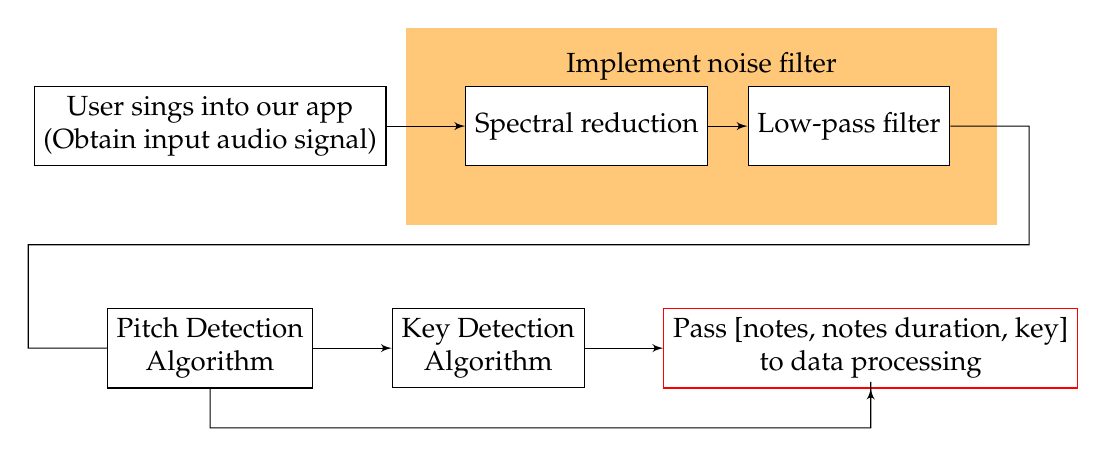
\begin{tikzpicture}[>=latex']
		\tikzset{
			block/.style= {draw, rectangle, fill=white, align=center,minimum width=2cm,minimum height=1cm},
			fbox/.style = {rectangle, draw, densely dashed, inner sep=4mm},
			input/.style={ % requires library shapes.geometric
			draw,
			trapezium,
			trapezium left angle=60,
			trapezium right angle=120,
			minimum width=2cm,
			align=center,
			minimum height=1cm},
		}
		
		%nodes
		\node (n1) [block]  {User sings into our app\\ 
					(Obtain input audio signal)}; 
		%beige bg
		\node (bg) [right= 4cm of n1, anchor=center, draw=none, fill={rgb:orange,1;yellow,2;pink,5}, minimum width=7.5cm,minimum height=2.5cm]{};
		\node (bglabel) [above = -0.8cm of bg]{Implement noise filter};
		
		\node (n2) [block, right=1cm of n1]
					{Spectral reduction};
		\node (n3) [block, right=0.5cm of n2]
					{Low-pass filter};
		\node (n4) [block, below=1.8cm of n1] 
					{Pitch Detection\\ Algorithm};
		\node (n5) [block, right=1cm of n4] 
					{Key Detection\\ Algorithm};
		\node (n6) [block, draw=red, right=1cm of n5]
					{Pass [notes, notes duration, key]\\
					to data processing};
		\node [coordinate, below right =1cm and 1cm of n3] (right1) {};  %% Coordinate on right and middle
		\node [coordinate, above left =0.8cm and 1cm of n4] (left1) {};  %% Coordinate on left and middle

		\node [coordinate, below =0.5cm of n4] (n4coor) {};  %% Coordinate on right and middle
		\node [coordinate, below =0.5cm of n6] (n6coor) {};  %% Coordinate on left and middle
		\path[draw,->]   (n1) edge (n2)
					(n2) edge (n3)
					(n3) -| (right1) -- (left1) |-  (n4)
					(n4) edge (n5)
					(n4.south) -| (n4coor) -- (n6coor) |-  (n6.south)
					(n5) edge (n6);

	\end{tikzpicture}
	\caption{Flowchart of audio processing}
	\label{flowchart}
\end{figure}

%----------------------------------------------------------------------------------------
%	SECTION 0
%----------------------------------------------------------------------------------------
\section{Assumptions}
Before we delineate the approach to audio processing, there are some assumptions that our model
is built on:
\begin{itemize}
	\item \textbf{Assumption 1:} Users' audio input device does not contain active noise cancelling functions.
	\item \textbf{Assumption 2:} Users do not sing with the technique of polyphonic overtone singing.
	\item \textbf{Assumption 3:} Signal and noise are uncorrelated.
	\item \textbf{Assumption 4:} Noise is a stationary or slowly varying process.
	\item \textbf{Assumption 5:} Noise spectrum does not change drastically during the recording.
\end{itemize}

%----------------------------------------------------------------------------------------
%	SECTION 1
%----------------------------------------------------------------------------------------
\section{Noise Filter}
\label{sec:NF}
Noise filtering is essential as it reduces or eliminates the noise present in the input signal.
A conventional method to quantify noise is to use the signal-to-noise ratio (SNR), which is often 
represented in decibels.
\[SNR=10*log_{10}\frac{P_{signal}}{P_{noise}}\]
As its name suggests, SNR is the power ratio between the desired signal and undesired noise. Effectively,
we would like to use noise filters to achieve a higher SNR.\\ 
There are a few sources of noise when a user records himself with a microphone.
Firstly, there exists self-noise, which is the instrument noise produced by the microphone itself.
Noise may be induced or created when the signal passes through electronic components like transistors 
and printed circuit boards\footfullcite{selfnoise}.
The second source, ambient noise, contributes to a large portion of noise present in a recording.
Room reflections, extraneous noise, electromagnetic interference and mechanical noise are some causes 
of ambient noise.  

%-----------------------------------
%	SUBSECTION 1
%-----------------------------------
\subsection{Possible Models}
Most of the noise filters work in the frequency and spectral domain, here we are going to inspect and
compare three noise reduction mechanisms.

\begin{enumerate}
	\item Low-pass filter (LPF)\\
	LPF passes signals with frequency \(f<f_{c}\), where \(f_{c}\) is the cut-off frequency, and attenuates
	signals with \(f>f_{c}\). 
	In order to implement an LPF, we have to transform the signal from time domain to 
	frequency domain using Fourier Transform (FT). An ideal LPF would completely remove frequencies that are
	higher than \(f_{c}\) and is a non-casual linear time-invariant system. 
	\[H(f) = rect(\frac{f}{2B})\]
	\[h(t))= \mathfrak{F}^{-1}{H(f)} = \int_{-B}^{B} e^{2(\pi)ift}\,df = 2Bsinc(2Bt)\]
	The impulse response of an LPF is a sinc function that extends to [-$\infty$,$\infty$]. This is why it is 
	impossible to realize an ideal LPF since that will take infinite time and memory.
	%LPF avoids aliasing since it removes the high-frequency content but not the desired signal why is this sentence here%

	\item Wavelet transform\\
	Wavelet transform creates a representation of the signal in both time and frequency domain so localized 
	information of the signal can be efficiently accessed. It is often compared with FT, which
	has the following limitations: 
	\begin{enumerate}
		\item For windowed FT, if the feature is larger or shorter than the window, it cannot be captured completely.
		\item Time resolution for high frequencies is the same for low frequencies. As frequency increases, rate of 
		change of the signal increases, and high frequency signals contain more information in a window than that of 
		low frequency, thus we need a higher time resolution for that.
	\end{enumerate}
	Wavelet transform analyzes a signal by its different frequency components at multiple resolution so features that are 
	undiscovered at one resolution may be obvious at another. There are mainly 2 types of wavelet transforms, namely 
	continuous wavelet transform (CWT) and discrete wavelet transform (DWT).
	
	CWT finds how alike a wavelet is in a signal, given the dilation and translation parameter of the wavelet\footfullcite{wavelet}. 
	This can be found by convolving the mother wavelet with our signal.

	\begin{equation*} 
		\text{CWT}(\mathrm{a},\mathrm{b}; \mathrm{x}(\mathrm{t}),\psi(\mathrm{t}))=\int_{-\infty}^{\infty}[\mathrm{x}(\mathrm{t})\frac{1}{\mathrm{a}}-\psi^{*}(\frac{\mathrm{t}-\mathrm{b}}{\mathrm{a}})]\text{dt}
	\end{equation*}

	where $x(t)$ is the original signal, $\psi(t)$ is the mother wavelet, $a$ is a dilation parameter and $b$ is a translation parameter\footfullcite{wavelet_denoise}.
	Dilation factor represents how dispersed the wavelet is (similar to scaling) while translation factor tells us where the wavelet is
	positioned in time (similar to shifting). 
	
	\begin{figure}
		\centering
		\begin{subfigure}{.4\textwidth}
		  \centering
		  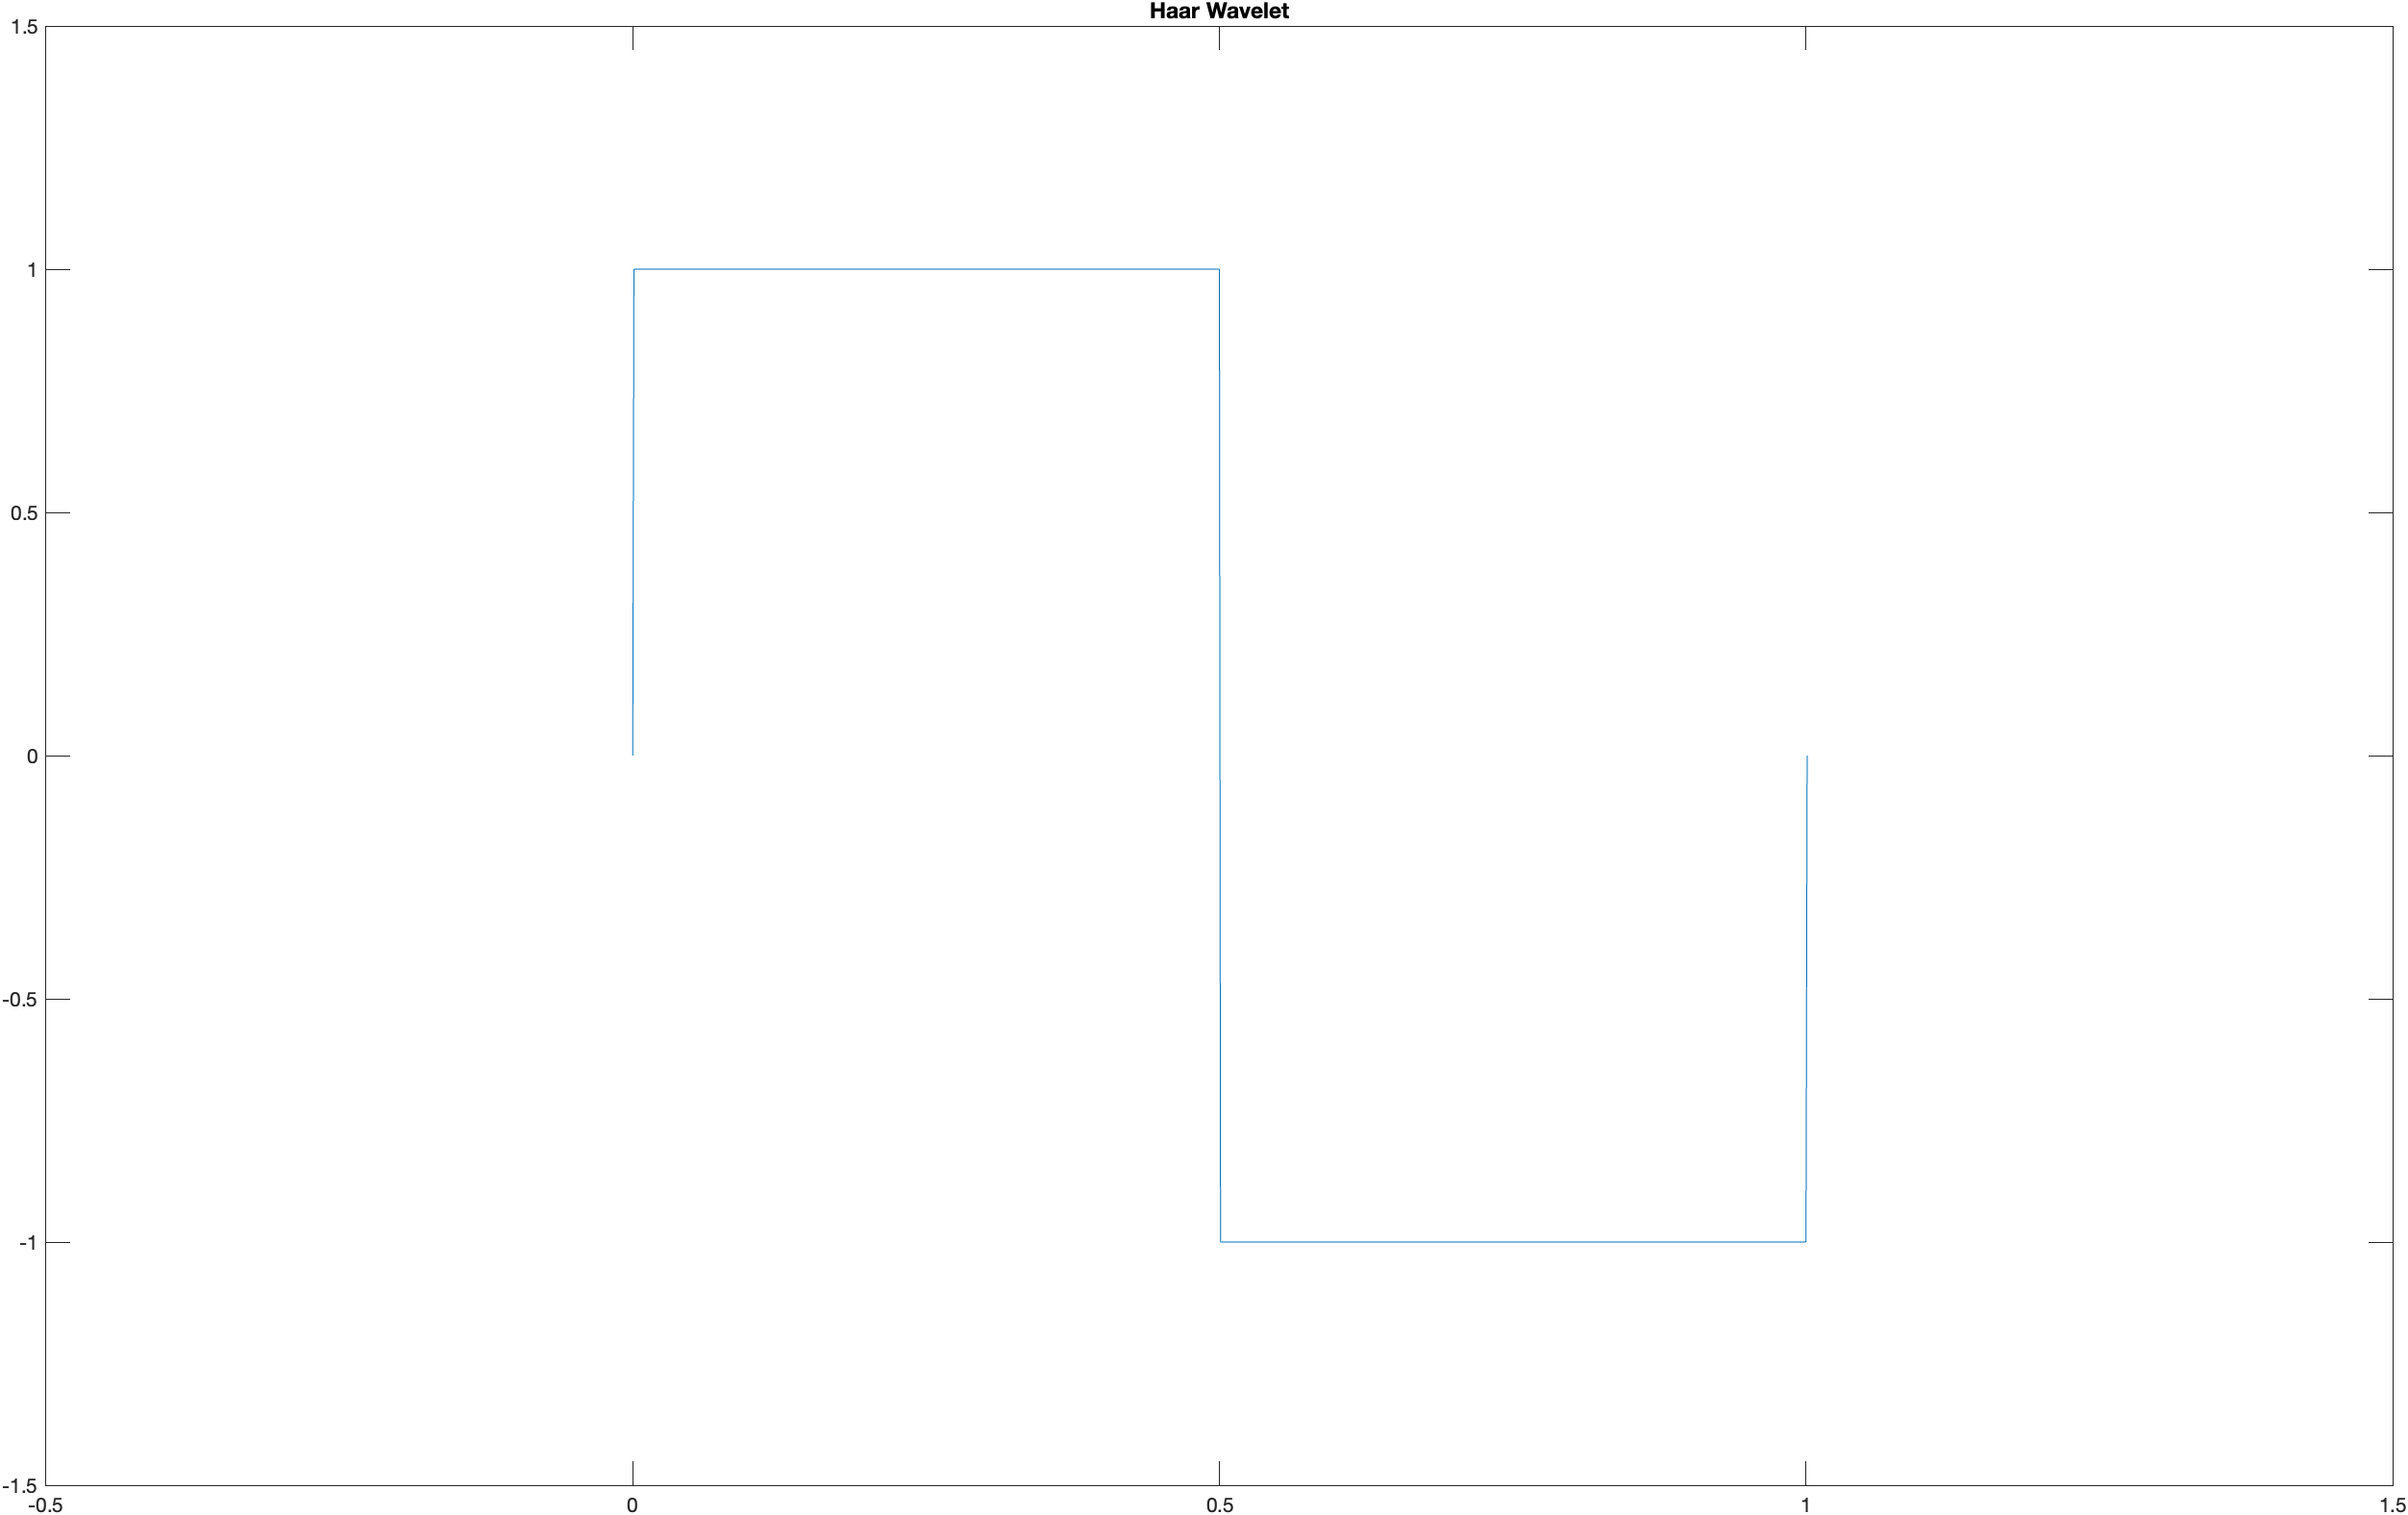
\includegraphics[width=\linewidth]{haar.png}
		  \caption{Haar wavelet}
		  \label{Haar}
		\end{subfigure}
		\hfill
		\begin{subfigure}{.4\textwidth}
			\centering
			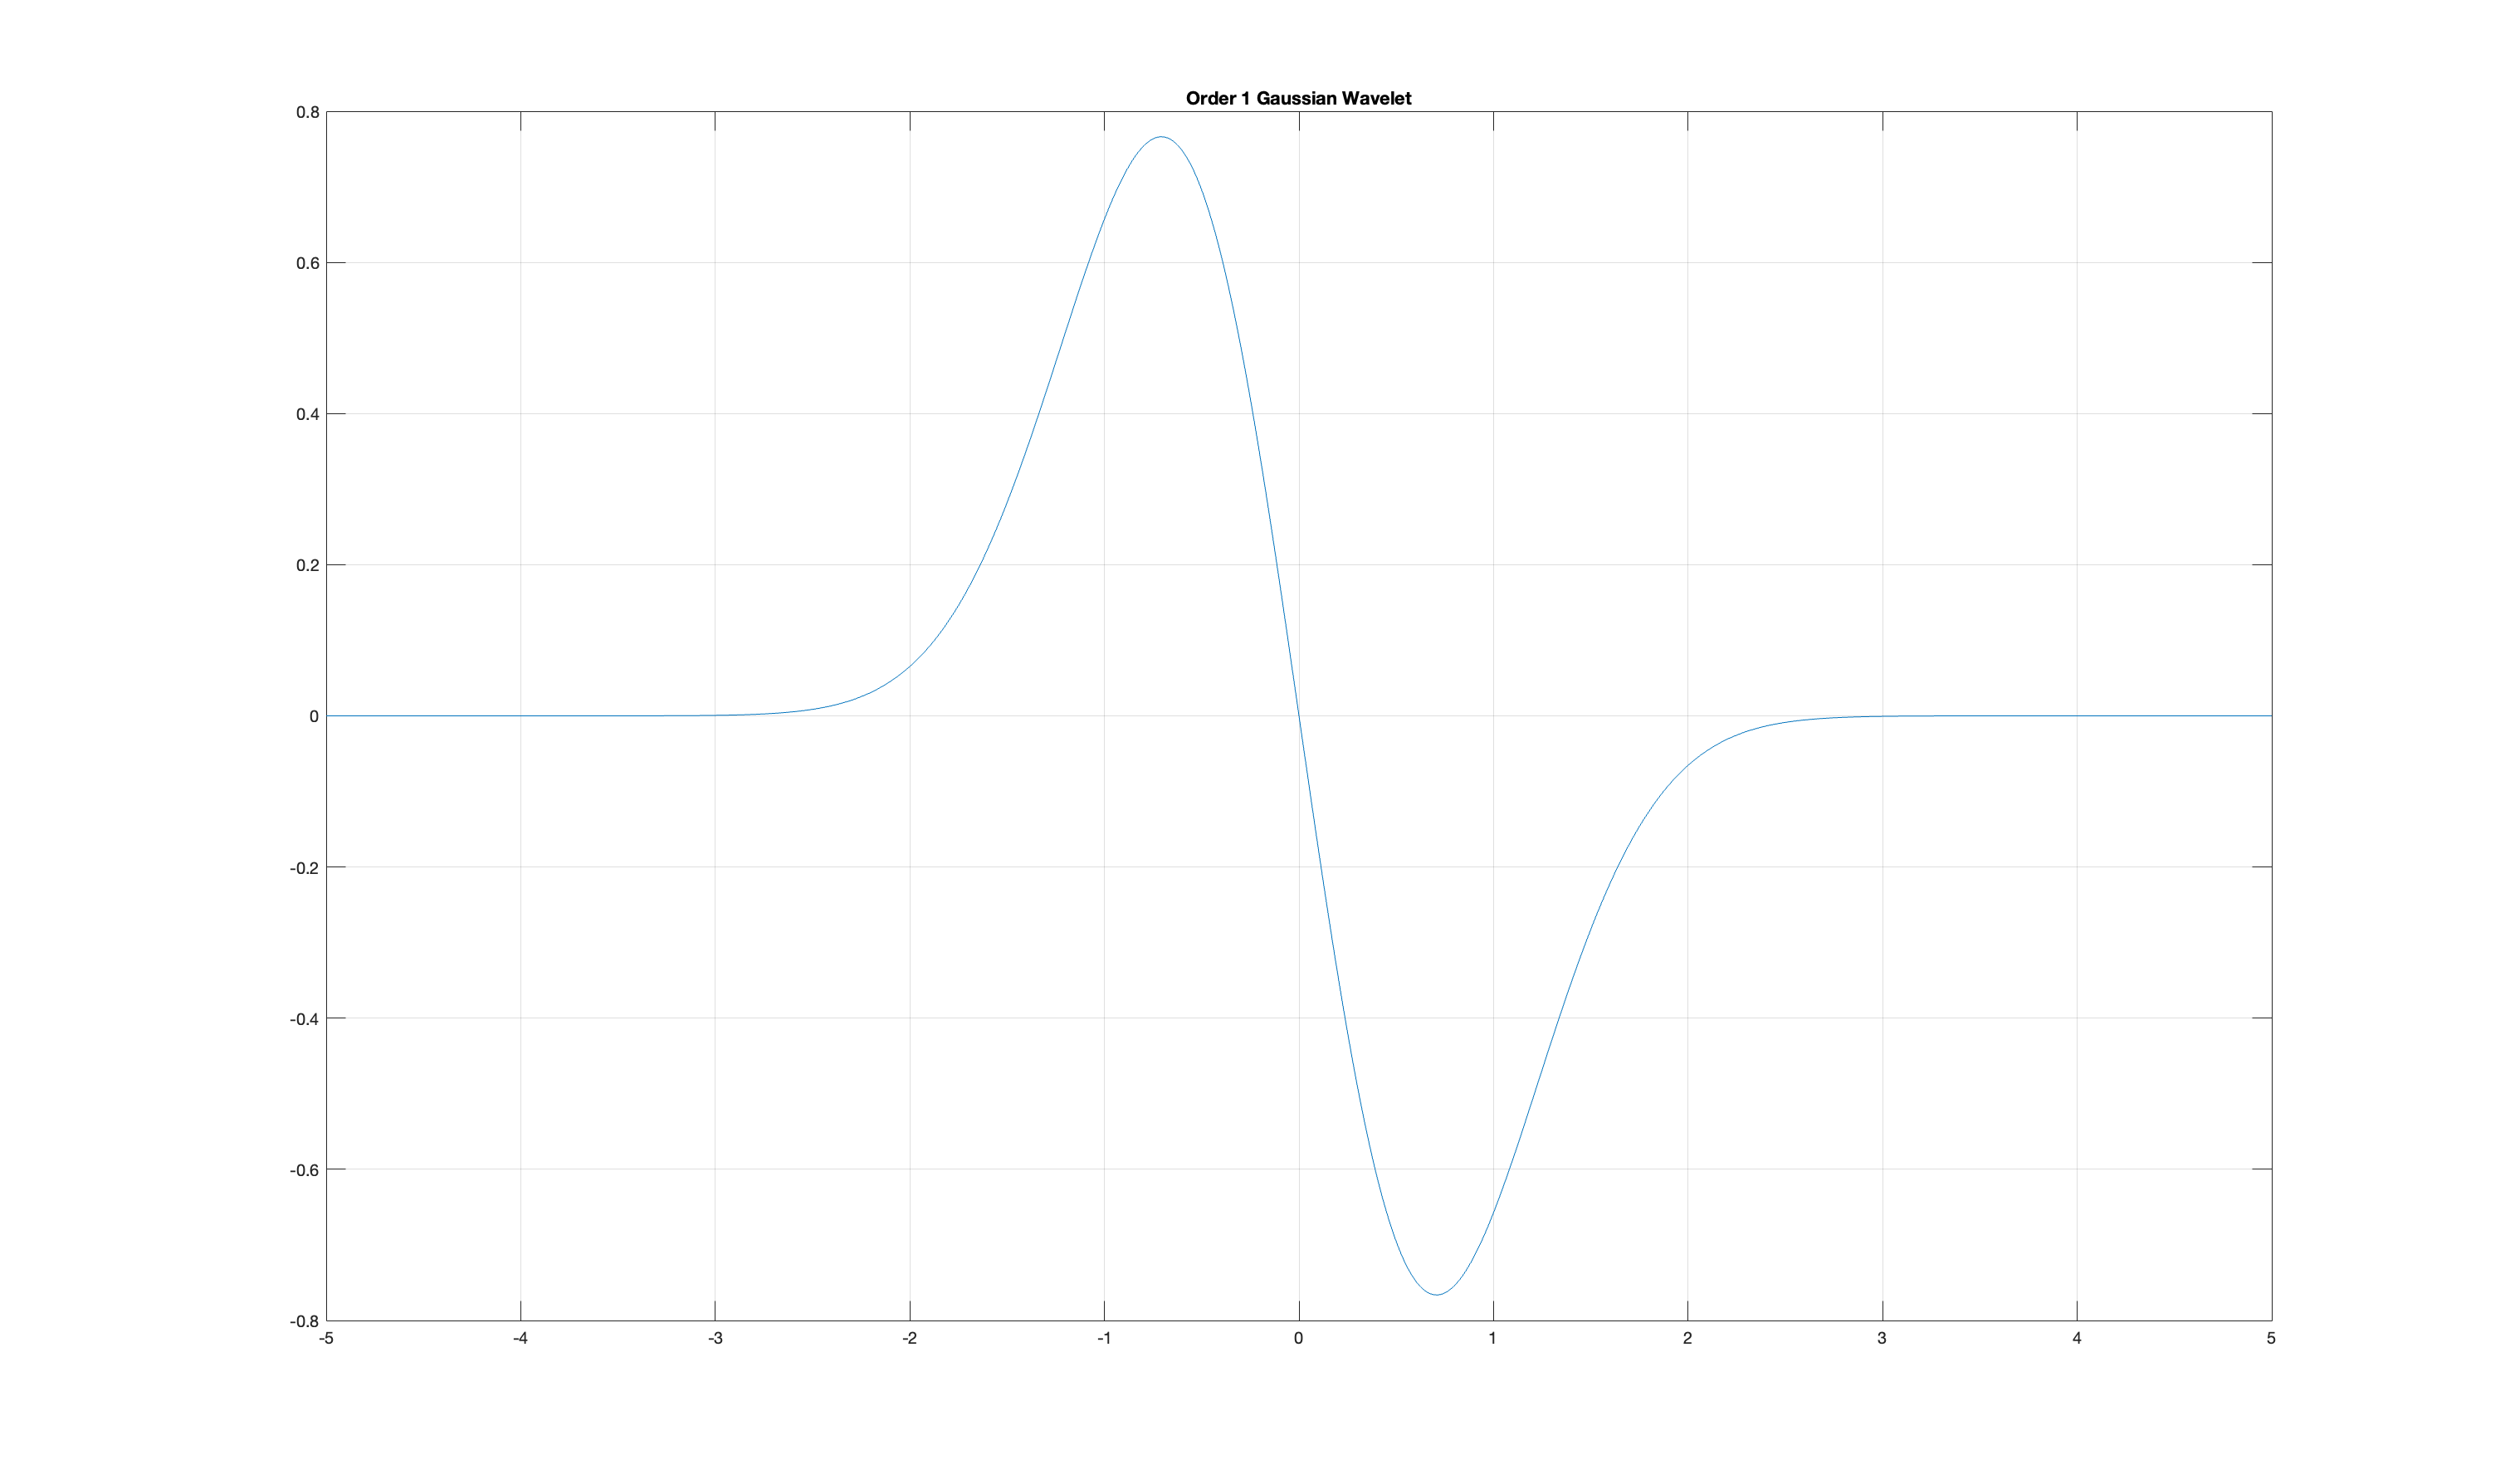
\includegraphics[width=\linewidth]{order1gaussian.png}
			\caption{Gaussian wavelet \\of order 1}
			\label{order1}
		\end{subfigure}
		\hfill
		\begin{subfigure}{.4\textwidth}
		  \centering
		  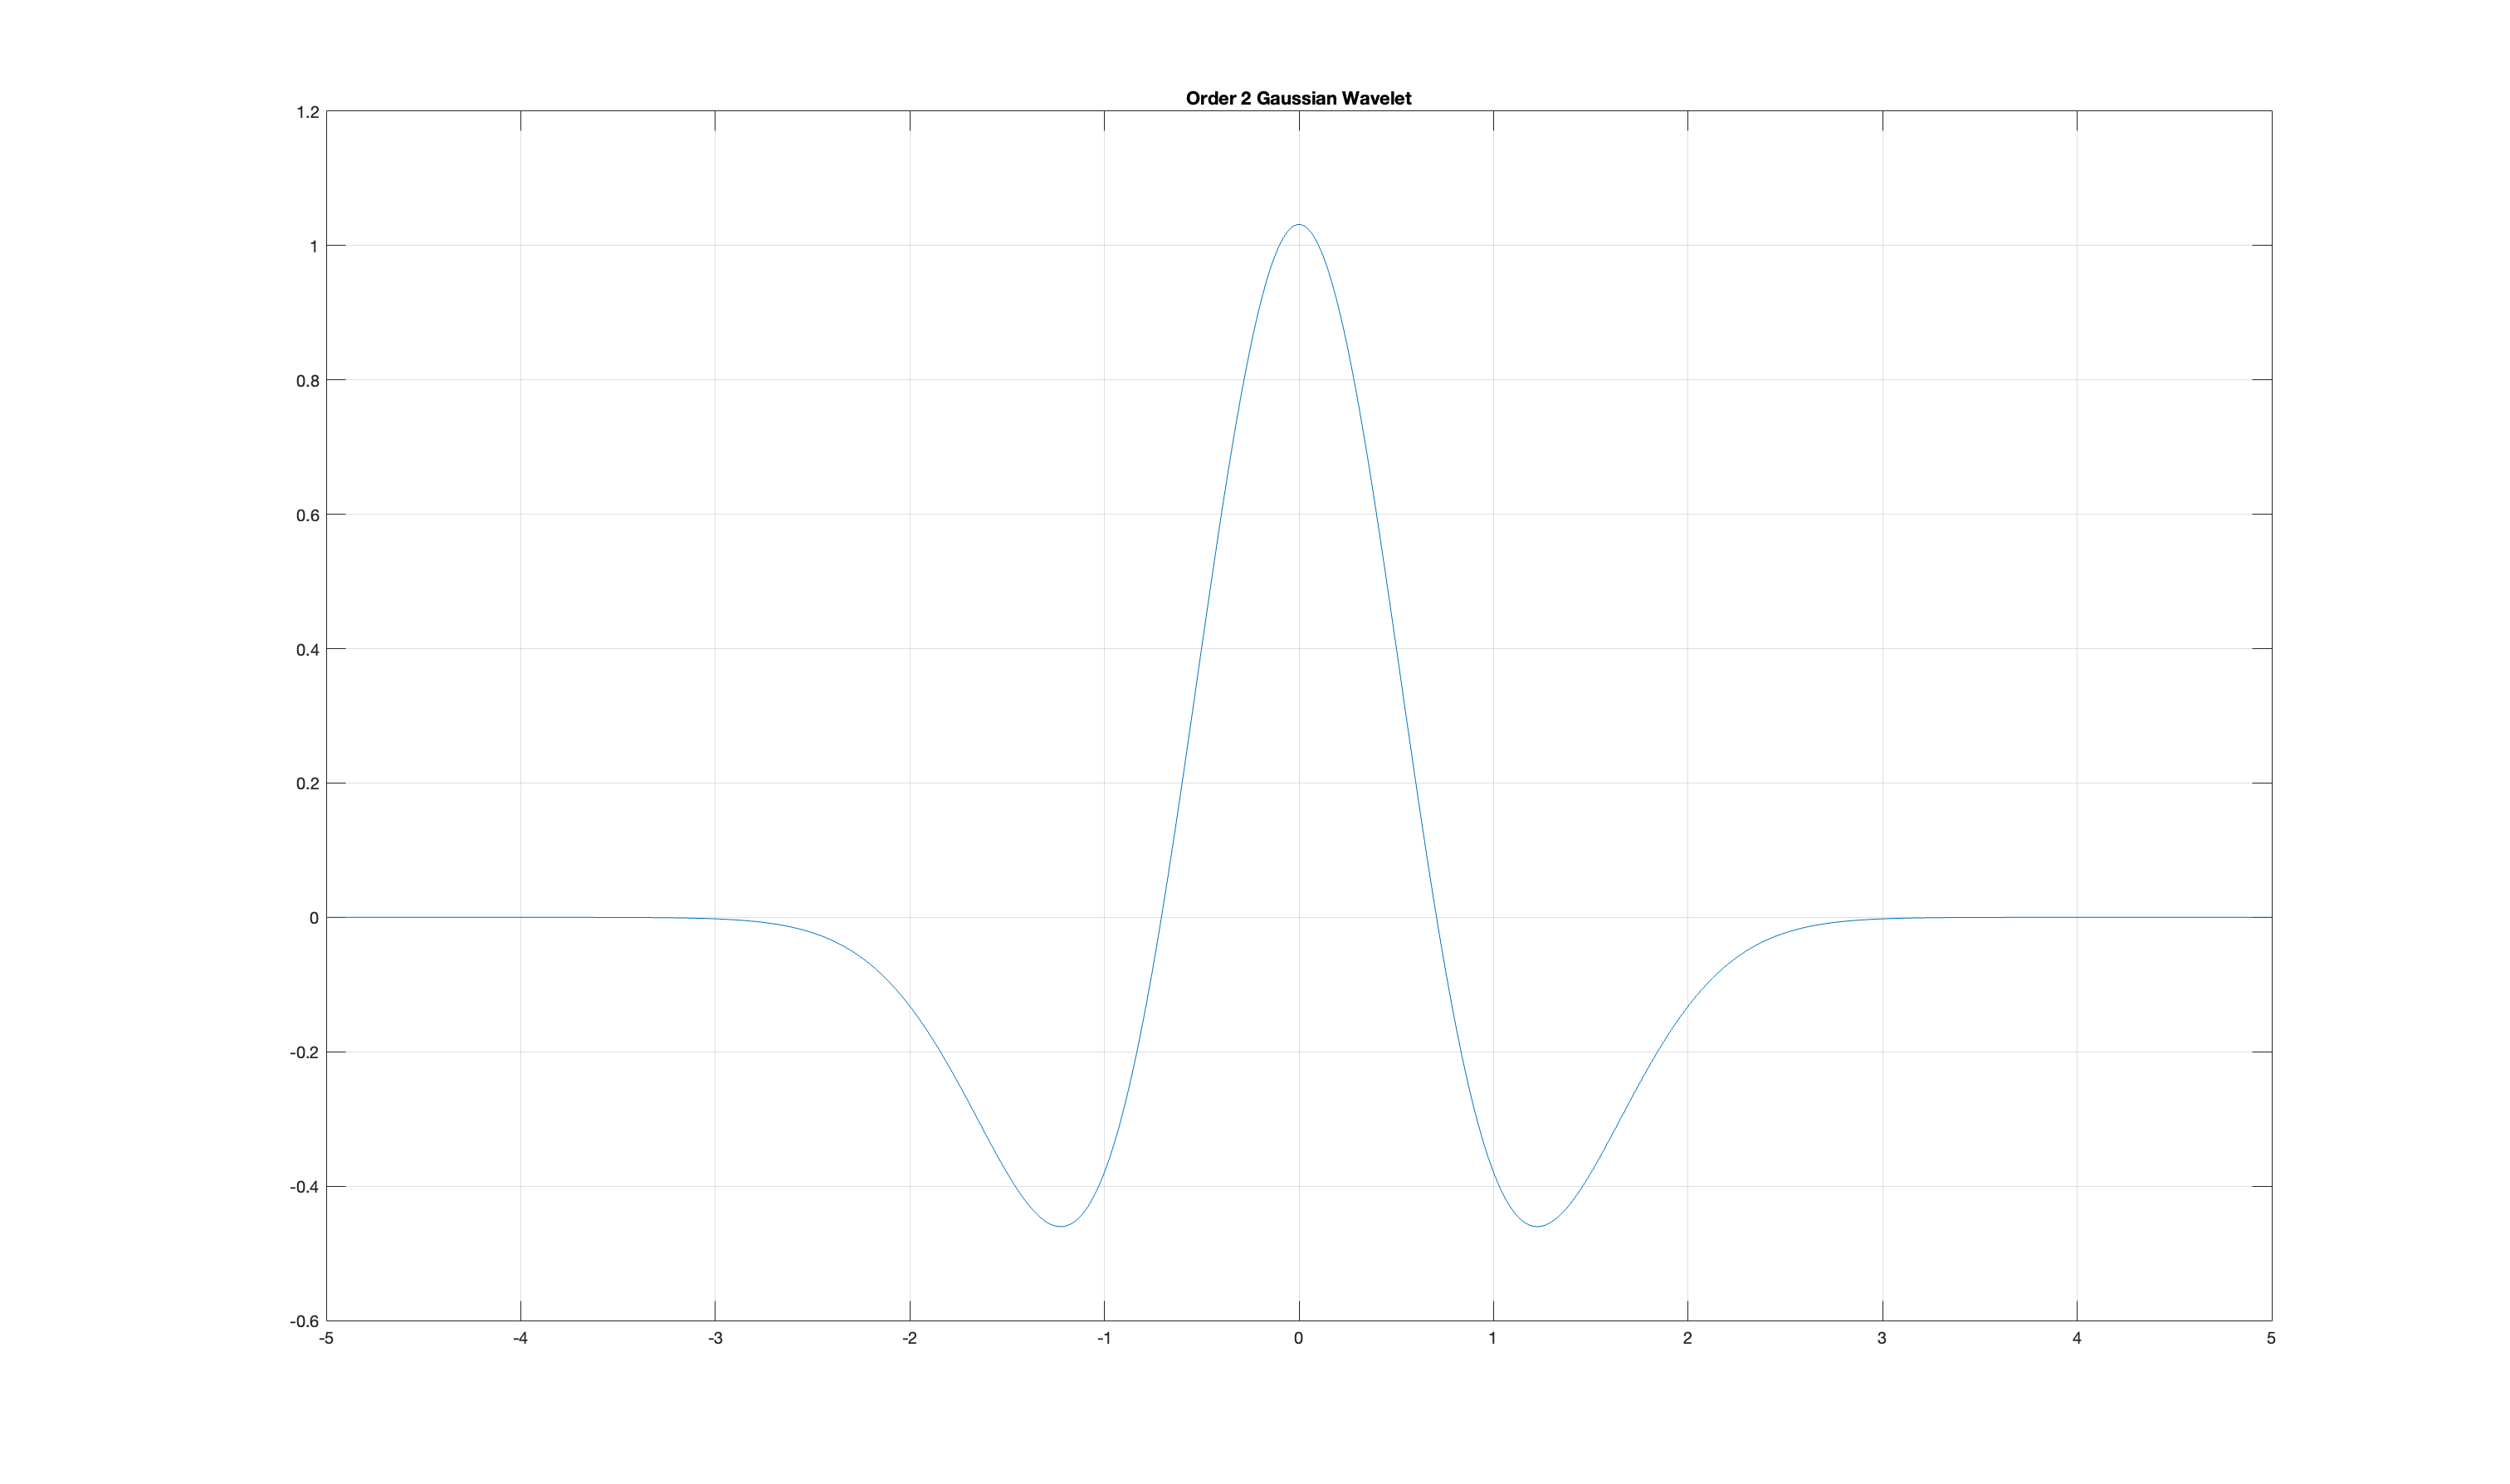
\includegraphics[width=\linewidth]{order2gaussian.png}
		  \caption{Ricker wavelet - Gaussian \\wavelet of order 2}
		  \label{Ricker}
		\end{subfigure}

		\caption{Examples of wavelets}
		\label{fig:test}
	\end{figure}
	
	The major difference between DWT and CWT is how the scale parameter is discretized. DWT discretizes scale parameters to integer power of 2 while CWT is more refined since 
	the scale parameter is often raised to different fractional powers.
	\begin{align*} &\text{DWT}\ [\mathrm{n},\mathrm{a}^{\mathrm{j}}]=\sum_{\mathrm{m}=0}^{\mathrm{N}-1}\mathrm{x}[\mathrm{m}].{\psi_{\mathrm{j}}}^{*}[\mathrm{m}-\mathrm{n}],\\ &\psi_{\mathrm{j}}[\mathrm{n}]=\frac{1}{\sqrt{\mathrm{a}^{\mathrm{f}}}}\psi\left(\frac{\mathrm{n}}{\mathrm{a}^{\mathrm{f}}}\right) \tag{2} \end{align*}
	where $n$ is delay parameter, $N$ is the length of signal, $\psi$ is the discretized mother wavelet\footfullcite{wavelet_denoise}. 

	DWT is often preferred in the context of real-time audio processing since computation is done on discrete wavelets which requires less computational resources.
	
	\item Spectral reduction\\
	Spectral noise gating learns from a noise profile and removes slow-changing tonal noise or hiss from the signal. In 
	fact, this method is used by Audacity in its noise reduction algorithm\footfullcite{audacity}. 
	Suppose noise is additive, and we can represent our noisy audio 
	\[y(n) = x(n) + d(n), \textit{for } 0 \leq n \leq N-1 \label{sreduction} \]
	where $x(n)$ is our original signal (the signal we wish to recover), $d(n)$ is the noise, $n$ is the discrete time index,
	$N$ is the number of samples. 
	Assuming $d(n)$ and $x(n)$ have no correlation, and we perform a short-time fourier transform on equation \ref{sreduction}:
	\[Y(\omega,k)= X(\omega,k) + D(\omega,k)\]
	where $k$ is the frame number, which can be dropped if we assume the signal is segmented. Each segment will be of
	length $N$. We then have the desired signal in frequency domain:
	\[X(\omega) = Y(\omega) - N(\omega)\]
	Since the statistics of the noise is unknown, we try to find an estimate of noise spectrum by calculating the time-averaged
	noise spectrum using parts of the recording that only contain ambient noise\footfullcite{reductionmanual}. 
	\[\hat{N}(\omega) = \textbf{E}[|N(\omega)|] = (1/N)\sum_{i=0}^{N-1}|N_i(\omega)|\]
	We then get the estimated signal spectrum
	\[\hat{X}(\omega) = Y(\omega) - \hat{N}(\omega)\]
	We then set a gain control for each frequency band so if the sound exceeded the threshold, the gain is set to 0 dB or a user-defined
	constant.
\end{enumerate}
%-----------------------------------
%	SUBSECTION 2
%-----------------------------------
\subsection{Choice of model and implementation}
After trying to implement all 3 methods, a major difficulty encountered is that it is hard to set the parameters to 
implement for LPF and wavelet transform.
For example, since $f_c$ depends on the pitch range of the user and the melody he/ she
is inputting, finding an adequate $f_c$ that separates desired frequencies from undesired ones is hard.
As for wavelet transform, finding an adequate mother wavelet is a difficult task.\\
Although wavelet transform works better for real-life non-stationary signals compared to conventional frequency-based filters, if we
do not feed a suitable mother wavelet, the performance is unsatisfactory, the model cannot distinguish between desired and undesired 
signals and will decrease $P_{signal}$ at the same time, which is unfavourable when it comes to improving the SNR.\\
According to \cite{complexwt}, there are 2 major concerns with using wavelet transform. 
Firstly, it is sensitive to shifting in time, even a minor shift will cause unpredictable change in transform coefficients which will 
then cause variations in the output signal. Secondly, wavelet transform suffers from poor directionality easily. For example, 
a 2-D DWT can only reveal 3 spatial-domain feature orientations, which limits the optimal representation of the signal. 

Therefore, we decided to use spectral reduction as our noise filter algorithm since it is the most effective in removing the ambient noise 
and wideband noise. Note that this method heavily relies on the assumption that the noise spectrum magnitude is staying locally 
stationary. If this assumption is not satisfied, this method will result in poor performance of either not being able to filter a majority of 
the broadband noise or removing the features of the signal.
The implementation of spectral noise gating can be summarised according to \cite{spectralflowchart} as shown in \autoref{spectralflowchart}
\begin{figure}
	\centering
	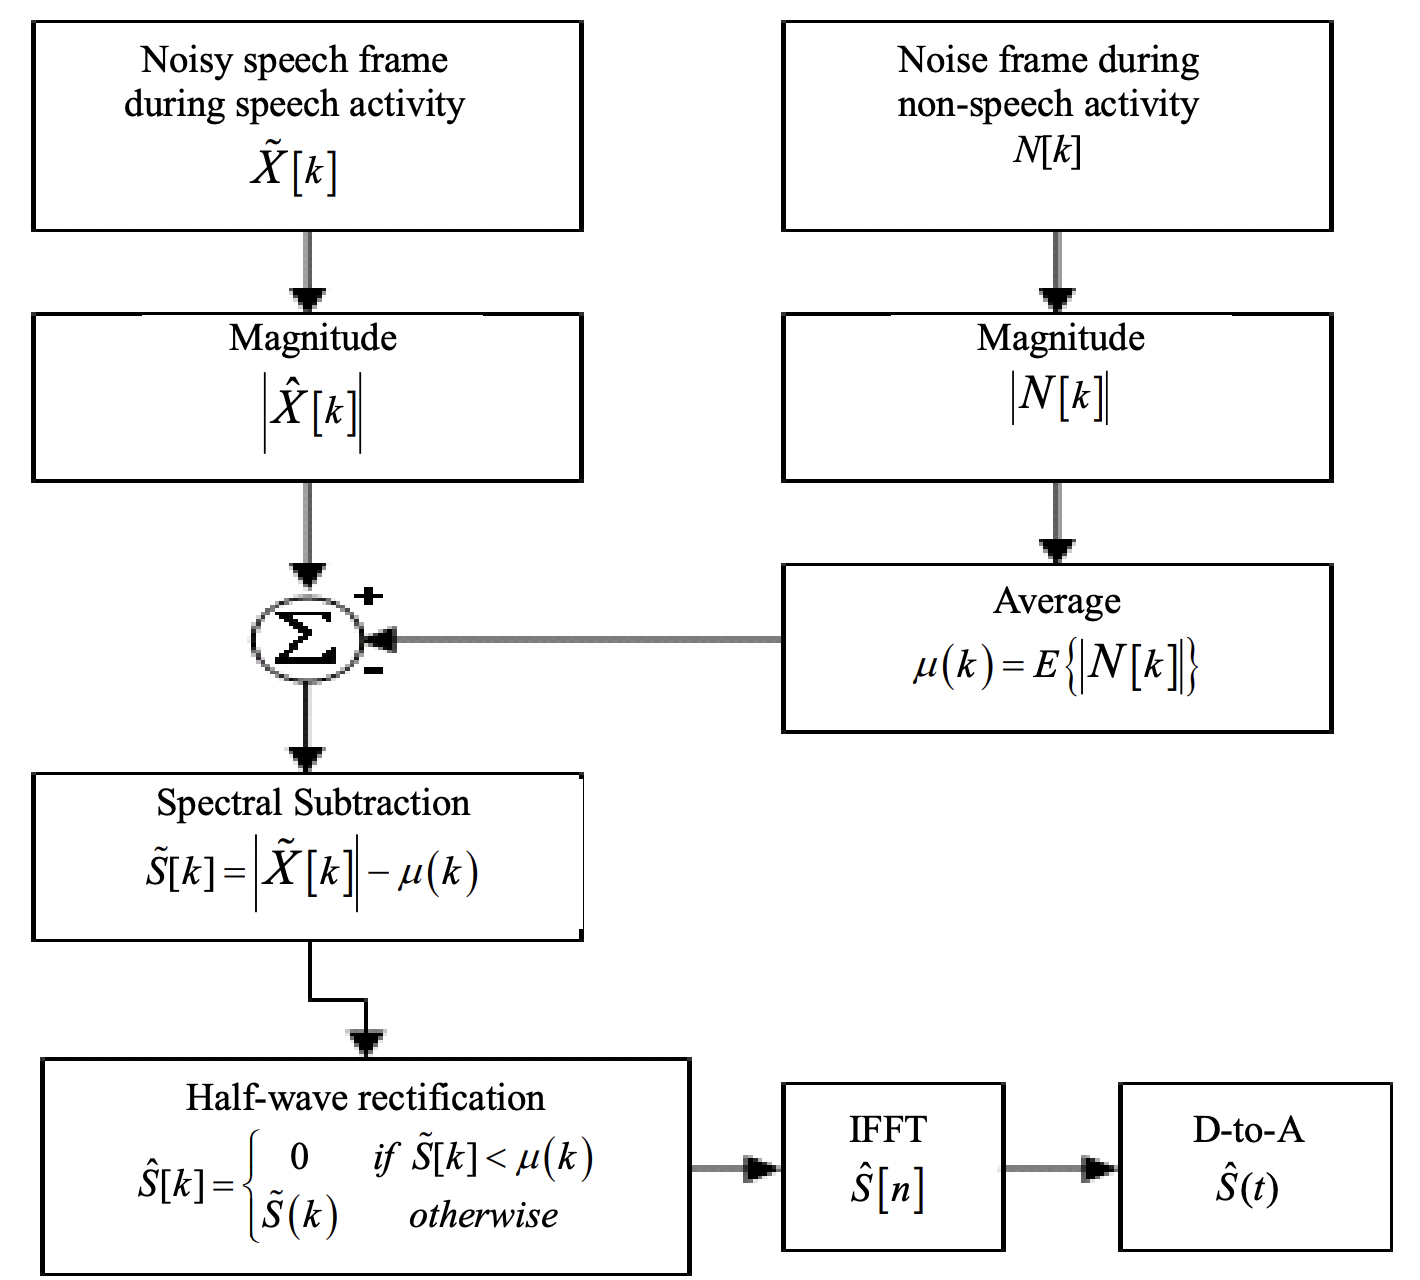
\includegraphics[scale=0.35]{spectralprocess.png}
	\caption{Spectral noise gating flowchart}
	\label{spectralflowchart}
\end{figure}
The noise spectrum $N(\omega)$ and its statistical measures are obtained by asking users to record at least 3 seconds of silence 
before they sing into the app.
Note that half-wave rectification is necessary after noise removal process of subtracting the average magnitude of noise spectrum.
This is to target frequencies that have a higher average magnitude of noise spectrum $\textbf{E}[|N(\omega)|]$ compared to that of 
the noisy speech spectrum $|\hat{X}(\omega)|$. For those frequencies, we would replace the negative values with 0 with a half-wave 
rectification.

%-----------------------------------
%	SUBSECTION 3
%-----------------------------------
\subsection{Improvements}
A drawback with spectral reduction is that it does not handle extreme responses nicely. It does not reduce noises like
squeaks. Also, since a half-wave rectification is included in the implementation process, \cite{spectral_drawback} has 
pointed out that residual noise will be created during the process of spectral reduction. Half-wave rectification introduces
nonlinearity in the $\hat{X}(\omega)$ spectrum and results in frequencies changing abruptly between frames.

As mentioned above, spectral reduction is built on the assumption that the noise is a stationary or slowly-varying. Yet in reality,
there may be sudden squeaky noise in the background which is not recorded in the noise profile. In this case, spectral reduction 
cannot remove the squeak. To improve the situation, we will introduce a low-pass filter to filter out high-frequency noise. The reason
for choosing LPF over a band pass filter is that spectral reduction is effective in targeting the reduction of ambient noise, which is
 usually low frequency. Thus as to avoid removing low-frequency desirable features, a low-pass filter will suffice.

To determine $f_c$ for the LPF, it would be plausible to refer to biological features of the users, i.e. their age and gender.
For males, the pitch level generally reduces from infancy to middle age, while a reversal of trend occurs after middle age. 
On the other hand, as pointed out by \cite{womenprange}, "Females in their 30s and 40s showed obviously lower frequencies than those in their
20s. Across all age groups, including the 80s, fundamental frequencies tended to decrease markedly in association with aging”

\begin{table}
	\begin{minipage}{0.45\linewidth}
		\label{table:praat}
		\centering
		\scalebox{0.9}{
		\begin{tabular}{lrr}		& Male   & Female  \\
			Pitch range (Hz)            & 60-180 & 160-300 \\
			Praat pitch range (Hz) 		& 50-300 & 100-600
		\end{tabular}}
		\caption{Praat pitch range}
		\end{minipage}\hfill
	\begin{minipage}{0.65\linewidth}
		\centering
		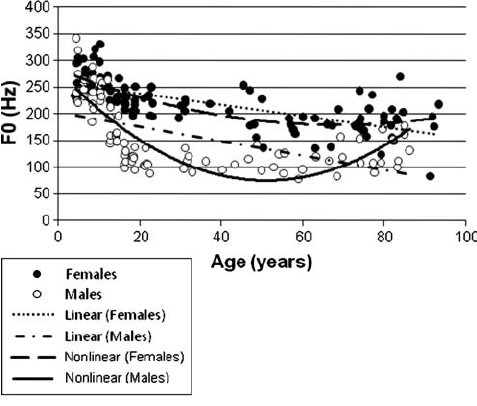
\includegraphics[scale=0.4]{f0vage.jpeg}
		\label{f0vage_chart}
		\captionof{figure}{Scatter plot of\\fundamental frequency by age}
	\end{minipage}
\end{table}

After referring to the measurements taken from 192 participants\footfullcite{f0age} and the pitch range
set by Praat\footfullcite{praat} (a software for speech analysis), a simple modelling of $f_c$ according to age and gender
is as below:
\[f_{c,male}(n) = 0.07n^2 - 7.5n + 280, \text{for } 4 \leq n\leq 93 \label{male} \] 
\[f_{c,female}(n) = 0.02n^2 - 3n + 287, \text{for } 4 \leq n \leq 93 \label{female} \] 
where $n$ is the age of the user
In deciding which filter to implement, there are 3 filters in consideration:
\begin{enumerate}[label=(\alph*)]
	\item Type 1 Chebyshev filter
	\[G_{n}(\omega) = |H_{n}(j\omega)| = {\frac{1}{\sqrt{1+\varepsilon^{2} T_{n}^{2}(\frac{\omega}{\omega_{0}})}}}\]
	where $\varepsilon$  is the ripple factor, $\omega _{0}$ is the cut-off frequency
	and $T_{n}$ is a Chebyshev polynomial of the $n$th order.
	\item Butterworth filter
	\[G_{n}(\omega) = |H_{n}(j\omega)| = {\frac{1}{\sqrt{1+(\frac{\omega}{\omega_{0}})^{2n}}}}\]
	where $\omega _{0}$ is the cut-off frequency and $n$ is the order of filter.
	\item Bessel filter
	\[G_{n}(\omega) = |H_{n}(j\omega)| ={\frac {\theta _{n}(0)}{\theta _{n}(\frac{j\omega}{\omega _{0}})}}\]
	where $\theta _{n}(j\omega)$ is a reverse Bessel polynomial and $\omega _{0}$ is the cut-off frequnecy
\end{enumerate}

Chebyshev filter has a steeper roll-off compared to Butterworth and Bessel filter, but it also brings passband and stopband ripples, 
unlike Butterworth and Bessel filter which have a flat passband and stopband as they roll off towards zero. Moreover, Butterworth 
and Bessel filters have a better step response. Meanwhile, Bessel filters perform the best in step response since the overshoot is
minimal. Also, an important characteristics Bessel filter has is that it introduces a linear-phase and constant delay for $f<f_c$. This
feature allows us to preserve the waveshape since all frequencies are delayed by the same amount.
Thus, Bessel filter is preferred in this context.

\begin{figure}[h]
	\centering
	\begin{subfigure}{.32\textwidth}
	  	\centering
	  	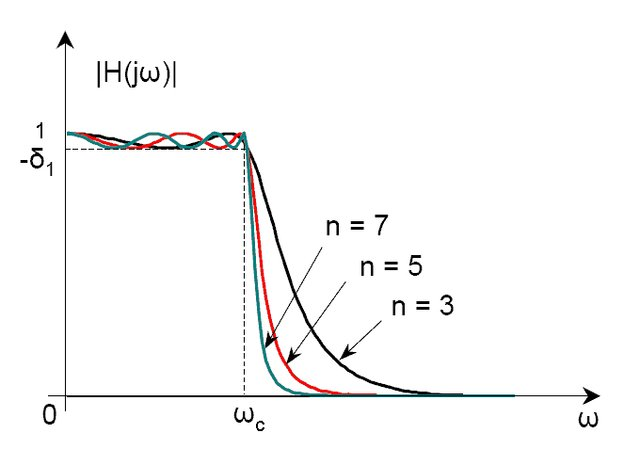
\includegraphics[width=1\linewidth]{chebyshev.jpeg}
	  	\caption{Type 1 Chebyshev filter \\frequency response}
	  	\label{fig:sub1}
	\end{subfigure}
	\begin{subfigure}{.32\textwidth}
	  	\centering
	  	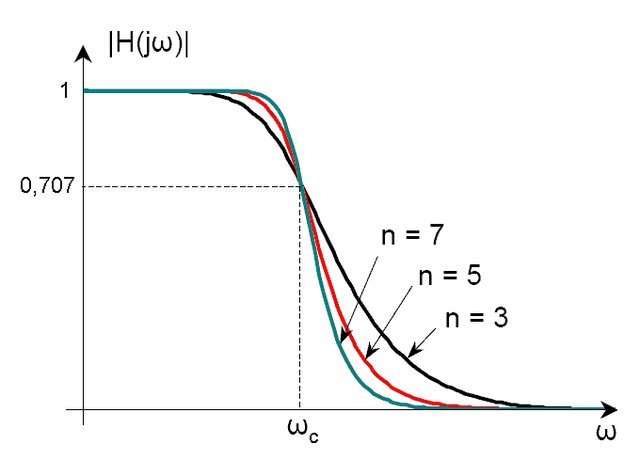
\includegraphics[width=1\linewidth]{butterworth.jpeg}
	  	\caption{Butterworth filter frequency response}
	  	\label{fig:sub2}
	\end{subfigure}
	\begin{subfigure}{.32\textwidth}
		\centering
		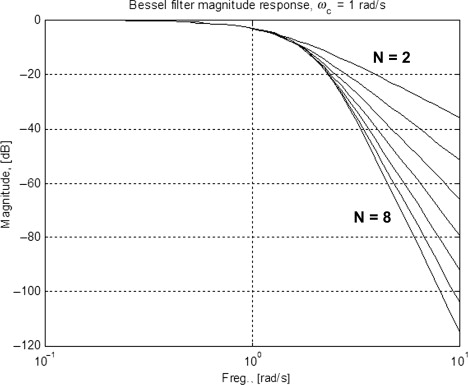
\includegraphics[width=1\linewidth]{bessel.jpg}
		\caption{Bessel filter frequency\\response %\footfullcite{bessel}%}
		\label{fig:sub3}
	\end{subfigure}
\end{figure}

%----------------------------------------------------------------------------------------
%	SECTION 2
%----------------------------------------------------------------------------------------
\section{Pitch Detection Algorithm (PDA)}
\label{sec:PDA}
After removing noise, we pass the processed signal to a PDA to estimate the fundamental frequency ($f_0$) of
the signal.

%-----------------------------------
%	SUBSECTION 1
%-----------------------------------
\subsection{Possible Models}
There are 4 approaches to detect $f_0$, which can be classified into time domain and frequency domain.

\begin{enumerate}
	\item Zero crossings (time domain)\\
	This is the most intuitive method to detecting pitch although it suffers from low accuracy.
	Assuming the input is monophonic, the fundamental frequency is estimated as:
	\[f_0 = \frac{P_{zcr}f_s}{2N}\]
	where $P_{zcr}$ is the number of zero-crossing points, $f_s$ is the sampling rate,
	$N$ is the number of samples.
	\begin{figure}[h]
		\centering
		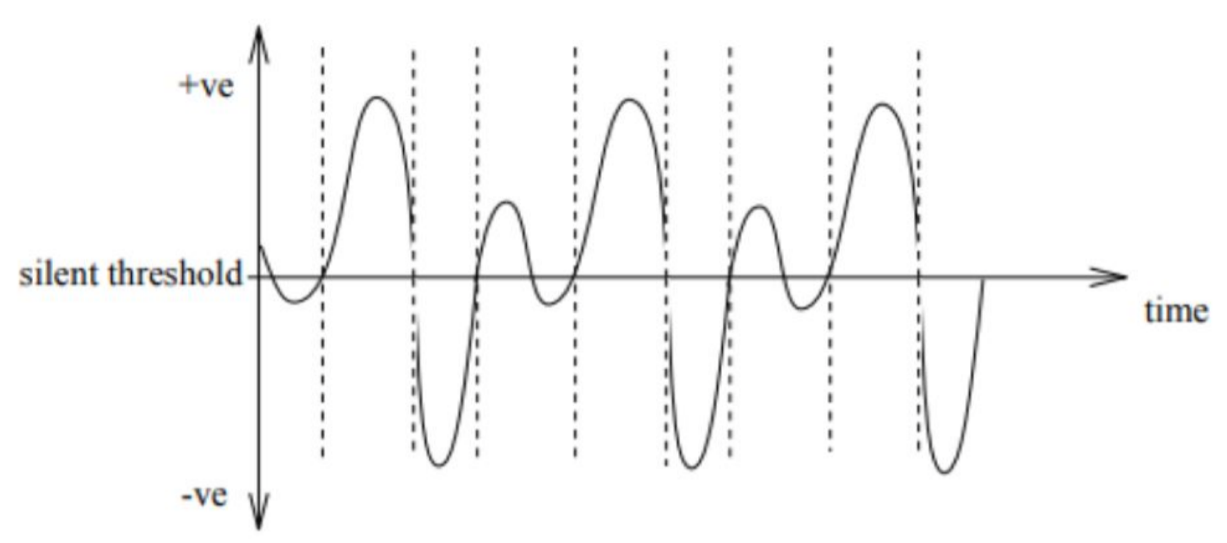
\includegraphics[width=0.5\textwidth]{zcr.png}
		\caption{An example signal with zero-crossings marked in dotted lines \footfullcite{zcr}}
	\end{figure}

	\item Harmonic Product Spectrum (HPS) (frequency domain)\\
	As aforementioned, human voice is not of pure tone, a musical note sung will consist of a series of peaks in its frequency spectrum,
	which the peaks corresponds to $f_0$ with other peaks indicating the harmonic components of integer multiples of $f_0$. 
	Exploiting this fact, HPS algorithm creates multiple downsampled signal spectrums and compares them wiht the original spectrum as shown in figure 
	\ref{HPS}. The strongest harmonic peak will line up no matter how many times we compress the spectrum.
	
	\begin{figure}[h]
		\centering
		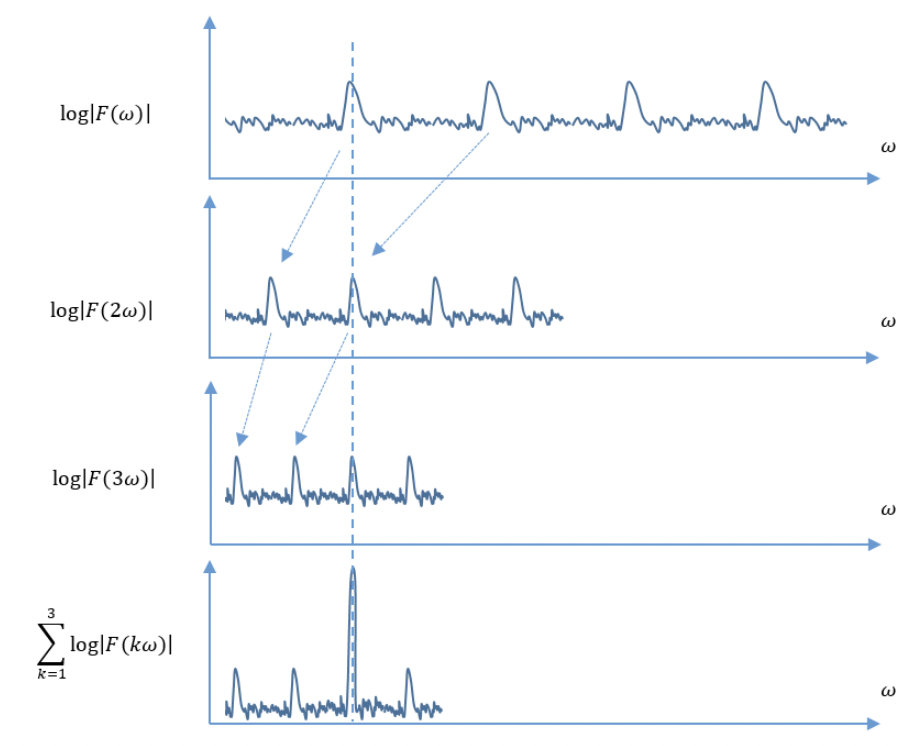
\includegraphics[width=0.5\textwidth]{HPS.png}
		\caption{Harmonically compressed log spectra \footfullcite{HPS}}
		\label{HPS}
	\end{figure}
	
	Firstly, we convolve the signal with a Hanning window to segment the input:
	\[w(n) = \frac{1+cos(2\pi n/N-1)}{2}, \text{ for } 0 \leq n \leq N-1\] where $N$ is the number of samples.\\
	We then convert it from time-domain to frequency-domain by computing the short-time Fourier Transform:
	\[STFT \{x[n]\}(k,\omega) = X(k,\omega )= \sum _{n=-\infty }^{\infty }x[n]w[n-k]e^{-j\omega n}\]
	Lastly we compute the product of spectrum at harmonics of various frequencies and $f_0$ is estimated by:
	\[f_0 = argmax\prod_{k=1}^{n}|X(kf)|\] 

	\item YIN algorithm/ autocorrelation (time domain)\\
	As outlined by \cite{yin}, YIN algorithm is based on a slightly altered autocorrelation method:
	\[r_t(\tau)=\sum_{j=t+1}^{t+W-\tau}x_j x_{j+\tau}\]
	where $r_t(\tau)$ is the autocorrelation function (ACF) of lag $\tau$ calculated at time index $t$, $W$ is the integration
	window size. Note that as $\tau$ increases, $W$ decreases and the envelope of the function decreases, as shown in figure 
	\ref{taped}.

	\begin{figure}
		\centering
		\begin{subfigure}{.3\textwidth}
		  \centering
		  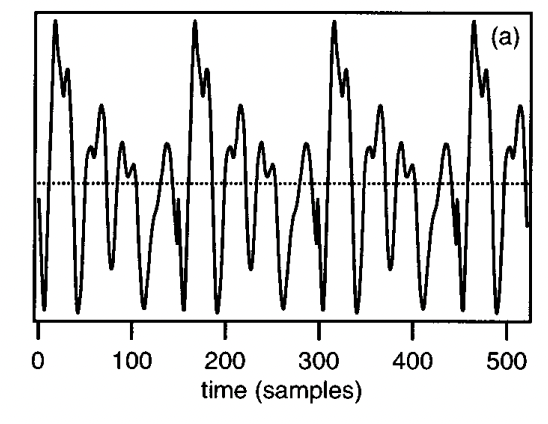
\includegraphics[width=1\linewidth]{signalwaveform.png}
		  \caption{Signal waveform}
		  \label{signal}
		\end{subfigure}%
		\begin{subfigure}{.3\textwidth}
			\centering
			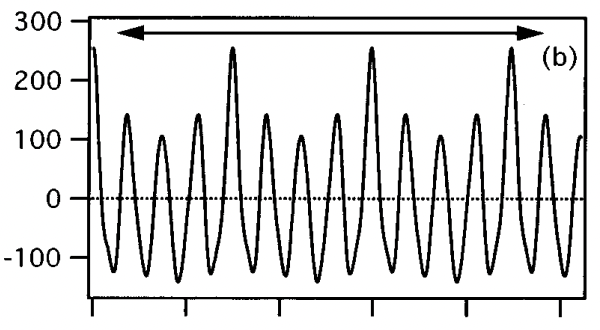
\includegraphics[width=1\linewidth]{acf.png}
			\caption{$r_t(\tau)$ calculated from \\figure \ref{signal} using normal ACF}
			\label{acf}
		  \end{subfigure}%
		\begin{subfigure}{.3\textwidth}
		  \centering
		  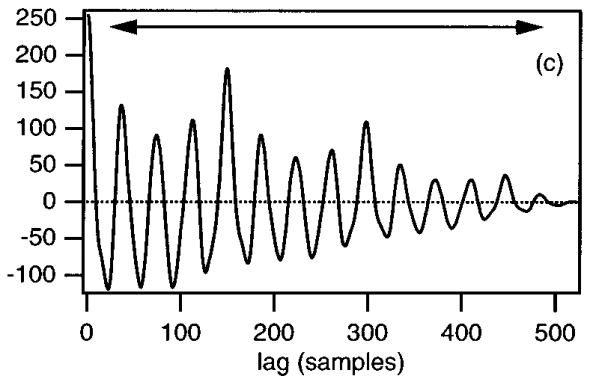
\includegraphics[width=1\linewidth]{taperedacf.png}
		  \caption{$r_t(\tau)$ calculated with equation \ref{signal}}
		  \label{taped}
		\end{subfigure}%
		\label{YIN}
	\end{figure}
	
	We then select the highest peak by exhaustive search within an user-defined range of lags, the corresponding time lag will be
	the inverse of our estimated $f_0$.

	To improve the error rates and target periodicity, de Cheveigné \& Kawahara introduced a cumulative mean normalized difference function (CMNDF)
	to replace ACF. 
	\begin{equation}
		CMNDF(\tau) = \begin{cases}
			 1             & \text{if $\tau = 0$} \\ 
    		\frac{DF(\tau)}{(1/\tau)\sum_{j=1}{\tau} DF(j)} & \text{otherwise.}
		\end{cases}
	\end{equation}
	
	We then find $\tau$ that minimises $CMNDF(\tau)$ and the corresponding $f_0$.

	\item CREPE (Convolutional Representation for Pitch Estimation) (Machine learning method)\\
	CREPE is a data-driven algorithm developed by Kim et al. that operates directly on the time-domain.
	It consists of a deep convolutional neural network (CNN) trained by synthesized audio from the RWC Music Database \footfullcite{rwcdb}
	and MedleyDB \footfullcite{medleydb}. 

	CNN is often seen in image-processing application and is a network that makes use of convolution instead of the typical matrix multiplication..
	It consists of an input layer, hidden layers and an output layer. Hidden layers includes convolution layers, pooling layers and fully connected layers.
	
	As shown in figure \ref{CREPE}, there are 6 hidden layers and each layer is followed by a dropout layer with dropout probability of 0.25. 

	Convolution layer are the building blocks of CNN since it performs feature extraction through convolution and activation function like $ReLU$.
	There are 2 hyperparameters that define a convolution operation, which are the kernel size and number of kernels. Kernels in the convolutional layer context are convolutional
	filters, so that kernel size refers to the size of filter mask and number of kernels relates to the number of output features desired. Figure \ref{CREPE} shows the hyperparameters
	used in CREPE.

	Max pooling is often used in the operation of pooling layer and is the operation used in CREPE. It outputs the maximum value in a patch extracted from the
	input tensor and discards the non-maximum values. 
	One advantage of using max pooling is that it suppresses noise better than other dimensionality reduction methods like average pooling.

	A fully connected layer maps all extracted features in one layer to every activation unit of the next layer. In the context of CNN, it is often seen in the
	last few layers to compile the features for final output.

	\begin{figure}
		\centering
		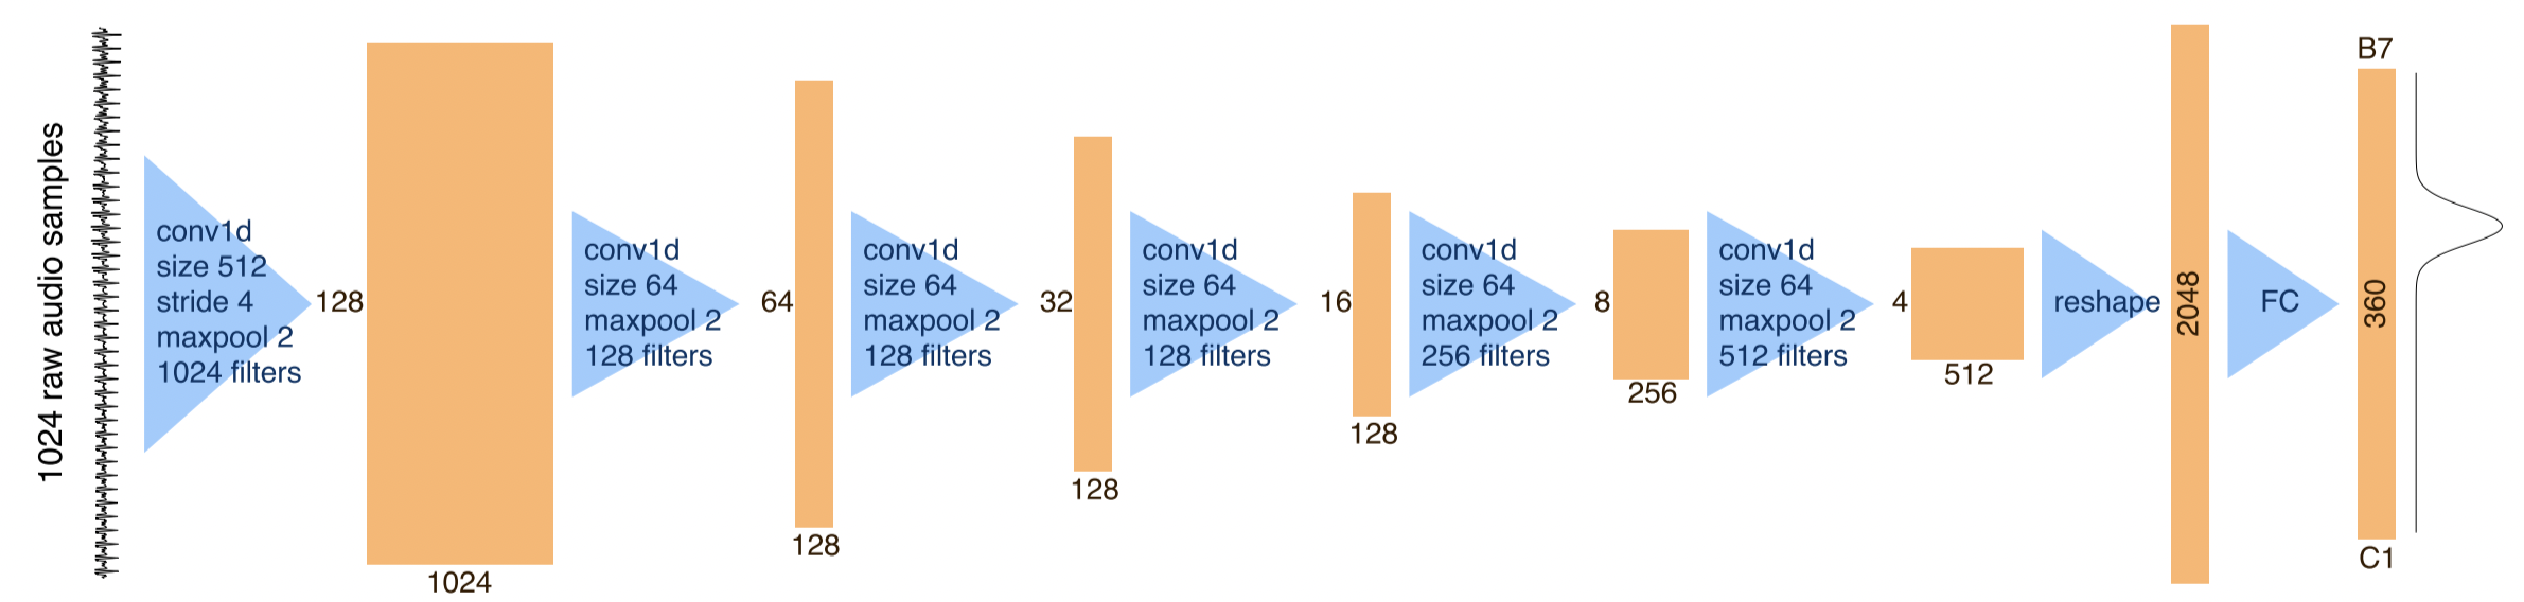
\includegraphics[scale=1.5]{CREPE.png}
		\caption{The architecture of the CREPE algorithm\footfullcite{CREPE}}
		\label{CREPE}
	\end{figure}
	%The model is trained with 5-fold cross-validation and a 60/20/20 train, validation and test split.

\end{enumerate}

%-----------------------------------
%	SUBSECTION 2
%-----------------------------------
\subsection{Comparison between models and implementation}
The zero crossings method will not be considered though it has the cheapest computational cost. One limitation is that
the threshold is fixed at 0, making it susceptible to noise and the vocal timbre of the user. Moreover, the method heavily relies on
the assumption that the input audio is of pure tone but unlike a tuning fork, human voice is not a pure tone. It is 
composed of a fundamental frequency and upper harmonics\footfullcite{humanmono}.  This characteristic makes this method extremely
unreliable.

Like the zero-crossings method, HPS is intuitive and has little computational cost. But since it builds on the characteristics 
that the signal contains amplitudes at harmonics, if the input signal does not have sufficient magnitudes at other harmonics, the 
performance of HPS will suffer. Moreover, the resolution of the method depends on the length of short-time Fourier Transform, which
determines the number of discrete frequencies that we can consider. But if we want a higher resolution and less graininess in our 
pitch output, more time is needed in performing the transform.

YIN has a more satisfactory performance but when the pitch varies rapidly (for example if the user has a breathy timbre), it cannot 
estimate the pitch correctly as the algorithm uses a constant threshold. On the other hand, Kim et al. mentioned CREPE has a higher 
tolerance for inputs with different timbres since CREPE is trained with MedleyDB which contains recordings heterogeneous timbres. Figure 
\ref{CREPEperf} concludes the Raw Pitch Accuracy and Raw Chroma Accuracy for CREPE and other 2 PDA by Kim et al. and we will choose CREPE 
to implement in our model.

\begin{figure}[h]
	\centering
	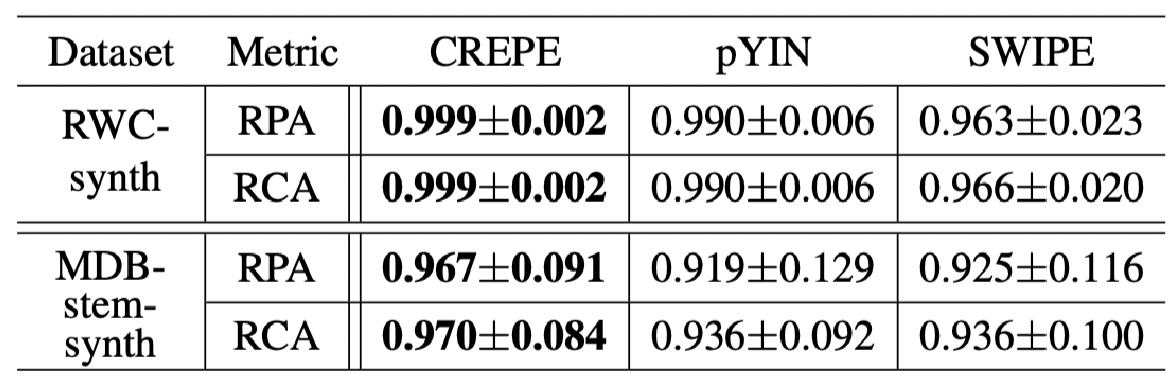
\includegraphics[scale=1.5]{CREPEperf.png}
	\caption{Raw Pitch Accuracy and Raw Chroma Accuracy with the standard deviations for the 3 PDA tested by Kim et al. \footfullcite{CREPE}}
	\label{CREPEperf}
\end{figure}

The CREPE code uploaded by Kim et al. takes in the samples $y$, sampling rate $sr$ and a boolean parameter (True/ False) for viterbi, which is a smoothing algorithm. 
It calculates pitch every 10 ms and outputs the timestamp, estimated frequency $\hat{f_0}$, confidence $c$ and an activation matrix for visualization of outputs. 

The sampling rate of training data used by CREPE is at 16 kHz thus our input audio will need to be resampled to 16 kHz if the original $sr \neq 16 kHz$. If the user is using the iPhone 
built-in microphone to record, we need to set the preferred sampling rate to 16 kHz \footfullcite{iphoneaud} when coding for our iOS app.

One thing to note is that the algorithm centers the first frame at $t=0$ instead of starting the first frame at $t=0$ to avoid misalignment.

Continuing from the noise filtered signal, we use \emph{[y, sr]= scipy.io.wavfile.read(filename, mmap=False)} function to read the input and feed $[y, sr]$ 
into \emph{crepe.predict(y, sr, viterbi=True)}.
The output will be of the form [timestamp, $\hat{f_0}$, $c$, activation matrix].

We then manipulate the $\hat{f_0}$ array such that
\[\hat{f_0}= 
\begin{cases}
    \hat{f_0},		& \text{if } c\geq 0.5\\
    0,              & \text{otherwise}
\end{cases}
\label{creperesult}
\]
and omit frequencies that lasted less than 10 timeframes (0.1s).
%-----------------------------------
%	SUBSECTION 3
%-----------------------------------
\subsection{Improvements}

On top of the convolutional neural network model, we can integrate Bayesian statistics to improve the model.

Bayes' rule states: 
\[P(A\mid B)=\frac {P(B\mid A)P(A)}{P(B)}\]
where $P(A\mid B)$ is the posterior probability or the updated probability with the consideration of evidence.\\
$P(B\mid A)$ is the likelihood, which is the probability of observing the evidence given the event has happened.\\
$P(A)$ is the prior probability, which is the probability before taking into consideration the evidence.\\
$P(B)$ is known as the marginal probability, which is the probability of an event irrespective of outcomes of any evidence. \\

With enough audio samples sung by the user, we can collect the range of pitches that he/she manages to sing. Then we can model 
the probability distribution $P(x)$ to update the likelihood of observing a certain pitch given the previous audio samples.

The prior $P(A)$ can be obtained from the demographic characteristics collected, i.e. age and gender, with the afore modelled equation
\ref{male} and equation \ref{female}.

%----------------------------------------------------------------------------------------
%	SECTION 3
%----------------------------------------------------------------------------------------
\section{Key Detection Algorithm (KDA)}
\label{sec:KDA}
Other than detection the pitch/ note of the input audio, it is also necessary to estimate the key of the music so as to aid the identification
of chords with the machine learning model in the later step.

From a music theory point of view, the most intuitive method to identify the key of a piece is to look at the key signature which contains the number of sharps/ flats
in a piece, and the number defines which key the piece is in. But since our app targets amateurs, we will not expect them to be able to know what key will they be singing
in.

Krumhansl-Schmuckler algorithm (template-based) \footfullcite{template} is an experimentally measured tonal hierarchy is introduced by \cite{templatedata}, in which it contains 
24 tonal profiles for major and minor keys in total.
Each of the profiles contains 12 values which correponds to 12 notes in an octave. The values were obtained from the experiment where they asked the listeners to judge how well
a note fits in a key on a scale from 1 to 7 (1 stands for very bad, 7 stands for very good). We then calculate the correlation of distribution with these 12 major and 12 minor
templates. The key with the highest correlation will be the estimated key.

Yet, one drawback is that the sense of key changes over time as affected by the evolution of music. While the method can still be utilised, the template will have to be
updated from time to time.

\subsection{Implementation}
Assuming we are using the template from Krumhansl and Kessler\footfullcite{templatedata} in our model and it is represented as 24 vectors $\vec{P_{i,k}} \in \mathbb{R}^{12 \times 1}$, 
where $i$ is the tone of the profile, $j$ indicates whether the profile is in major or minor.
We also define the pitch class distribution (our input) as a vector $D \in \mathbb{R}^{12,1}$, where the 12 entries are the frequencies of the 12 notes that appeared in the audio.
$\vec{D}$ can be obtained by looping over the $\hat{f_0}$ array obtained in \autoref{creperesult} and using the Python function \emph{collections.Counter([iterable-or-mapping])} to count the
number of occurrences. We then calculate the correlation between $\vec{P_{i,k}}$ and $\vec{D}$, which is essentially the dot product between the two.
\[ corr(\vec{P_{i,k}},\vec{D}) = \vec{P_{i,k}} \cdot \vec{D} \]
The estimated key ($i,j$) is found by looping over the 24 $\vec{P_{i,k}}$ vectors and finding the one that gives the maximum correlation. 

% Chapter Template
\tocdata{toc}{Terence Tan}

\chapter{Training Data \& Data Processor} % Main chapter title

\label{Chapter3} % Change X to a consecutive number; for referencing this chapter elsewhere, use \ref{ChapterX}

As illustrated in \textbf{REFERENCE Figure 1.1}, the data from the voice processor will be passed to a data processor to convert it into the appropriate input data format for the machine learning model. But before that, the model has to be trained first in order to be of any use. Hence, we shall look at the dataset used to train and test the model before discussing the data processor in Section \ref{data processor}.

The processing of the raw dataset into the training/testing dataset had been carried out; the code and resulting datasets can be found on \textbf{REFERENCE GITHUB}. The data processor itself has not been coded but would be easy to create by re-using the code used to process the raw dataset.
%----------------------------------------------------------------------------------------
%	SECTION 1
%----------------------------------------------------------------------------------------

\section{Dataset}
Papers that worked on similar chord generation problems \cite{MySong} \cite{BLSTM} \cite{MLForChords} obtained their dataset by collecting lead sheets from public and private sources and preprocessing them. Unfortunately, most of them did not publicly share their processeed dataset. We could collect and preprocess our own lead sheets, of which there are quite a few possible sources such as MuseScore and the Million Song Dataset \cite{Bertin-Mahieux2011}. However, \cite{BLSTM} do provide their preprocessed dataset in which the features of the lead sheets have already been extracted. Given that extracting the musical features ourselves would be time-consuming, and that we are building a Minimum Viable Product that would not require an extensive dataset, we decided to use that dataset.

There are 2252 songs in this dataset, 1802 of which had been categorised as the training set while the remaining 450 had been categorised as the test set. Each song is in major key and only have a single chord per bar. For each song, all the relevant features had been extracted and placed into a single \emph{CSV} file. These files can then be read and converted to DataFrame format using Python \emph{Pandas} as shown in Figure \ref{fig:CSV_DF}.

As can be seen in Figure \ref{fig:CSV_DF}, the rows each contain information about a single note. Each bar is taken to be a single measure. The columns each represent a different piece of information about that particular note. \emph{time} refers to the time signature, \emph{measure} refers to the measure to which that particular note belongs to, \emph{key\_fifths} indicates the number of sharps/flats (e.g. -1 for one flat and 1 for one sharp), \emph{chord\_root} is the root of the chord with \emph{chord\_type} indicating the type of chord, \emph{note\_root} identifies the particular single note of that row, \emph{note\_octave} is the octave of that note, and \emph{note\_duration} indicated the duration of the note (4.0 for a quarter note).

\begin{figure}
\centering
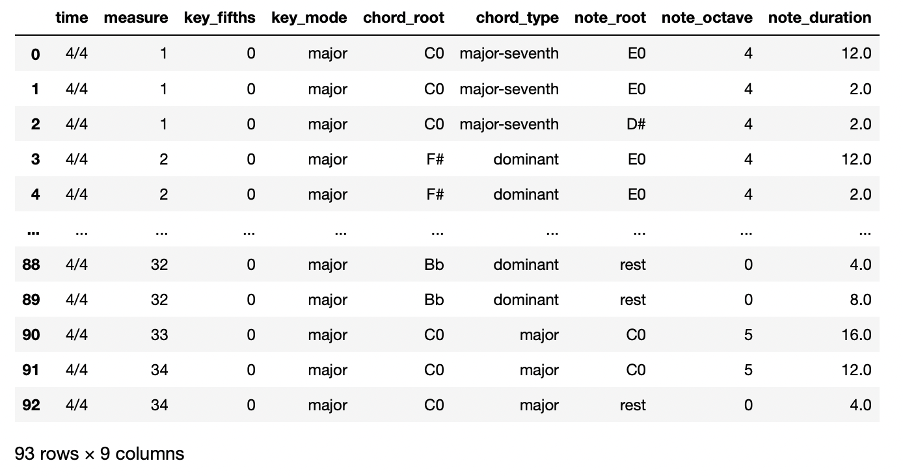
\includegraphics{Figures/CSV dataframe}
\decoRule
\caption{A song in DataFrame format after being read from CSV file}
\label{fig:CSV_DF}
\end{figure}

%-----------------------------------
%	SECTION 2
%-----------------------------------
\section{Preprocessing of dataset}
\label{preprocessing}

The dataset can be preprocessed to remove unnecessary information in order to make the dataset cleaner and ready for conversion into input formats that are compatible with our machine learning models. Steps 1-5 listed below are based on the preprocessing done in the other papers that worked on similar chord generation problems \cite{MySong} \cite{BLSTM} \cite{MLForChords}. We paid particular attention to the preprocessing steps of the paper \cite{BLSTM} from which we obtained our dataset.

\begin{enumerate}
  \item All songs are transposed to C major key. The key of a song determines the notes and the set of chords present in the song. Transposing all songs to a common key will normalise the different features of melodies and chords in different songs. The number of chord types present in the dataset will be reduced, which will decrease the number of chord types during the training process. Each song can be shifted to a different key without loss of the song's subjective character by shifting all the pitches equally \cite{MySong} \cite{MLForChords} \cite{BLSTM}.
  \item The time signatures are all normalised. Since different songs have different time signatures, each \emph{note\_duration} is multiplied by the reciprocal of the time signature \emph{time} to give a normalised note duration \cite{BLSTM}.
  \item Chord types are restricted to major and minor chords since having all chord types exist as independent classes will result in too few datapoints for each chord type \cite{BLSTM}. All other chord types are converted to their most similar major or minor chords by simplifying them to their core triads. This would result in loss of some emotive character, but would not sigficantly degrade the appropriateness of a chord for a particular melody segment \cite{MySong}. Note that more chord types can be easily added to our model in the future by adding more columns to the data input matrix in Section \ref{LSTM format for training} and by including more class types in the chord sequence in Section \ref{Transformer format for training}.
  \item Some measures in the dataset contain rest notes. These measures can be removed from the dataset \cite{MLForChords}.
  \item Octave information is not required and is removed from the dataset \cite{BLSTM}.
  \item There are also some irregular notes present in the dataset such as 'B-2' and 'A2' as shown in Figure \ref{fig:notefreq} using the \emph{value\_counts()} function. Further analysis shows that the numbers after the letters do not seem to represent octave or any other information; as can be seen in Figure \ref{fig:irregnote}, the indexed measures all have a \emph{note\_root} of 'B\-2' but do not all share a commonality in any of the other columns (excluding \emph{key\_mode} which would be 'major' for all measures since the dataset only contains songs in the major key). The paper from which this dataset was obtained also made no mention of these irregular notes. Given that they represent a very small portion of the dataset (41 measures as calculated from Figure \ref{fig:notefreq}), measures containing these irregular notes are removed.
\end{enumerate}

\begin{figure}
    \centering
    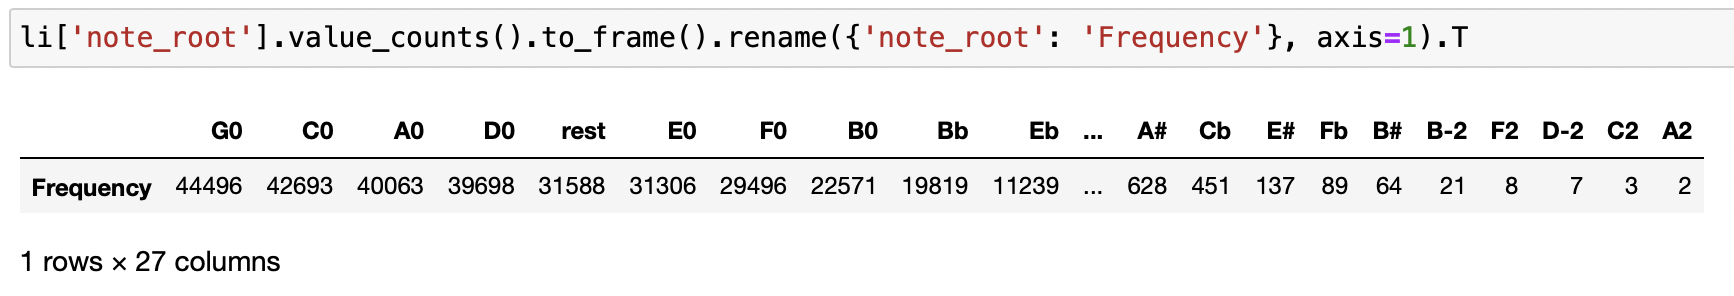
\includegraphics[scale=0.5]{Figures/note frequency}
    \decoRule
    \caption{Number of each \emph{note\_root} (frequency) that exists within the entire dataset.}
    \label{fig:notefreq}
    \end{figure}
    
    \begin{figure}
        \centering
        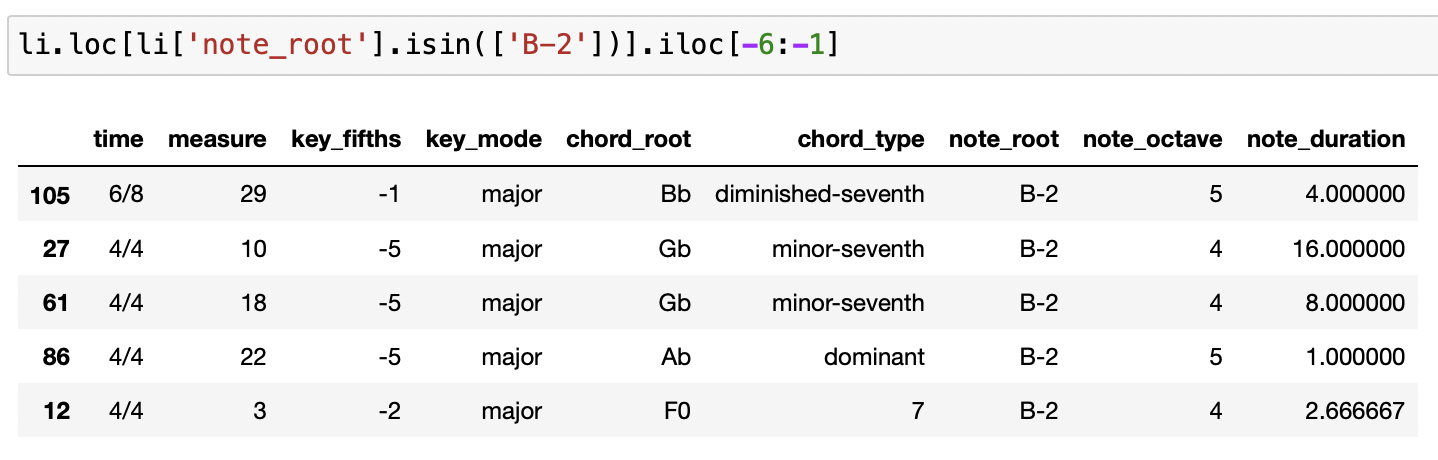
\includegraphics[scale=0.5]{Figures/irregular notes}
        \decoRule
        \caption{Indexed measures containing \emph{note\_root} of 'B\_2'.}
        \label{fig:irregnote}
        \end{figure}
        
%-----------------------------------
%	SUBSECTION 1
%-----------------------------------
A pictorial representation of the steps above can be found in Figure \ref{fig:Alg1}. It might be useful to refer to that figure as we go into details about the preprocessing below.

Using \emph{Pandas} to remove the unwanted measures mentioned above and to normalise the note durations is a straightforward task. However, shifting all the songs to C major key is trickier. We would need to know the original key of the song, and then transposed the \emph{note\_root} and \emph{chord\_root} appropriately to C major key. The original keys of the songs are stated implicitly by their \emph{key\_fifths}; since we know all the songs are in major key and that each major key has a unique number of sharps/flats, the numberical value of \emph{key\_fifths} can be mapped to a specific major key as shown in Table \ref{tab:kf_map}. Note that there exist more values of \emph{key\_fifths} than shown, but preliminary analysis of the dataset shows that only integer values of \emph{key\_fifths} from -6 to 7 are present within it. We also create a mapping of the 12 notes to a numerical representation as shown in Table \ref{tab:note_map} to make the processing easier later.

Using Table \ref{tab:kf_map} \& \ref{tab:note_map}, we can list all the major keys present in the dataset and convert the pitches that exist within each major key into their numerical representations (which goes from 1 to 12 and then loops back to 1) as shown in Table \ref{tab:bigtable}. As expected, the differences between the pitches of the same key are consistent across all the major keys (e.g. the difference between Pitch 1 and Pitch 3 is always 4 for every major key), which shows that we can indeed tranpose a song to a different key by just shifting all the pitches equally. For each DataFrame row, we just have to convert \emph{key\_fifths} to the corresponding major key using \ref{tab:kf_map} to obtain the numerical representaion of Pitch 1 of that major key. We also convert \emph{note\_root} and \emph{chord\_root} to numbers using Table \ref{tab:note_map}. Next, the numerical representation of Pitch 1 $p_1$ is subtracted from those of \emph{note\_root} $n_r$ and \emph{chord\_root} $c_r$, and the differences are added to Pitch 1 of the C major key $p_{1,c}$ (which is equal to 1) to obtain the shifted pitches in notes $n_{r,shifted}$ and chords $c_{r,shifted}$ respectively: 

\begin{align} 
    \label{shift note 1}
    n_{r,shifted} = (n_r-p_1)+p_{1,c} = (n_r-p_1)+1\\
    \label{shift chord 2}
    c_{r,shifted} =(c_r-p_1)+p_{1,c} = (c_r-p_1)+1
\end{align}
where $n_r$ and $c_r$ are the original note and chord respectively, $p_1$ is Pitch 1 of the original key of the song, and $p_{1,c}$ is Pitch 1 of C major key.

Note that the differences may be negative, which would lead to a shifted note/chord that is outside the 1-12 range. This is easily rectified by using \emph{if} statements to check if the shifted note/chord is non-positive and to add 12 (since the numerical representations loop back to 1 after 12) to it if so. This gives us:

\begin{align}
    \label{shift note 2}
    n_{r,shifted}= 
\begin{cases}
    (n_r-p_1)+1,& \text{if } n_r > p_1-1\\
    (n_r-p_1)+13,              & \text{otherwise}
\end{cases}\\
c_{r,shifted}= 
\begin{cases}
    (c_r-p_1)+1,& \text{if } c_r > p_1-1\\
    (c_r-p_1)+13,              & \text{otherwise}
\end{cases}
\end{align}

The next step is to convert all the chord types to either major or minor chords using the mapping shown in Table \ref{tab:chords}. This mapping has been checked by the supervisors of this project and deemed to be reasonable. Do also note that Table \ref{tab:chords} does not contain an exhaustive list of all chords in existence, but only those that were found to be present within the dataset.

\subsection{Code}
As mentioned above, we first use \emph{Pandas} to clean up the data. A nested loop can then be used to loop through each DataFrame row for each song. The steps outlined above in Chapter \ref{preprocessing} can then be applied to each row. At the end of the nested loop, the dataset is now fully preprocessed.

%\begin{figure}
 %   \centering
  %  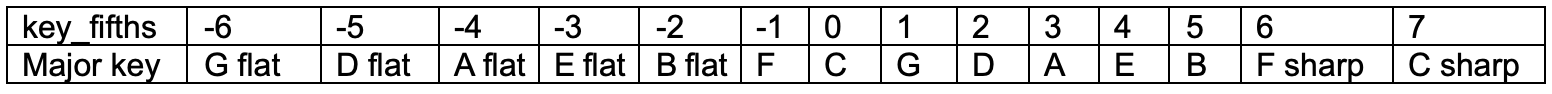
\includegraphics{Figures/key_fifths_mapping}
   % \decoRule
   % \caption{Mapping of \emph{key\_fifths} to major key}
   % \label{fig:kf_map}
    %\end{figure}

    \begin{table}
        \caption{Mapping of \emph{key\_fifths} to major key}
        \label{tab:kf_map}
        \centering
        \begin{tabular}{|c||c|c|c|c|c|c|c|c|c|c|c|c|c|c|}
        \hline
        \emph{key\_fifths} & -6 & -5 & -4 & -3 & -2 & -1 & 0 & 1 & 2 & 3 & 4 & 5 & 6 & 7 \\
        \hline
        Major key & Gb & Db & Ab & Eb & Bb & F & C & G & D & A & E & B & F\# & C\# \\
        \hline
        \end{tabular}
        \end{table}

\begin{table}
    \caption{Mapping of music notes to numerical representations}
    \label{tab:note_map}
    \centering
    \begin{tabular}{|c|c|c|c|c|c|}
    \hline
    C/B\# & C\#/Db & D & D\#/Eb & E/Fb & F/E\# \\
    \hline
    1 & 2 & 3 & 4 & 5 & 6 \\
    \hline
    \end{tabular}
    \begin{tabular}{|c|c|c|c|c|c|}
        \hline
    F\#/Gb & G & G\#/Ab & A & A\#/Bb & B/Cb\\
    \hline
    7 & 8 & 9 & 10 & 11 & 12\\
    \hline
    \end{tabular}
    \end{table}

    \begin{table}
        \caption{The component notes/pitches of each major key}
        \label{tab:bigtable}
        \centering
        \begin{tabular}{|c||c|c|c|c|c|c|c|}
        \hline
        Major key & Pitch 1 & Pitch 2 & Pitch 3 & Pitch 4 & Pitch 5 & Pitch 6 & Pitch 7 \\
        \hline
        \hline
        C\# & 2 & 4 & 6 & 7 & 9 & 11 & 1 \\
        \hline
        F\# & 7 & 9 & 11 & 12 & 2 & 4 & 6\\
        \hline
        B & 12 & 2 & 4 & 5 & 7 & 9 & 11\\
        \hline
        E & 5 & 7 & 9 & 10 & 12 & 2 & 4\\
        \hline
        A & 10 & 12 & 2 & 3 & 5 & 7 & 9\\
        \hline
        D & 3 & 5 & 7 & 8 & 10 & 12 & 2\\
        \hline
        G & 8 & 10 & 12 & 1 & 3 & 5 & 7\\
        \hline
        C & 1 & 3 & 5 & 6 & 8 & 10 & 12\\
        \hline
        F & 6 & 8 & 10 & 11 & 1 & 3 & 5\\
        \hline
        Bb & 11 & 1 & 3 & 4 & 6 & 8 & 10\\
        \hline
        Eb & 4 & 6 & 8 & 9 & 11 & 1 & 3\\
        \hline
        Ab & 9 & 11 & 1 & 2 & 4 & 6 & 8\\
        \hline
        Db & 2 & 4 & 6 & 7 & 9 & 11 & 1\\
        \hline
        Gb & 7 & 9 & 11 & 12 & 2 & 4 & 6\\
        \hline
        \end{tabular}
        \end{table}

        \begin{table}
            \caption{Mapping of chords present within the dataset to major/minor chord.}
            \label{tab:chords}
            \centering
            \begin{tabular}{l l}
            \toprule
            Major & Minor \\
            \midrule
            Dominant-ninth & Minor-seventh\\
            Major-sixth & Minor-sixth\\
            Major-seventh & Diminished\\
            Dominant & Half-diminished\\
            Suspended-fourth & Minor-ninth\\
            Augmented-seventh & Diminished-seventh\\
            Major-ninth & Minor-eleventh\\
            Dominant-seventh & Minor-major\\
            Augmented & Major-minor\\
            Dominant-thirteenth & Minor-thirteenth\\
            Power & Minor seven flat five\\
            Suspended-second &  \\
            Dominant-eleventh &  \\
            Pedal &  \\
            Major 6/9 &  \\
            Augmented-ninth &  \\
            Sixth &  \\

            \bottomrule\\
            \end{tabular}
            \end{table}
            

        \begin{figure}
            \centering
            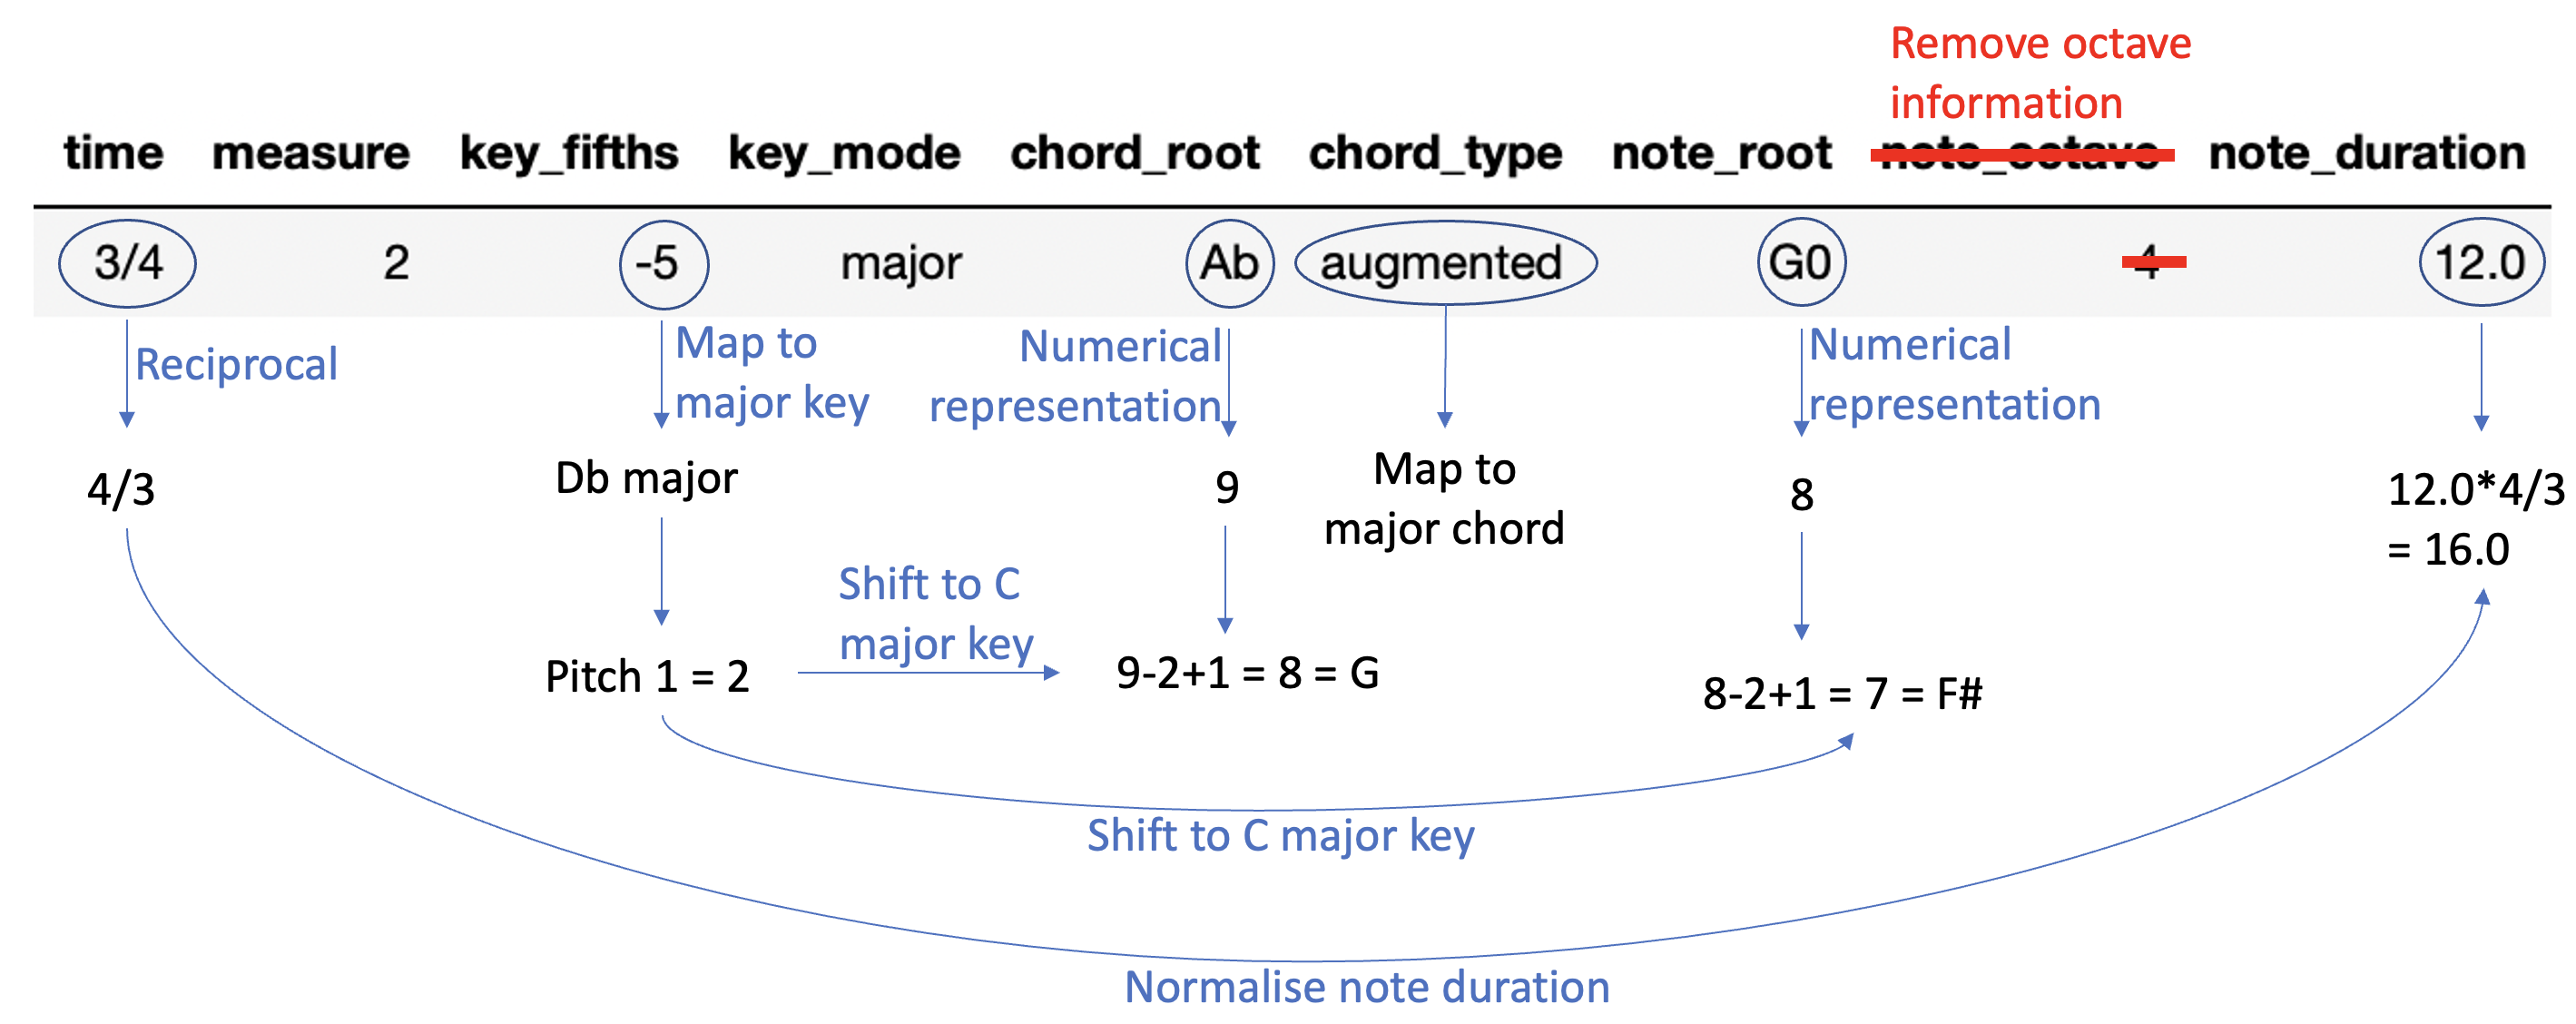
\includegraphics[scale=0.3]{Figures/Algorithm pictorial2}
            \decoRule
            \caption{Pictorial representation of the preprocessing of the dataset.
            }
            \label{fig:Alg1}
            \end{figure}
            
%-----------------------------------
%	SUBSECTION 2
%-----------------------------------

%\subsection{Subsection 2}
%Morbi rutrum odio eget arcu adipiscing sodales. Aenean et purus a est pulvinar pellentesque. Cras in elit neque, quis varius elit. Phasellus fringilla, nibh eu tempus venenatis, dolor elit posuere quam, quis adipiscing urna leo nec orci. Sed nec nulla auctor odio aliquet consequat. Ut nec nulla in ante ullamcorper aliquam at sed dolor. Phasellus fermentum magna in augue gravida cursus. Cras sed pretium lorem. Pellentesque eget ornare odio. Proin accumsan, massa viverra cursus pharetra, ipsum nisi lobortis velit, a malesuada dolor lorem eu neque.

%----------------------------------------------------------------------------------------
%	SECTION 3
%----------------------------------------------------------------------------------------

\section{Model input format}
Now that the dataset has been preprocessed, it can now be converted into a format that is appropriate for input to the machine learning model. Since we are focusing on the LSTM and the Transformer, we will have to convert the data into formats that are appropriate for those two models.

\subsection{LSTM format}
\label{LSTM format for training}
The LSTM data input format is a matrix with 37 columns, with each row containing informaion about a single measure. The first 12 columns represent the 12 note (C,C\#, etc.), the next 24 columns represent the 12 major chords and the 12 minor chords, and the last column correspond to the absence of a chord. If a particular note exists within a particular measure, the element that corresponds to that particular measure (row) and particular note (column) will be the normalised duration of that note. Similarly, the element that corresponds to the chord of a particular measure will be a '1'. Notes and chords that are not present within that measure will be marked with a '0'. If no chords are present within a measure, the last column will be marked as a '1'. A pictorial representation of the transformation is shown in Figure \ref{fig:LSTM training}.

\subsubsection{Code}
We again use a nested loop to loop through each DataFrame row for each song. Two 1 by 37 arrays \emph{LSTM\_data} and \emph{new\_row} are initialised. As we loop through each row, we keep track of the meaasure. As long as the measure does not change, \emph{new\_row} is progressively updated with the normalised note durations of the present notes in this manner: 
\begin{equation}  
\emph{new\_row}[0,\emph{note}-1] = \emph{new\_row}[0,\emph{note}-1] + \emph{normalised\_note\_duration},
\end{equation}
where \emph{note} is the numerical representation of the note present in each DataFrame row and \emph{normalised\_note\_duration} is the normalised note duration of that note. 

This works because the mapping between the notes and their numerical representation starts at 1 and ends at 12 (as can be seen in Table \ref{tab:note_map}) and indexing starts at zero in Python. Hence, the (\emph{note}-1)\textsuperscript{th} column of the LSTM format (and thereby \emph{new\_row}) will correspond to \emph{note}.

Once the measure changes, the now complete \emph{new\_row} for the previous measure is concatenated with \emph{LSTM\_row} along the row axis, i.e. \emph{new\_row} is added to the bottom of \emph{LSTM\_row}. The elements of \emph{new\_row} are reset to zero before \emph{new\_row} is updated with the note and chord information of the current measure. The note information can be updated as explained earlier. For the chord information, we can use \emph{if} statements to set $\emph{new\_row}[0, \emph{chord}+11] = 1$ if \emph{chordtype} = 'major', or to set $\emph{new\_row}[0, \emph{chord}+23] = 1$ if \emph{chordtype} = 'minor', or to set $\emph{new\_row}[0, -1] = 1$ otherwise (no chord present), where \emph{chord} is the numerical representation of \emph{chord\_root} (mapped using Table \ref{tab:note_map}). Since we know that there is only one chord type per measure, we only have to update the chord information for \emph{new\_row} once, at the start of a new measure. The start of the first measure can be taken to be a special case of a measure change (in this case, transition from a measure initialised as 'unknown' to the first measure of the DataFrame).

Note that we could have combined this section with the preprocessing steps in Chapter \ref{preprocessing} such that we only have to loop through each DataFrame row for each song once instead of doing it twice as we actually did. This would have reduced the time needed to run the entire code by eliminating redundant loops. However, the time saved for a dataset of this size is insignificant. Additionally, keeping the two code blocks separate made it easier to test and debug, which is why we decided not to integrate them together. Nonetheless, integration of the code is definitely something to take into consideration for any future extensions of this project.
%$\emph{new\_row}[0,\emph{note}-1] = \emph{new\_row}[0,\emph{note}-1] + \emph{normalised\_note\_duration}$
\begin{figure}
    \centering
    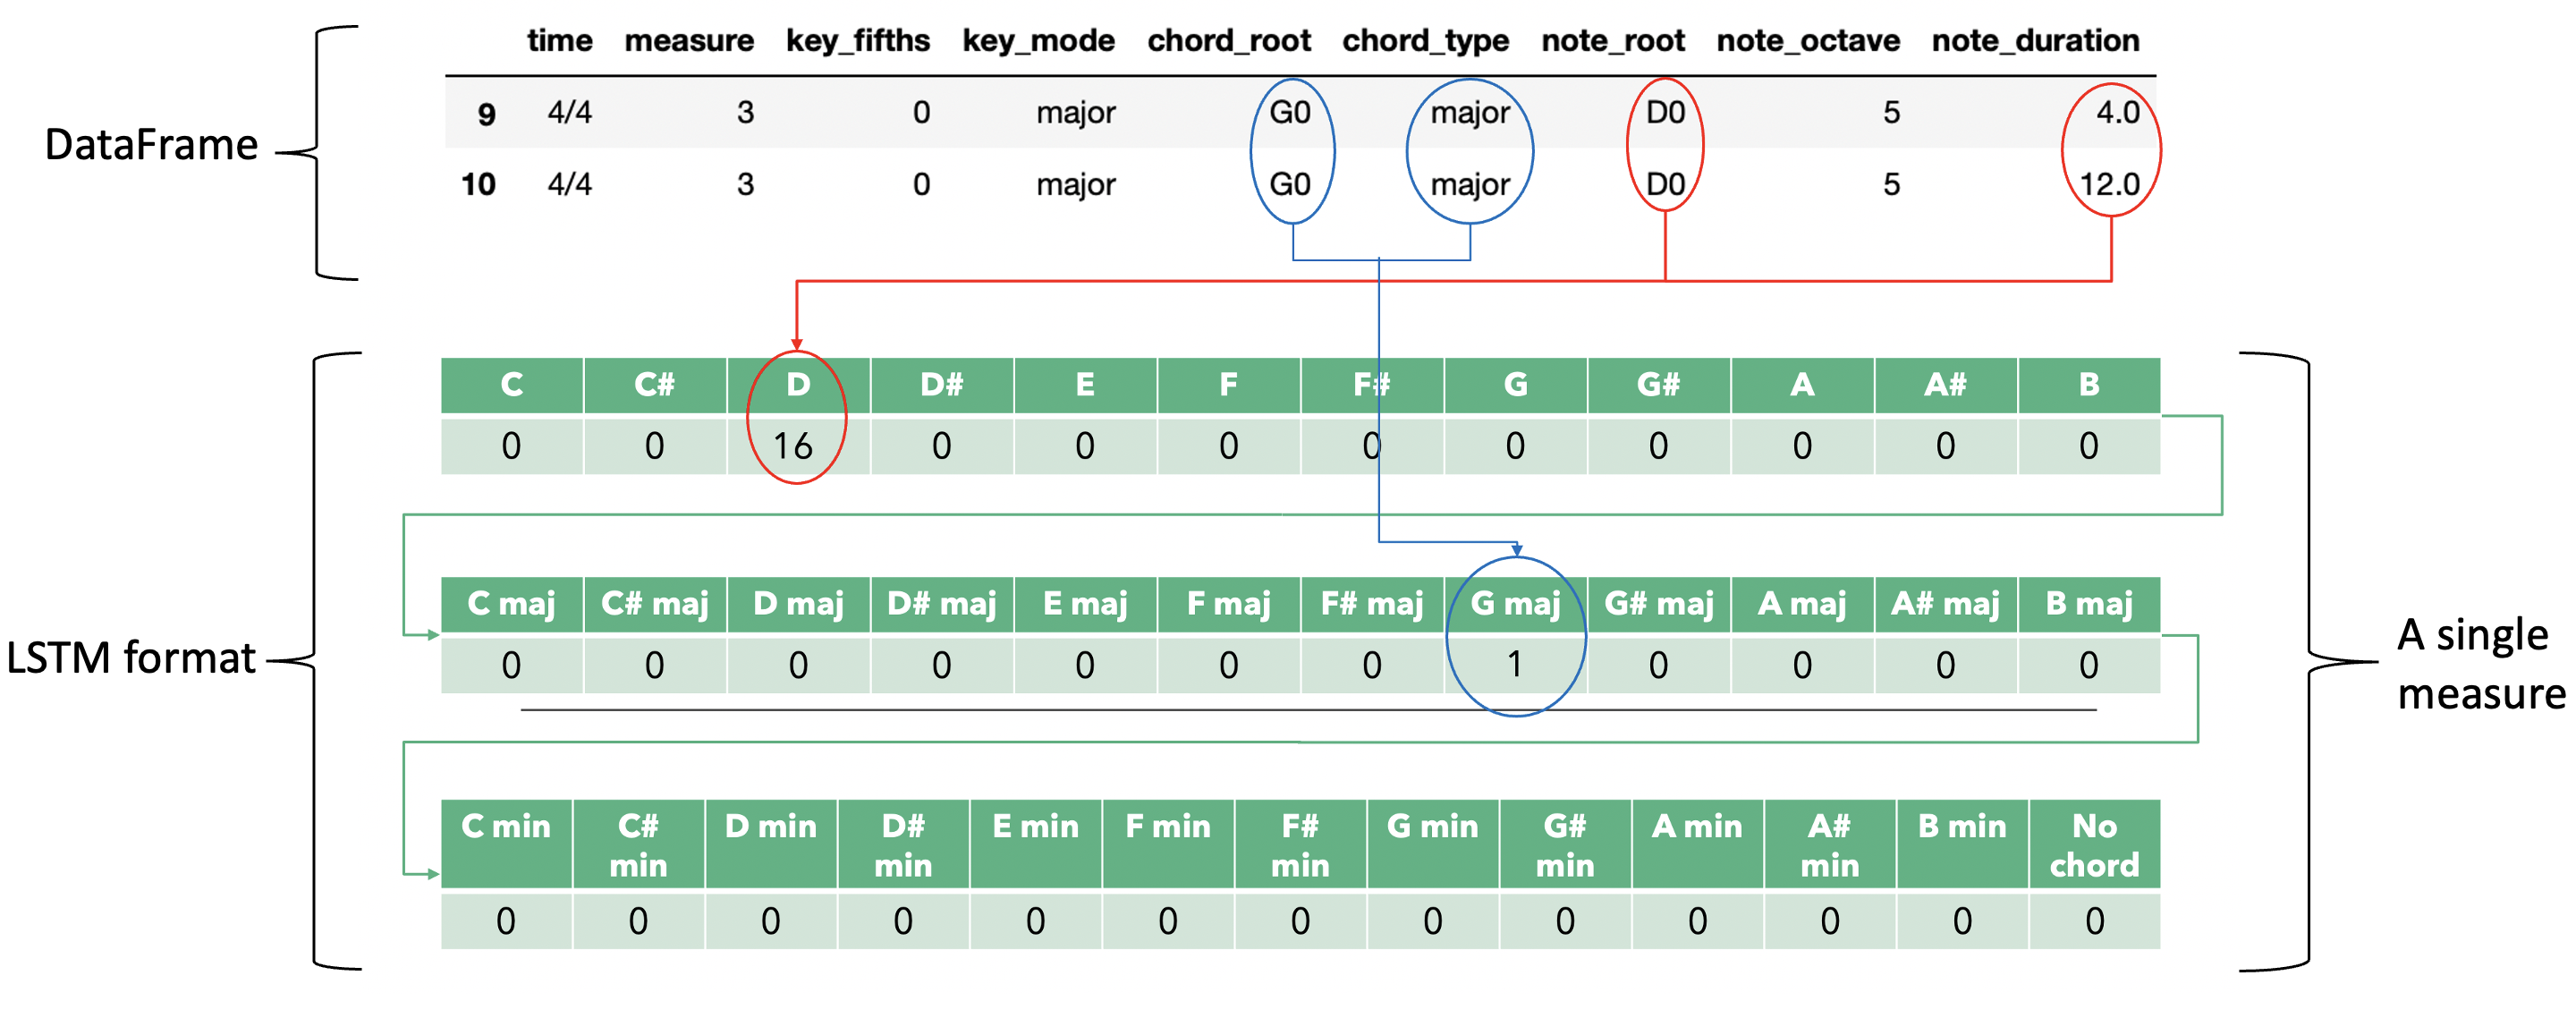
\includegraphics[scale=0.3]{Figures/LSTM pictorial 4}
    \decoRule
    \caption{Transforming DataFrame to LSTM data input format.}
    \label{fig:LSTM training}
    \end{figure}
    
\subsubsection{Sanity Check of code}
\label{lstm check}
We know that each row of the LSTM data input format corresponds to a single measure. We also know that the preprocessing done in Chapter \ref{preprocessing} would have removed unnecessary measures from some songs. Hence, the LSTM data cannot possibly have more measures than the original dataset for each song. By comparing the number of rows of the LSTM data and the highest value of \emph{measure} in the original Dataframe for each song, we can perform a simple check of the correctness of our code. From Figure \ref{fig:LSTM check}, we can see that no songs in LSTM data input format has more measures than in their original DataFrame format.

In addition, we picked out a few songs at random and manually checked the format conversion.

\begin{figure}
    \centering
    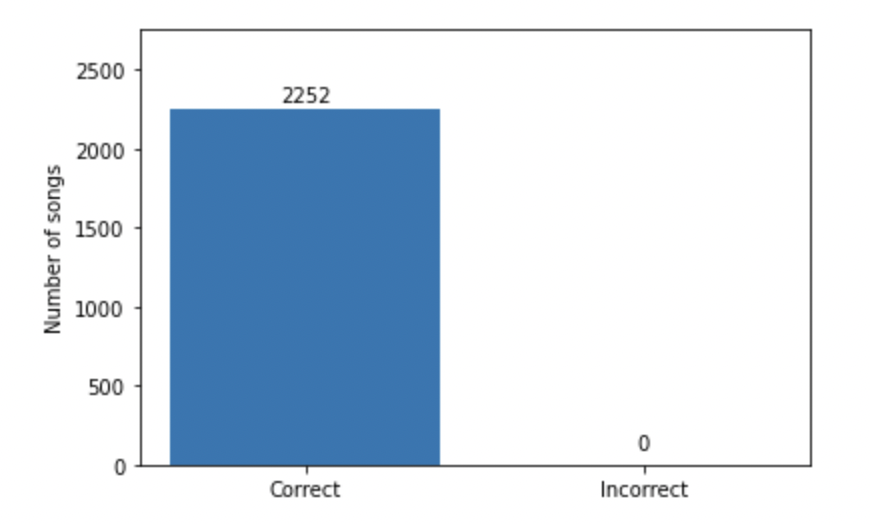
\includegraphics{Figures/LSTM check}
    \decoRule
    \caption{Number of songs in LSTM format with 'correct' and 'incorrect' number of measures.}
    \label{fig:LSTM check}
    \end{figure}

\subsection{Transformer format}
\label{Transformer format for training}
The transformer requires two data inputs: a single sequence of notes for each song, and a separate sequence of chords for each song. Both sequences are constructed by going down the Dataframe rows, and adding the notes/chords of each row to the respective sequences based on the \emph{note\_duration} value, e.g. a sequence of 4 'C\#'s for a 'C\#' with a \emph{note\_duration} of 4.0, and a sequence of 16 'Bmaj's for a 'B major' of \emph{note\_duration} of 16.0. Another example is presented in Figure \ref{fig:Transformer training}. This means that only integer values of \emph{note\_duration} are accepted and measures with non-integer values have to be removed beforehand.

It is obvious that the sequences will be very long given that just the three rows in Figure \ref{fig:Transformer training} resulted in 16 elements for each sequence. As shown in Chapter 4, the time complexity of the Transformer is $O({n}^2)$. Hence, it is crucial to reduce the sequence length to shorten the training time. This can be achieved by dividing all \emph{note\_duration} by their largest common factor for all measures within a single song. This may not reduce the length of the sequences for all songs (songs with \emph{note\_duration of 1.0} will have a trivial largest common factor of 1.0), but it will still reduce the sequence length for some songs, as shown in Figure \ref{fig:Transformer LCF}, which will decrease the training time significantly.


\begin{figure}
    \centering
    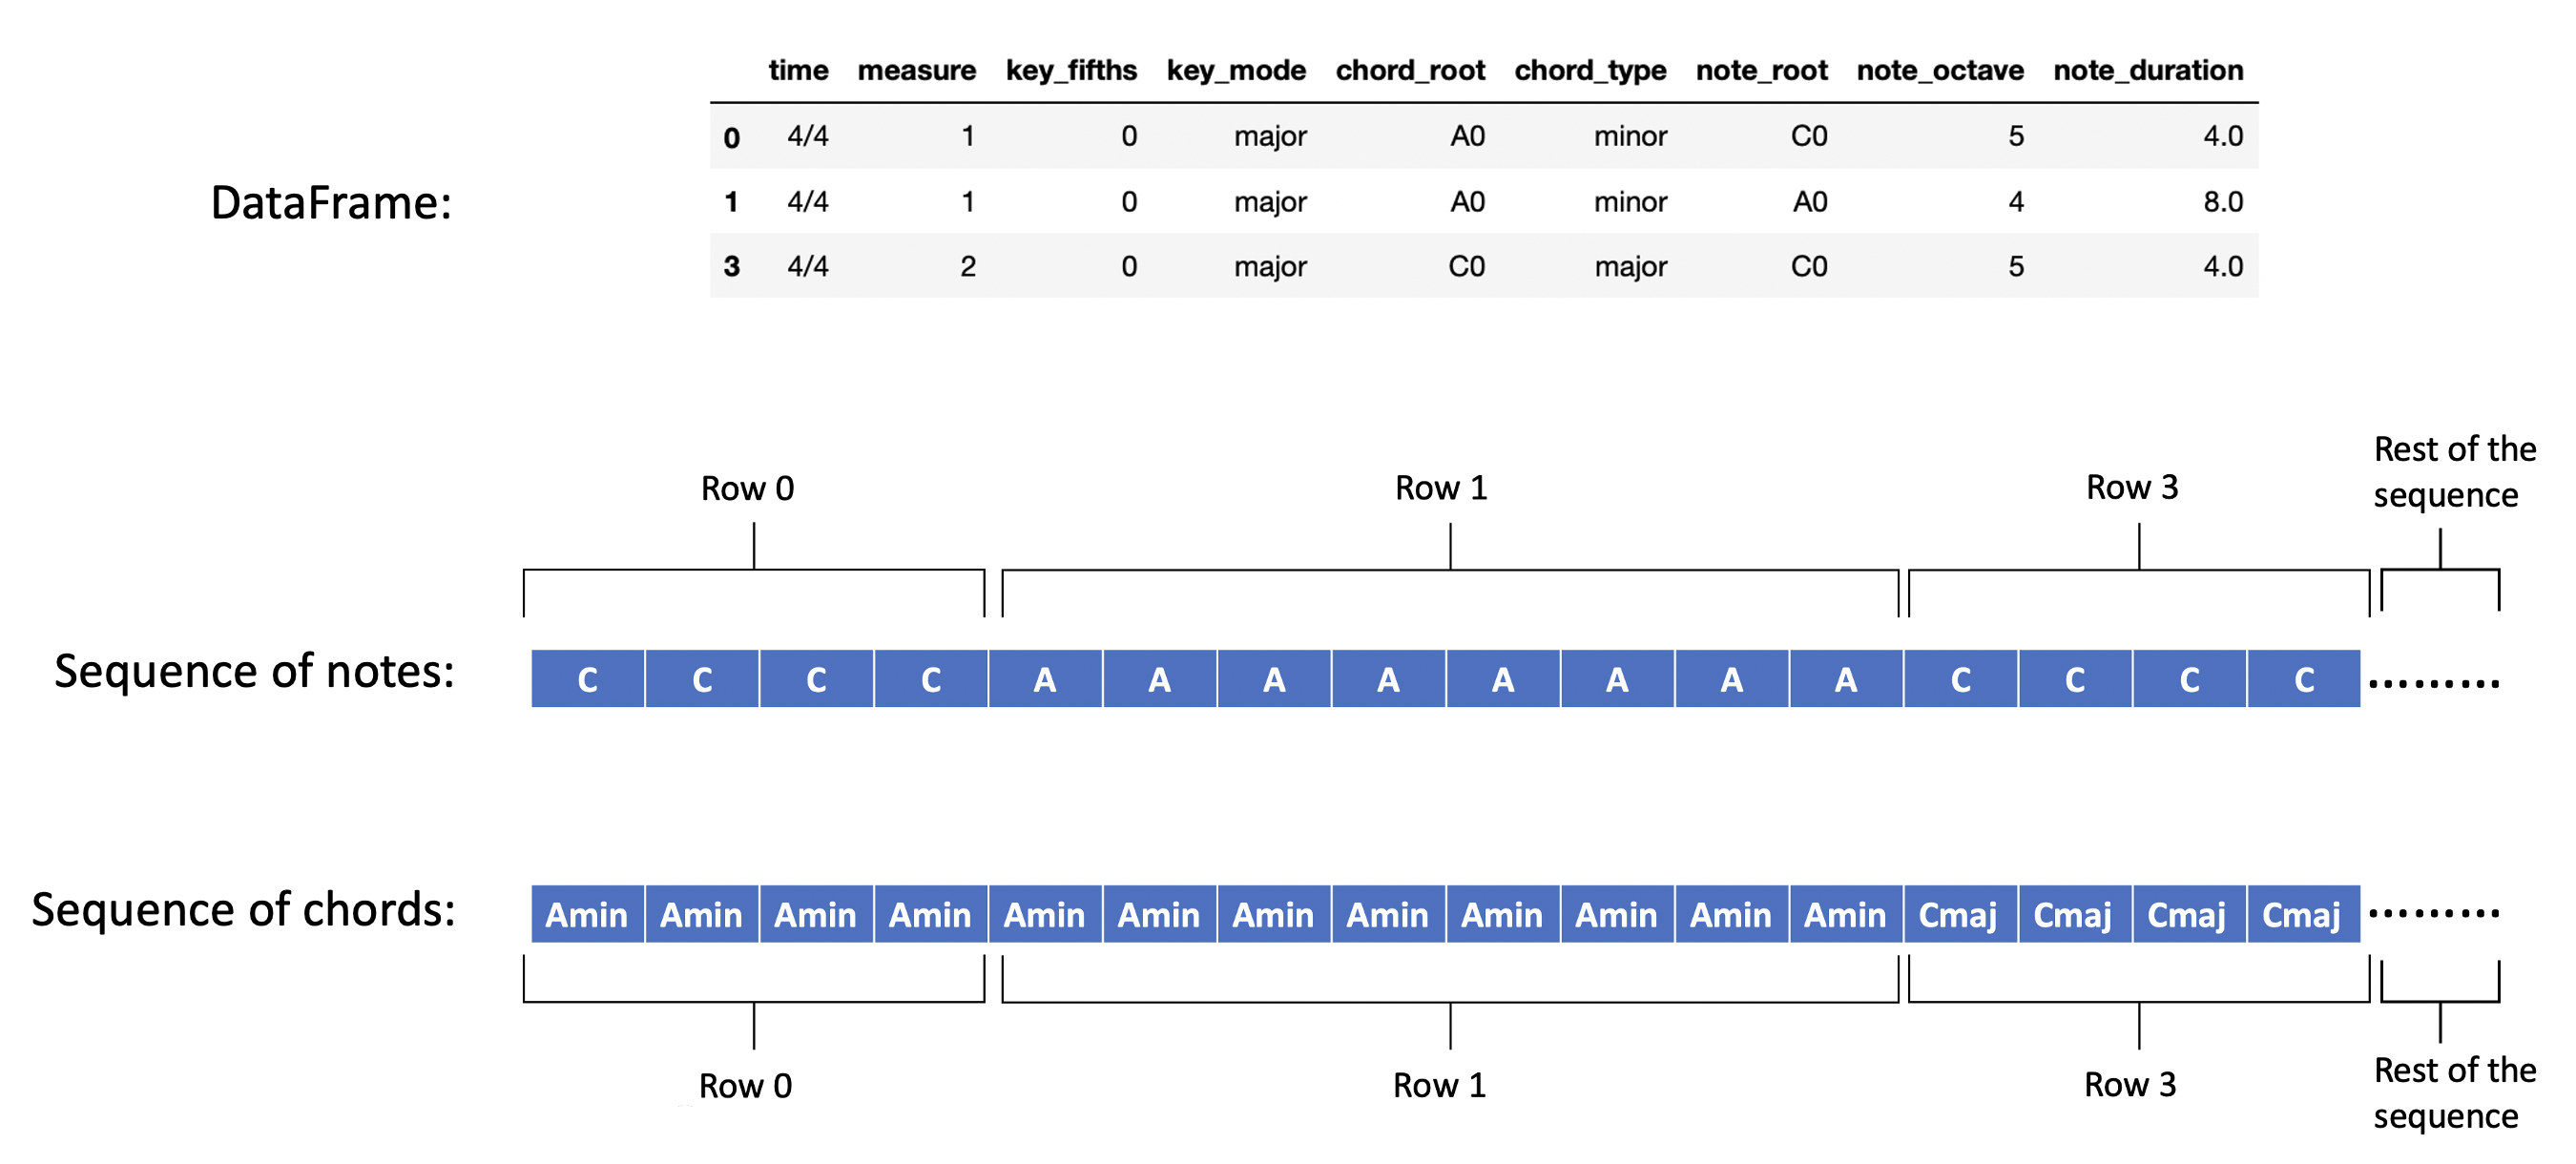
\includegraphics[scale=0.3]{Figures/TransformerData}
    \decoRule
    \caption{Converting DataFrame to Transformer data input format.}
    \label{fig:Transformer training}
    \end{figure}

\begin{figure}
    \centering
    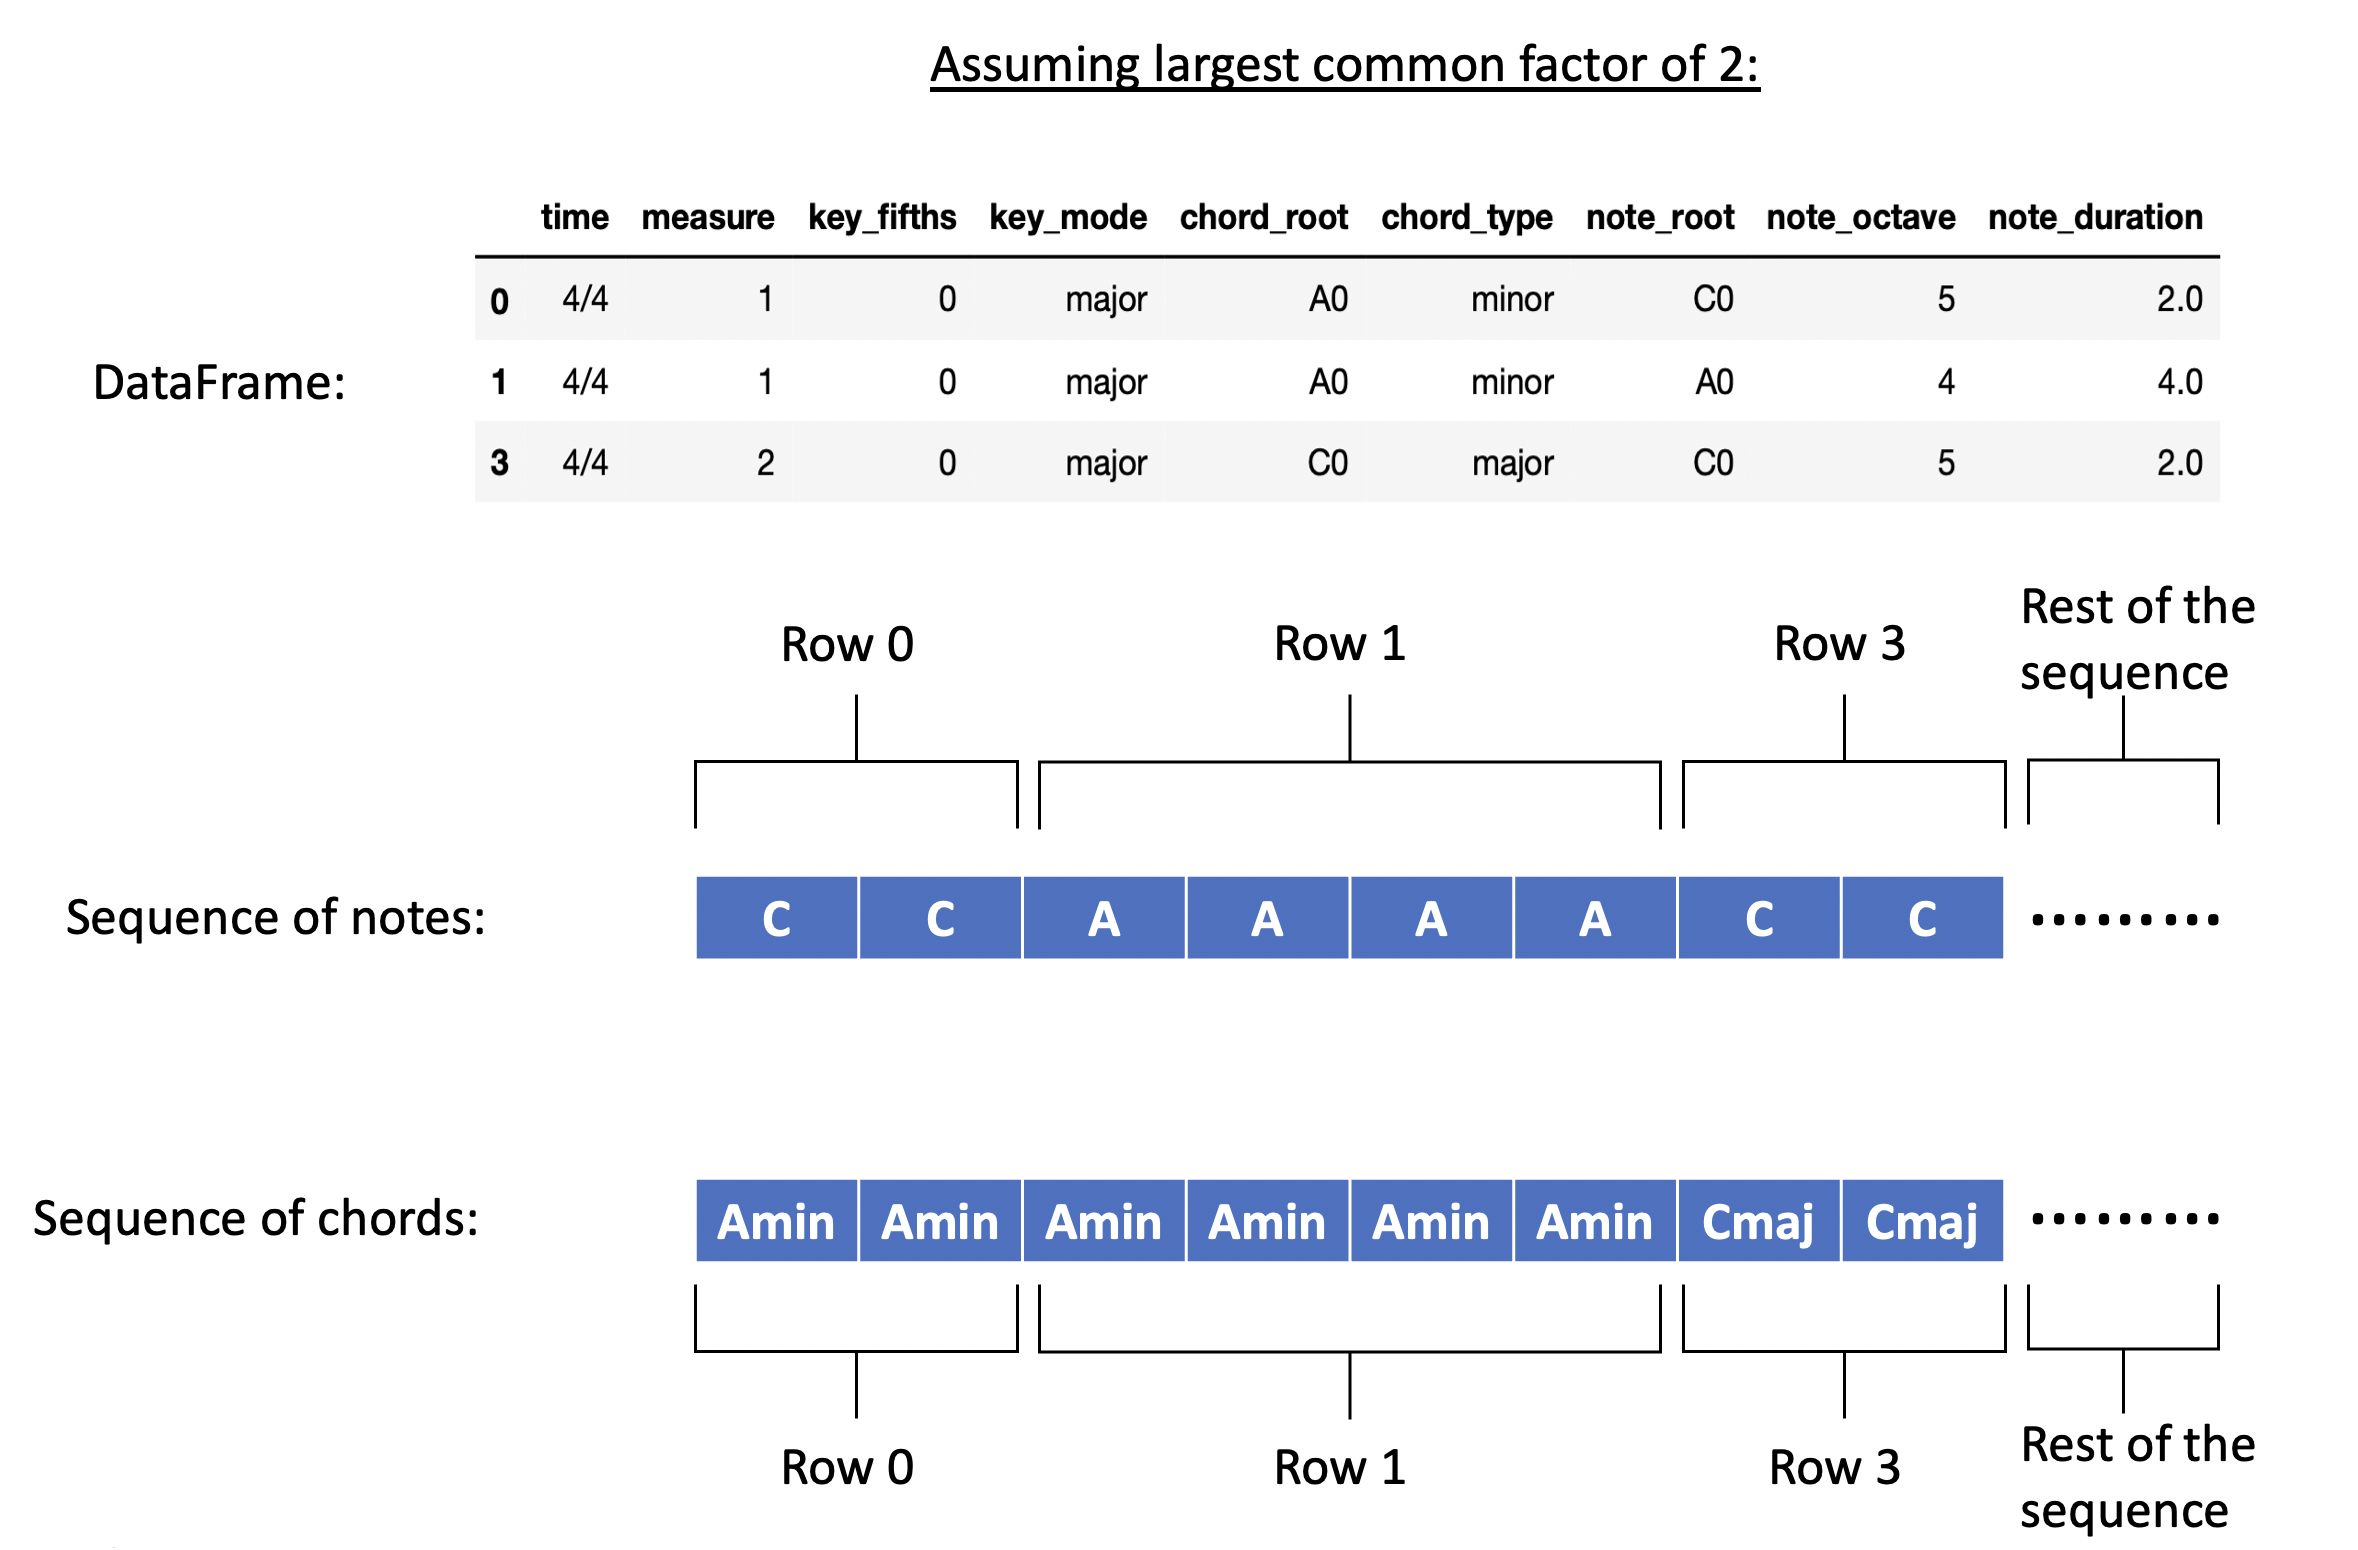
\includegraphics[scale=0.3]{Figures/Transformer LCF}
    \decoRule
    \caption{Converting DataFrame (normalised by the largest common factor) to Transformer data input format.}
    \label{fig:Transformer LCF}
    \end{figure}

\subsubsection{Code}
The same nested loop as before is used again for this. Four empty lists \emph{note\_duration\_li}, \emph{note\_li}, \emph{chord\_li}, \emph{chordtype\_li} are initialised. As we loop through the DataFrame rows of a single song, we append the information from each row to the respective lists. At the end of this inner loop, the largest common factor of \emph{note\_duration\_li} can be found using the \emph{math.gcd} function:

\begin{lstlisting}[language=Python]
    lcf = note_duration_li[0]   #Initialise lcf
    n = len(note_duration_li)   #Number of elements in list
    
    for j in range(1,n):
        lcf = math.gcd(lcf,note_duration_li[j])
\end{lstlisting}


Since \emph{math.gcd} only accepts two arguments, we initialise \emph{lcf} as the index 0 element of \emph{note\_duration\_li}, and loop from the index 1 element to the last element of \emph{note\_duration\_li}. Within this loop, \emph{math.gcd} takes in \emph{lcf} and \emph{note\_duration\_li}[\emph{j}] as its two arguments, where \emph{j} is the correct loop index. In essence, we are just finding the largest common factor of the first two elements of \emph{note\_duration\_li}, and finding the largest common factor of the previous largest common factor and the third element, and so on. This will give us the largest common factor of all the values stored in \emph{note\_duration\_li}, which are all then divided by this largest common factor to give \emph{normalised\_note\_duration}.

We can now start to construct the sequences of notes and chords. Two empty arrays \emph{row\_note} and \emph{row\_chord} are initialised, and we loop through \emph{normalised\_note\_duration} with loop index \emph{k}. For the \emph{k}\textsuperscript{th} element of \emph{normalised\_note\_duration}, a 1 by \emph{normalised\_note\_duration}[\emph{k}] array filled with '1's is initialised and multiplied by \emph{note\_li}[\emph{k}]. The result is concatenated with \emph{row\_note} along the column axis. For the chord sequence, a 1 by \emph{normalised\_note\_duration}[\emph{k}] array filled with '1's is also initialised. This array is multiplied by \emph{chord\_li}[\emph{k}] if chordtype\_li[\emph{k}] is 'major', by $(\emph{chord\_li}[\emph{k}] + 12)$ if it is 'minor', and zero if there are no chords. The resulting array is then concatenated with \emph{row\_chord} along the column axis.

After looping through all the DataFrame rows of a song, \emph{row\_note} and \emph{row\_chord} are the now complete sequences of notes and chords respectively for that song. These will be the input to the Transformer model.

\subsubsection{Sanity Check of code}
We expect the number of elements in each of the note/chord sequence to be less than or equal to the sum of all \emph{note\_duration} for a single song. It will be 'less than' if all the \emph{note\_duration}s have a largest common factor greater than 1.0. Indeed, we see that this is the case for all 4504 note/chord sequences (twice the number of songs in the dataset since we are splitting each song into a separate note and chord sequence) in Figure \ref{fig:Transformer check}.

Again, we manually check a random selection of sequences like we did in the sanity check for the LSTM in Chapter \ref{lstm check}.

\begin{figure}
    \centering
    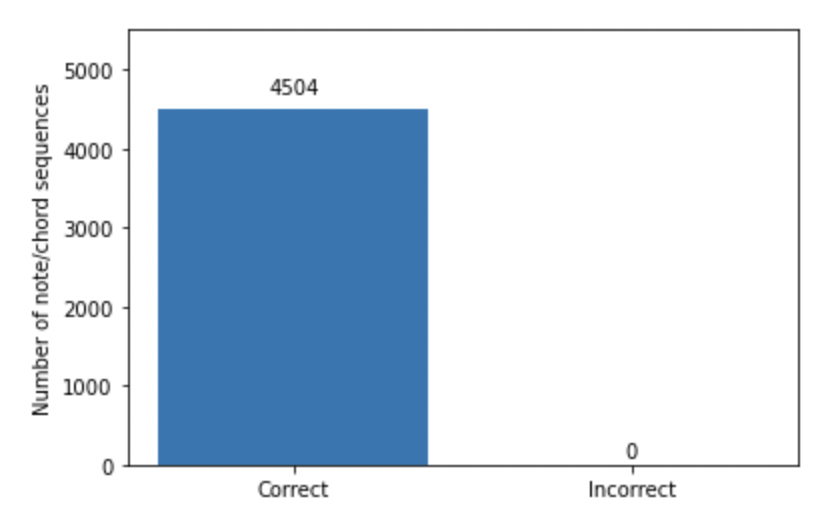
\includegraphics{Figures/Transformer check}
    \decoRule
    \caption{Number of note/chord sequences with 'correct' and 'incorrect' number of columns.}
    \label{fig:Transformer check}
    \end{figure}


\section{Data processor}
\label{data processor}
The data processor receives three pieces of information from the voice processor: note, music key, and note duration. Hence, the preprocessing needed is similar to the one in Section \ref{preprocessing} but simplified.

\begin{enumerate}
    \item Convert the notes to their numerical representations using Table \ref{tab:note_map} to obtain $n_r$.
    \item Since we have the music key information, we can find Pitch 1 of that key using Table \ref{tab:bigtable} to obtain $p_1$.
    \item We now have $n_r$ and $p_1$ and can use Equation \ref{shift note 2} to transpose the notes to C major key.
    %\item Normalise the time signatures by multiplying each note duration with the reciprocal of the time signature to give a normalised note duration.
    \item The preprocessed information is then converted into the LSTM or Transformer format. Note that we needed to provide the chord information to the model when training it, but once trained, the model is meant to output the chords themselves in actual operation. Hence, the data format for the data processor will differ from the data format for the training phase in that the former will only include note information and not chord information.
    \item The fully processed input data is passed to the machine learning model.
  \end{enumerate}

  \subsection{LSTM format}
Since the chord information is no longer needed, the last 25 columns are now irrelevant. Hence, the input data is just a matrix with 12 columns as shown in Figure \ref{fig:LSTM data processor}. Notice the difference between Figure \ref{fig:LSTM data processor} and Figure \ref{fig:LSTM training}.

\begin{figure}
    \centering
    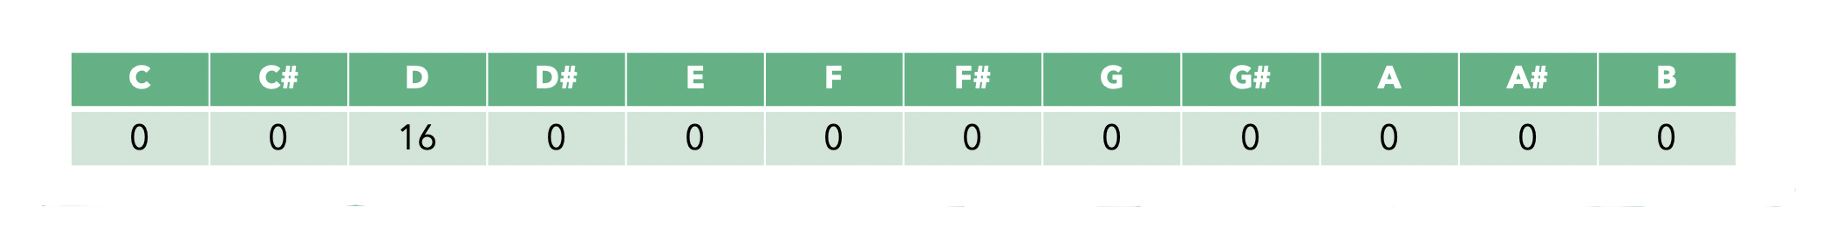
\includegraphics[scale=0.3]{Figures/LSTM data processor}
    \decoRule
    \caption{LSTM data input format (for a single measure) for data processor}
    \label{fig:LSTM data processor}
    \end{figure}

\subsection{Transformer format}
Similarly, we no longer have a sequence of chords since the chord information is presumably not known. This just leaves the sequence of notes, as shown in Figure \ref{fig:Transformer data processor}. Note the difference between Figure \ref{fig:Transformer data processor} and Figure \ref{fig:Transformer LCF}.

\begin{figure}
    \centering
    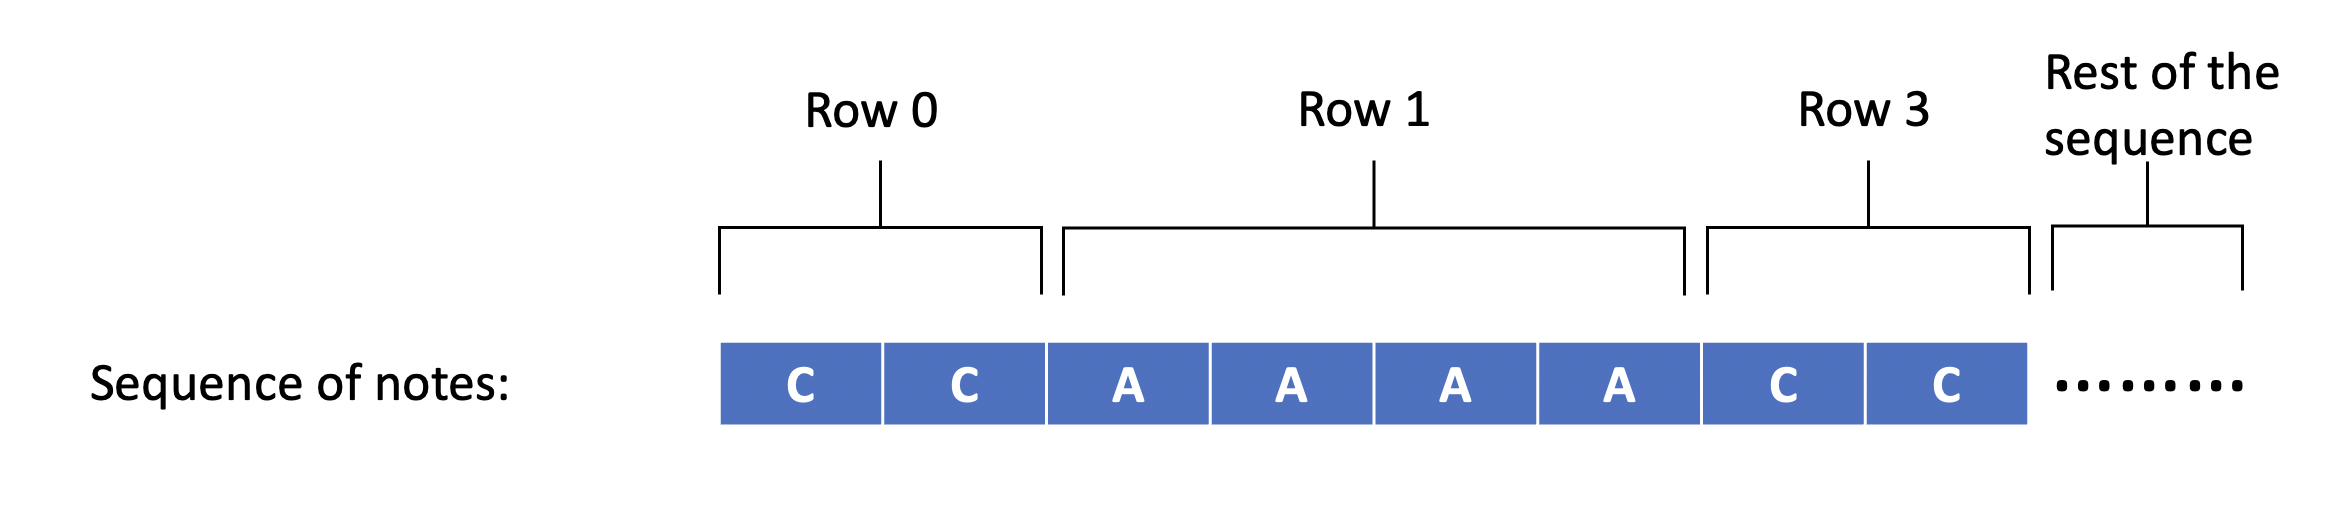
\includegraphics[scale=0.3]{Figures/Transformer data processor}
    \decoRule
    \caption{Transformer data input format for data processor}
    \label{fig:Transformer data processor}
    \end{figure}

\section{Music Mood Classification}
Everything dicussed above in this chapter is crucial to the creation of our Minimum Viable Product. However, there are additional features that we could add to our product if it proves to be successful. One possible additional functionality would be allowing users to select the music mood of the generated chords, or perhaps even have our machine learning model be able to identify the mood of their singing. This means that our model would need to be trained to identify music moods, which would require mood information in the training dataset. While datasets with expert annotations of music moods exist \cite{allmusic}, it would be useful to be able to assign a music mood to a song ourselves using some sort of algorithm or model.

%\subsection{Human annotations}

%\subsection{Machine learning model annotations}

Classifying the music mood of songs using machine learning models has been a prominent problem in the Music Informatics Research (MIR) community for years \cite{MIRMood}. There are generally two approaches to this problem: regressing a continuous mood space, or treating it as a multi-label classificaiton problem. The latter seems to perform better when working with listener data rather than just the audio content \cite{ListeningData}. Unfortunately, listener data would be difficult to obtain as it is valuable information that corporations would be unlikely to divulge. Additionally, our model will mainly be dealing with newly created song for which listener data will not be available. Hence, an audio-based approach will be our only option if we are to use a machine learning model for mood classification. This leaves us with the continuous mood space.

%\subsubsection{Continuous mood space}

The continuous mood space can be regressed and then clustered to obtain specific moods. This would require an appropriate continuous mood space model.

First, we have the Arousal-Valence model \cite{circumplex}, which is a well-known model in the field of psychology and cognitive science \cite{circumplexbook} \cite{circumplex3}. This model displays emotions on a two-dimensional plane with valence (positive and negative degree of emotion) and arousal (intensity of emotion) as its two axes. Emotions are placed on the two-dimensional model based on their valence and arousal. This model is shown in Figure \ref{fig:circumplex}.

Next, we have Thayer's model, which applies the Arousal-Valence model to music. The main difference is the two axes, with Energy (the volume of the music) and Stress (tonality and tempo of the music) now corresponding to Arousal and Valence. Depending on the level of Energy and Stress, music can be classified into four clusters: Exuberance, Anxious, Contentment, and Depression. This model can be seen in Figure \ref{fig:Thayers}.

Lastly, we have the Tellegen-Watson-Clark model \cite{Watson1985} \cite{Tellegen1999}, which uses positive/negative affect, engagement/disengagement, and pleasantness/unpleasantness to classify music moods. This allows the model to classify a greater variety of music moods than the Arousal-Valence model and the Thayer's model. The Tellegen-Watson-Clark model is shown in Figure \ref{fig:TWC}.

Given that the it can classify the greatest variety of music moods, the Tellegen-Watson-Clark model would be the desired model should we decide to tackle the music mood classifiction problem with a continuous mood space approach. 

\begin{figure}
    \centering
    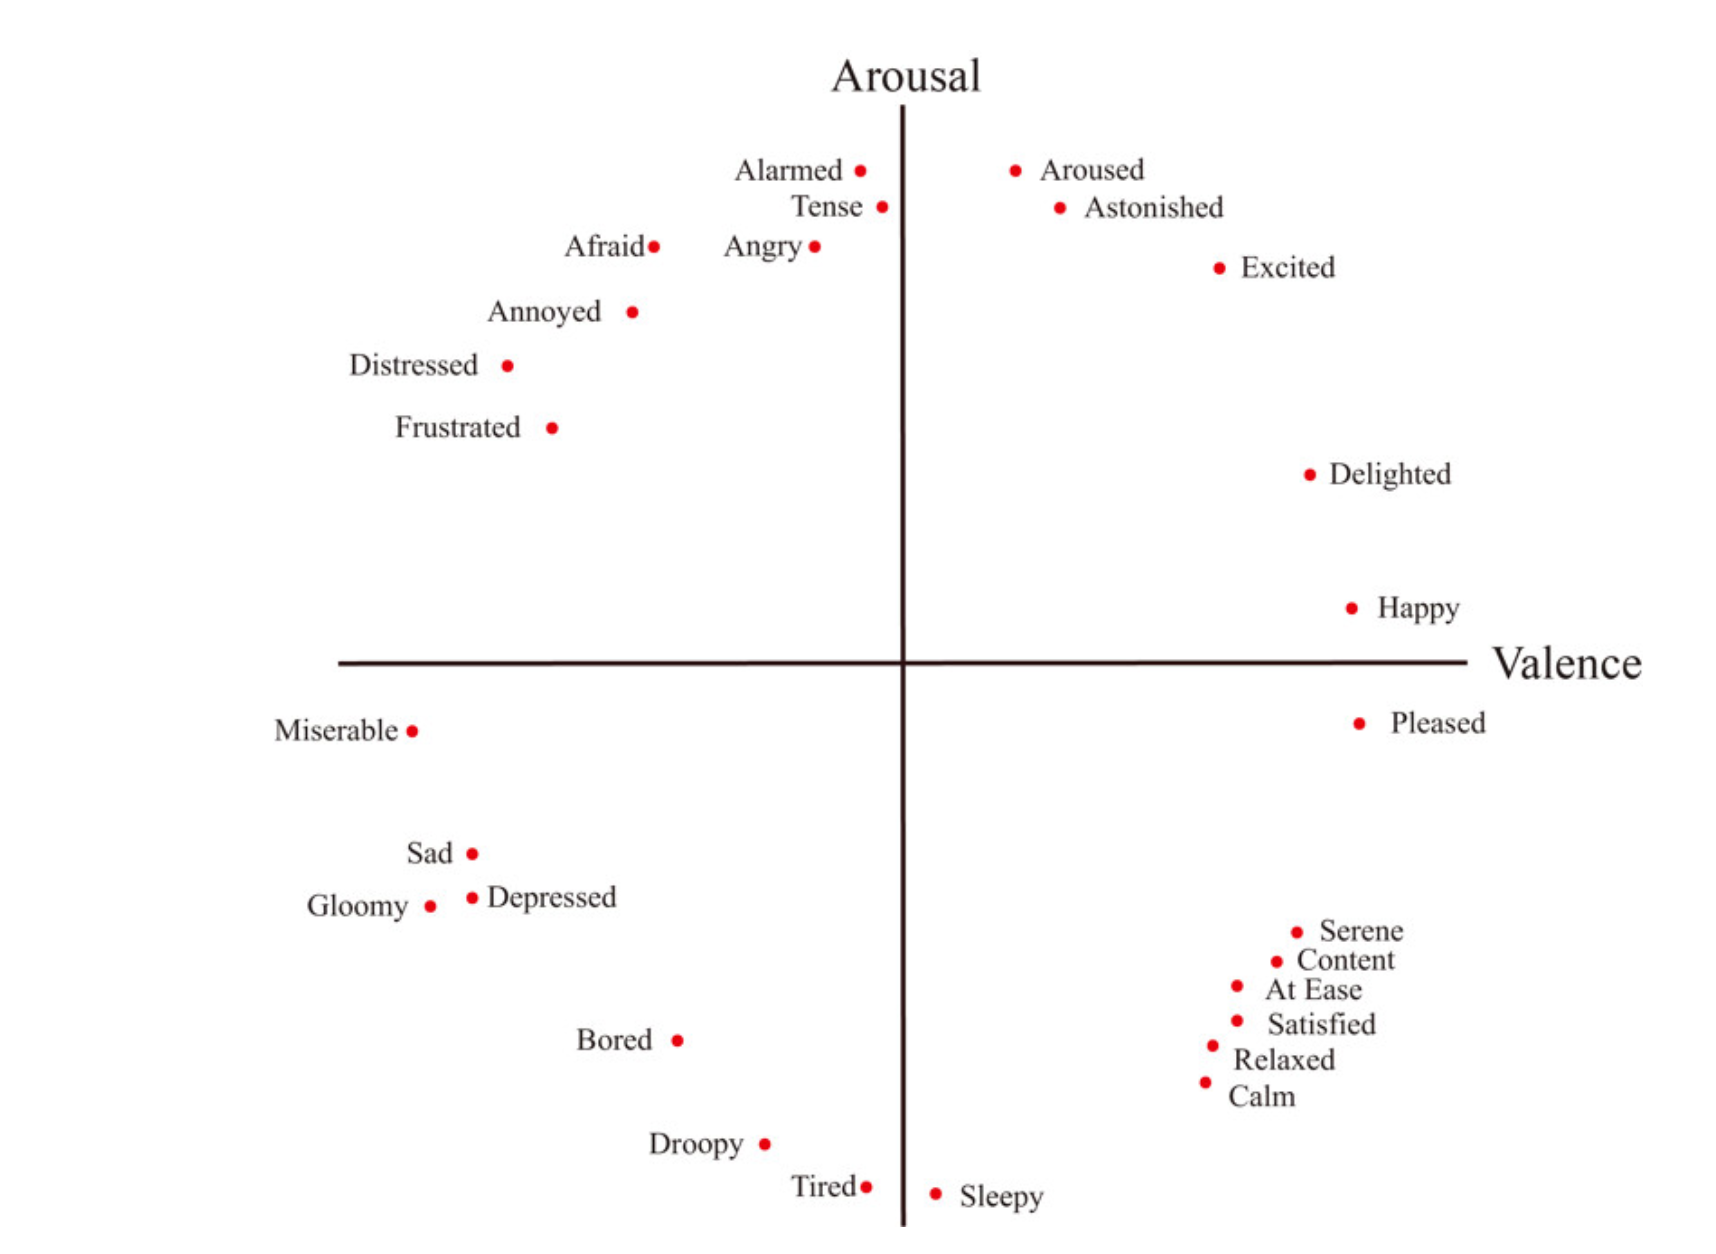
\includegraphics[scale=0.4]{Figures/Arousal-Valence model}
    \decoRule
    \caption{Arousal-Valence model \cite{MoodIoT}}
    \label{fig:circumplex}
    \end{figure}


\begin{figure}
    \centering
    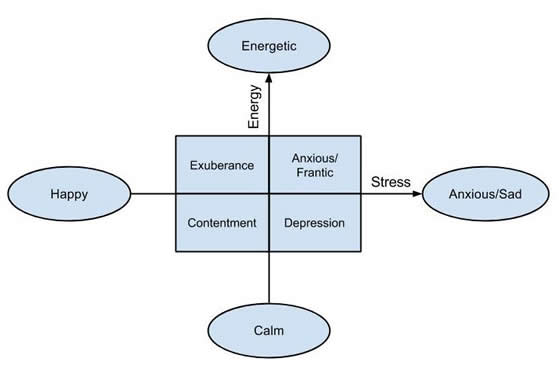
\includegraphics[scale=0.4]{Figures/Thayers model}
    \decoRule
    \caption{Arousal-Valence model \cite{MoodTufts}}
    \label{fig:Thayers}
    \end{figure}

\begin{figure}
    \centering
    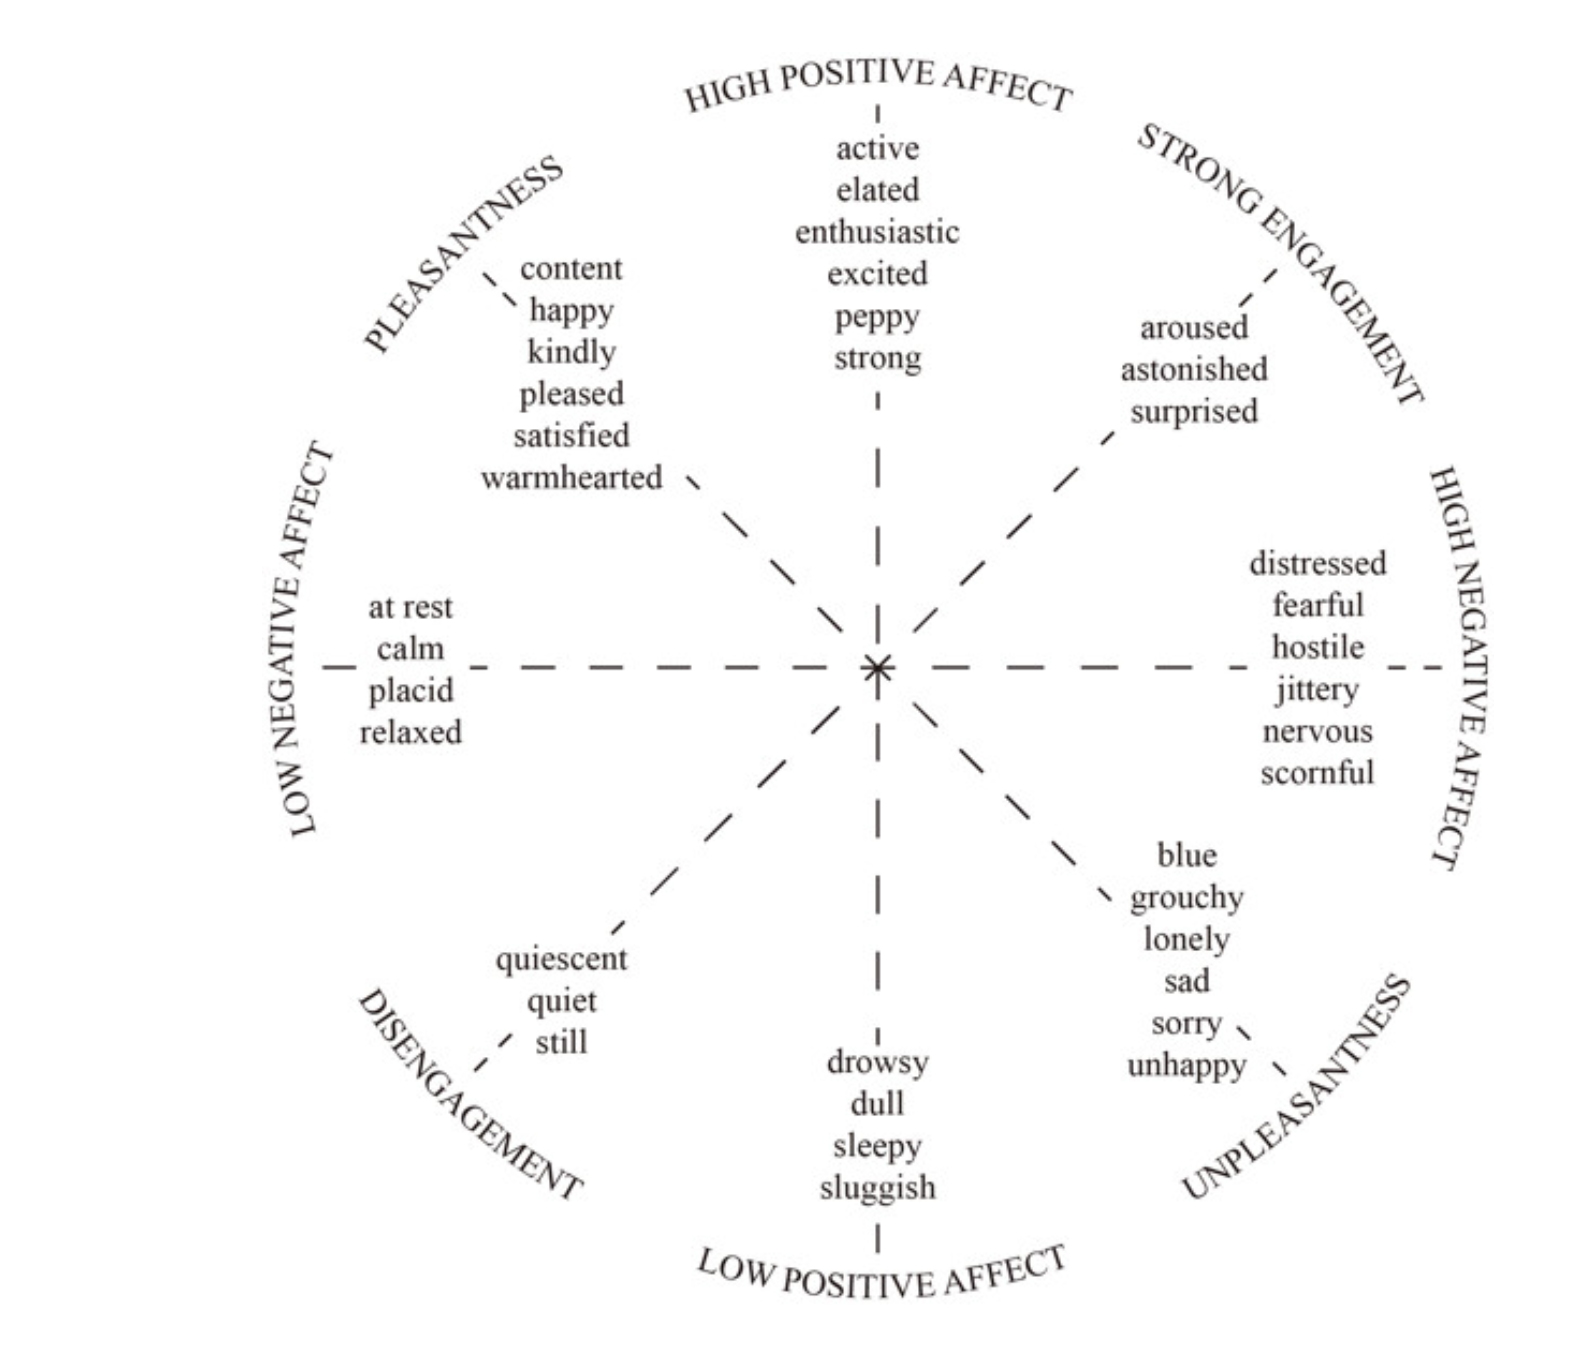
\includegraphics[scale=0.4]{Figures/TWC model}
    \decoRule
    \caption{Arousal-Valence model \cite{MoodIoT}}
    \label{fig:TWC}
    \end{figure}

As for the machine learning model, we would use a Support Vector Machine, which is a classification algorithm. When tested against other popular classification algorithms such as deep neural network /cite{MoodDeepNeuralNetwork}, random forest \cite{Moodrandomforest}, and K-nearest neighbour \cite{MoodKNeighbour} \cite{MoodDeepNeuralNetwork}, the Support Vector Machine was best at classifying music moods \cite{MoodIoT}.

% Chapter Template
\tocdata{toc}{Edward Gunn}

\chapter{Chord Generation Model} % Main chapter title
\chaptermark{Chord Generation Model - Edward Gunn}
\label{Chapter4} % Change X to a consecutive number; for referencing this chapter elsewhere, use \ref{ChapterX}

%----------------------------------------------------------------------------------------

% Define some commands to keep the formatting separated from the content 
\newcommand{\keyword}[1]{\textbf{#1}}
\newcommand{\tabhead}[1]{\textbf{#1}}
\newcommand{\code}[1]{\texttt{#1}}
\newcommand{\file}[1]{\texttt{\bfseries#1}}
\newcommand{\option}[1]{\texttt{\itshape#1}}

%----------------------------------------------------------------------------------------

%----------------------------------------------------------------------------------------
%	SECTION 1
%----------------------------------------------------------------------------------------

\section{Introduction}

We now move on to the inner workings of the model node from \cref{fig:MVPOverview}.
In order to find the relationship between the encoded melody processed in \cref{Chapter5} and \cref{Chapter3} we designed a machine learning model.
The dataset processed in \cref{Chapter3} is used to train and test this model to produce high quality accompaniment with knowledge of a variety of genres.
The problem of generation of a set of chords from a melody is very similar to that of translating one language to another. 
The translation problem is one that is very popular in machine learning research and thus there are many resources on it.  
However, the music related problem is harder to solve due to the extra dimension each of its elements contains. 
Each element in a melody has both pitch, represented by a discrete symbol or note, and duration whereas each element in the sequence of language is composed of only the discrete symbols or words.  
Therefore, in order to use techniques developed for natural language processing, it is necessary to encode the melody and chords in such a way that their dimensions are collapsed into one. 
Since this collapsing of dimensions has already been conducted in \cref{Chapter3} we are able to take full advantages of NLP techniques.
There have been many attempts to apply some of these techniques to the chord generation problem. 
In order to find the best model we evaluate these attempts against defined criteria and develop a novel model to evaluate against the same criteria.


\section{Model Requirements}
\label{sec:Evaluation}
\subsection{MVP Requirements}
\label{sec:MVPRequirements}
The MVP requirements were defined at the beginning of the project to ensure it is compatible with the other parts of the product that were simultaneously in development and to ensure the possibility of the creation of the prototype for proof of concept. 
The requirements for the system as a whole were outlined in \cref{sec:UImvp} as a key part of the lean startup loop (\cref{sec:techstrategy}) the definition of an MVP was essential.
Specifically for the model, we required it to be a black box in which we could input a melody, and it would output chords which sounded good.
The notion of sounding good is intentionally vague as what sounds good or bad is subjective.
There is never a definitive answer to which chords would sound the best.
Musical training is not required to respond to music in sophisticated ways (\cite{ExperiencedListeners}).
We therefore felt that even people without any musical training would be able to judge whether chords fit the melody relatively accurately.
Within this overarching requirement we defined tighter constraints for the sake of both practicality and User Experience. 
The model would have to be designed for sequential data such that the temporal relationship of the different notes being played were taken into account.
It would be possible to simply learn a function where, for a given measure, a chord suited to the notes played within that measure was generated without taking into account surrounding measures.
This could be a model as simple as a vanilla neural network.
This approach could produce reasonable results and be significantly more simple than other options, however, the quality and variation of chords generated would be lower than that of a model for sequential data, hence our choice to forego it.
The model would also have to be conditional; for a given input it should produce a catered output. This is an obvious constraint however for models such as a GAN it requires changes to the format of the input data.
To maximise user experience the models should be non-deterministic. This allows users to regenerate the accompaniment multiple times to obtain new chords and thus means they can choose what they feel is best.
For practicality's sake we constrained our MVP to only require one chord to be played each measure as the problem of determining when a chord should be played is of similar difficulty to choosing which chord to play.
\subsection{Other possible Requirements}

There were some constraints which were not used in our project that would provide better quality chords, but this provided too large a practical barrier to be implemented.
The act of collapsing the pitch and duration of the notes into a single dimension removes information from the melody.
In our case this information is the order in which the notes are played and the rhythmic intention of the composer.
It is likely a model would be able to produce more suitable chords given this information.
Thus, for a stricter set of constraints, we could include the requirement that the order and duration of notes are both maintained in the data.
The accompaniment for music is not limited to a single chord played at the start of each bar.
A more interesting accompaniment would be generated if it were not limited to this restrictive format.
It is possible to create a model which learns the divisions within the music and thus learns when it would be most appropriate to play a chord (\cite{ReinforcementLearning}).
Therefore, in order to allow for more interesting accompaniment, the requirement of one chord per bar could be changed so that chords are played with closer freedom to that of a human composer.
% Strongly temporal

\subsection{Evaluation criteria}
\paragraph{Approach}
Many attempts to solve the chord generation problem have been made each of which contains variants on models and implementations which result in large variations in metrics used for evaluation.
There is also a large variation in features for which quantitative evaluation is impossible. 
As it would be impractical to implement each relevant model ourselves to allow for full standardisation of evaluation, we will evaluate models built ourselves and from previous work based on a set of criteria defined below.
\paragraph{Data}
One of the biggest influences on the effectiveness of a model is the dataset on which it is trained. 
In general a larger dataset results in a better generalisation of learning (\cite{UnreasonableEffectivenessOfData}).
Most datasets are comprised of lead sheets which can be translated into chord melody pairs.
Many datasets are then further divided down into measures in which there is one chord played per measure and the melody within that measure is somehow encoded.
Thus, for best comparison the number of measures used in the dataset is a good criterion for evaluation.
This is a particularly important area for evaluation as it will strongly affect the output of the model and, therefore, the outcomes of evaluations on other criteria.

\paragraph{Quantitative Evaluation}
There is difficulty in quantitative evaluation for this problem as there are no strictly correct chords for a given melody, and thus comparison to any specific set of chords gives a skewed interpretation of the output.
However, the use of conventional quantitative evaluation does still provide a measure of proximity to human written chords, and thus can be cautiously used in evaluation.
The test set from the data can be used to compare the outputs from the model to previously assigned chords. Accuracy can be found by finding the number of chords successfully predicted and dividing by the total number of chords produced.
\begin{equation}
    \text{Accuracy} = \frac{\text{Number of Chords Correctly Assigned}}{\text{Total Number of Chords Generated}}
\end{equation}
As this was the only quantitative measure consistently used across previous implementations, this is the only one we will consider for evaluation.

\paragraph{Qualitative Evaluation}
Some previous work \citebracks{MySong}, \citebracks{BLSTM} carried out experiments to judge the sentiment of untrained musicians to the generated chords.
Participants were played the melody accompanied by a varying set of chords and asked to judge which chords they felt were best out of a set containing chords generated by models and some human written accompaniment.
The results from these experiments can be used to compare models to each other as well as evaluate them relative to the standard set by human written chords.
As well as evaluation based on the quality of chords produced we will discuss extra functionality made possible by some models and the effect this has on other evaluation metrics.

\paragraph{Criteria}
The final criteria used for evaluation are:
\begin{itemize}
    \item The number of measures in the dataset
    \item The accuracy in testing
    \item The human sentiment towards generated chords
    \item The extra functionality the model provides
\end{itemize}
\section{Models}

We now apply this evaluation criteria to a number of models suited to solving the chord generation problem. 
Specifically, we explore the implementations of models from other papers before discussing how a transformer could be implemented to solve this problem.
Each model is numbered for later reference.

\subsection{Hidden Markov Models}
\label{subsec:HMM}
\subsubsection{Explanation and Applicability}
Hidden Markov Models or HMMs were first put forward by Leonard E. Baum in a series of statistical papers \citebracks{HMM1}, \citebracks{HMM2} and \citebracks{HMM3}. 
They model a stochastic process in which the desired states, $\boldsymbol{X}$, are not directly observable but related states, $\boldsymbol{Y}$, which directly influence the desired states are. 
By modelling the $\boldsymbol{X}$ and $\boldsymbol{Y}$ as Markov Processes 
we are able to infer the hidden state.
To apply an HMM to our problem we take the hidden state, $\boldsymbol{X}$, to be the chords played, and the observable state $\boldsymbol{Y}$ to be the melody.
It is notable that the conditional probability distribution of the hidden variable $x(t)$ at time t, only depends on that of the previous time step $x(t-1)$ and that $y(t)$ only depends on the hidden distribution at the current time step $x(t)$.
For our purposes this limits the "memory" the model could have to a single measure and thus seriously reduces the effect of relationship between chords across time.

\subsubsection{Implementations in literature}

\paragraph{MySong - 1} The first application of an HMM to this problem whilst also being the first attempt focusing specifically on a vocal melody was MySong (\cite{MySong}).
It used an Augmented Hidden Markov Model with parameters such that users could adjust the "Happy Factor" and "Jazz Factor" to alter the mood of the generated chords to their preference.
No measure was given for the accuracy of the model, however, in the paper a study which compared the quality of MySong to manually assigned chords was carried out. 
In 264 comparisons the participants preferred MySong 95 times, manual 121 times and had no preference 48 times
The additional user input possible with the "Happy factor" and "Jazz factor" parameters are reported to significantly improve the user experience, however, this is their only implementation and so nothing can be inferred about the quality of the HMM itself.
These parameters are an approach that could be learned from if implementing the mood classification feature described in \cref{Music Mood Classification}.

\paragraph{Chord Generation from Symbolic Melody - 2}  As a comparison for the main model in \citebracks{BLSTM} an HMM was implemented. 
The HMM is trained on a reduced version of the 
wikifonia.org\footnote{Wikifonia shut down in 2013, but the dataset is still available from http://marg.snu.ac.kr/chord\_generation/ for academic purposes} dataset which includes an array of Western music genres with 2,252 lead sheets, 1802 of which are used for training. 
This overall comes to 72,418 measures for the training set and 17,768 for the test set. 
They tested the accuracy of the HMM on sequences of length 4, 8, 12, and 16 bars long, gaining an accuracy of $0.4033$, $0.4043$, $0.4041$, and $0.4045$ respectively and an average accuracy of $0.4041$.
They also carried out a user subjective test with 25 participants each evaluating 18 sets, each set containing a melody accompanied by three generated chord sequences and an original chord sequence.
The users would listen to the music played and judge the accompaniment on a scale of 1, being not appropriate, and 5, being very appropriate.
The HMM achieved an average score of $2.31$ and the original chords achieved an average score of $4.04$.

\paragraph{Machine Learning in Automatic Music Chords Generation - 3} An HMM was tested in \citebracks{MLForChords} along with other simpler models. It was trained on 43 lead sheets, with 813 measures total. 
An accuracy of $0.4844$ was achieved, however, a choice of only 7 chords were used unlike the usual 24.

% \paragraph{Autoarrangement System of Accompaniment Chords} An HMM with improved PCP feature extraction was used in \cite{HMMswithML} 

\subsection{Deep Neural Network HMMs}

\label{subsec:DNN-HMMs}
\subsubsection{Explanation and Applicability} 

A deep neural network HMM makes it possible to assume a posterior for the HMM using the output from the softmax output layer of the DNN. 
This allows for the posterior to be learned in training.

\subsubsection{Implementations in literature}

\paragraph{Chord Generation from Symbolic Melody - 4} This was implemented much like the HMM from \citebracks{BLSTM} mentioned above in \cref{subsec:HMM}.
The same dataset was used and an accuracy of $0.4502$, $0.4482$, $0.4495$, and $0.4468$  was obtained on the 4, 8, 12 and 16 bars respectively. This results in an average accuracy of $0.4487$.
On the user subjective test the DNN-HMM achieved a score of $2.48$.

\subsection{Generative Adversarial Networks}

\subsubsection{Explanation and Applicability}
Generative Adversarial Networks or GANs were first proposed in the landmark paper \cite{GANs}. Unlike most models GANs consist of two separate agents working against each other.
The first model, the generator, takes an input of random noise and outputs data which mimics the training data. 
The second model, the discriminator, takes as input an example from the training data or an output from the generator and outputs a value between 0 and 1 indicating whether it thinks the input is real or generated.
The binary cross entropy loss is used for the discriminator averaged across real and generate examples. The loss for the generator is the log complement of that for the discriminator. Thus, the two models play the following minmax game:
\begin{equation}
\underset{D}{\text{min}} \underset{G}{\text{max}} V(D,G) = \mathbf{E}_{x\sim p_{data}(\mathbf{x})}[logD(\mathbf{x})] + \mathbf{E}_{z\sim p_{data}(\mathbf{z})}[log(1-D(G(\mathbf{z})))]
\end{equation} 
Theoretically the generator and discriminator can be any differentiable function thus leaving much room for flexibility.
The problem with GANs for our uses is that they are not conditional, the only input to the Generator is noise.
GANs can be made conditional by concatenating the label data with noise as input to the generator and doing the same with the training data and the label data as input to the discriminator (\cite{CGANs}). 
In our case the melody would be concatenated with noise as input to the generator and with a chord vector as input to the discriminator.
The temporal sensitivity of a GAN depends on the models used for the generator and discriminator.
If the models used for this purpose are temporally sensitive then the GAN will inherit this property.
Therefore, they satisfy our requirements and so are suitable for use as our model. 

\subsubsection{Implementations in literature}

\paragraph{ChordGAN - 5} \citebracks{ChordGAN} used a conditional GAN along with Chroma Feature Extraction to generate chords for a specific genre of music based on the dataset it was trained on.
They used three different data sets one for each Pop, Jazz and Classical music each shorter than 1600 measures (specific lengths are not given).
The model achieved an accuracy of $0.68$, $0.74$ and $0.64$ respectively across the datasets.

\subsection{Recurrent Neural Networks}

Recurrent Neural Networks or RNNs have become a staple in the machine learning engineer's library of models. 
They are structured much like a normal MLP, however, they contain an extra connection to the state of the network in the time step before.
This means that the state of the network at each time step depends on that of the previous time step, and thus the state at the current time step is affected by the state in all previous time steps.
This makes RNNs ideal for processing sequential data, as temporal relationships are taken into account.
The gradient of RNNs can be found using a variation of the backpropagation algorithm usually know as backpropagation through time.
RNNs that operate on large sequences often experience the problems of exploding or vanishing gradients leading to a saturation of learning.

\begin{figure}
    \centering
    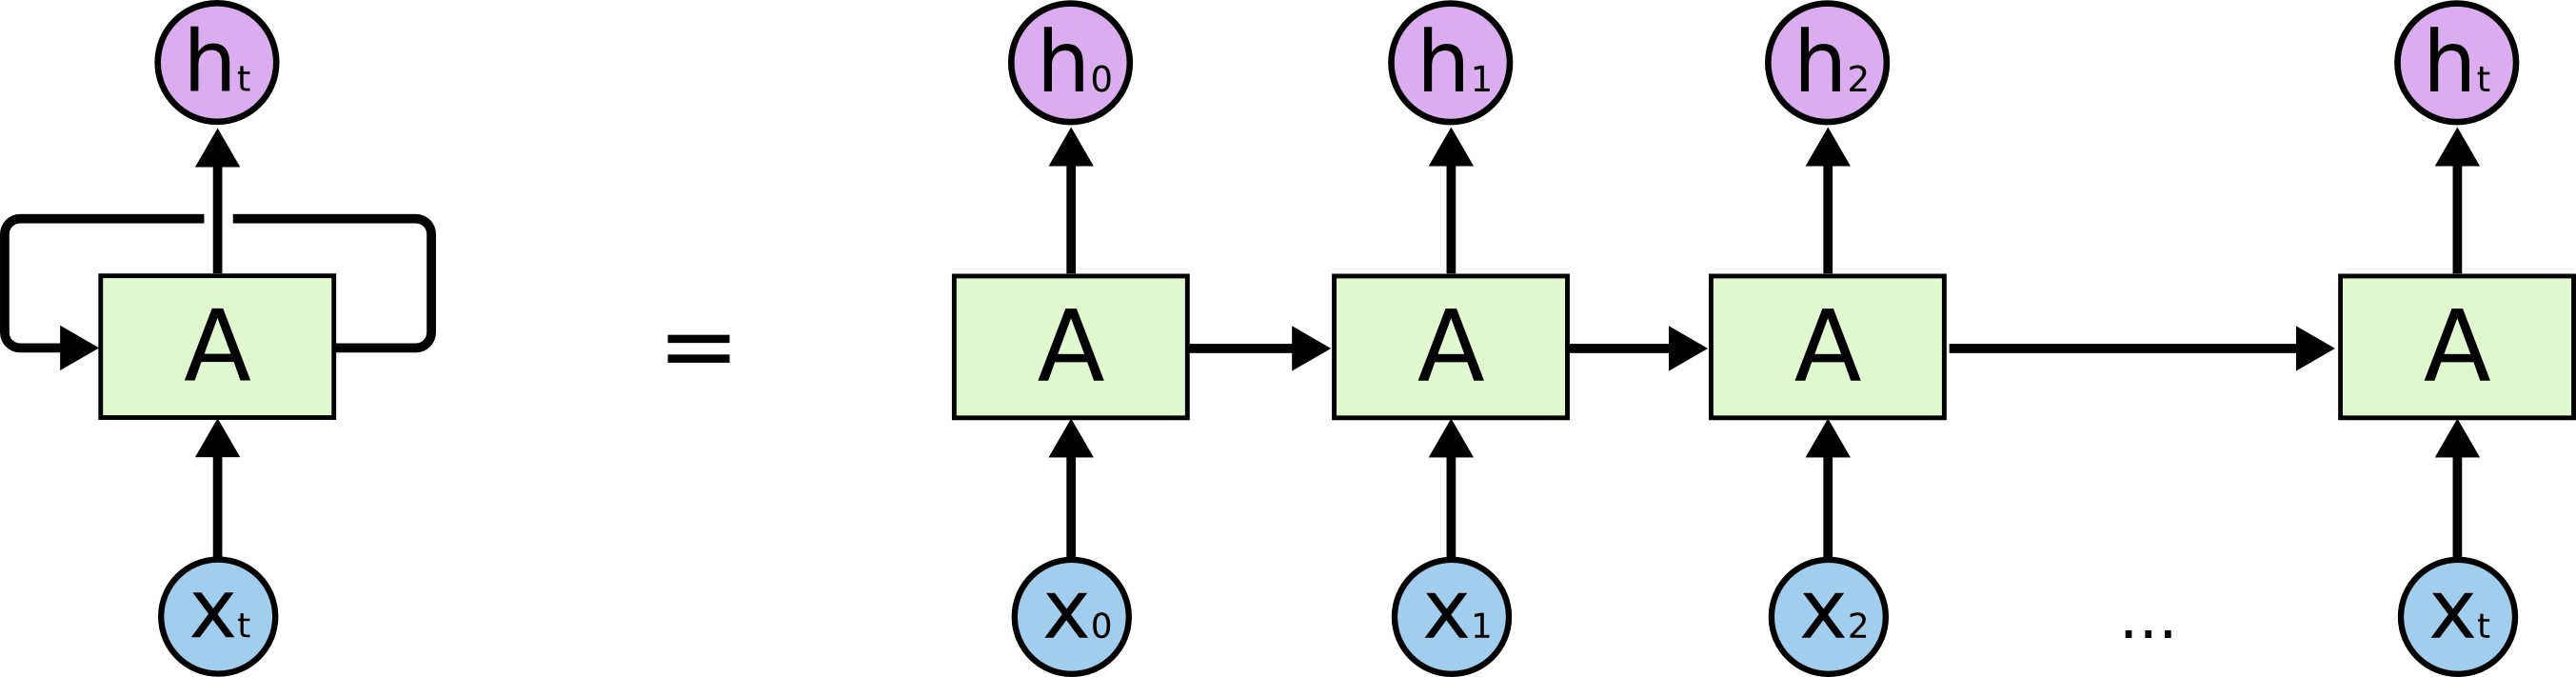
\includegraphics[width=0.8\columnwidth]{Figures/RNN}
    \decoRule
    \caption[An RNN]{A many inputs to many outputs diagram of an RNN (\cite{oinkina})}
    \label{fig:RNN}
\end{figure}

\subsection{Long Short Term Memory}

The Long Short Term Memory model or LSTM was proposed in \citebracks{LSTMs} in order to overcome the gradient problems related to RNNs and thus allow for faster training on long sequences.
They are also capable of learning longer dependencies due to their internal memory. An LSTM cell has three gates: input, forget, and output.
The state of these gates determines whether the cell allows new input, forgets old information, and affects the output at the current time step.
At time step t, the states of the gates are given by:
\begin{equation}
    i_t=\sigma(w_i[h_{t-1},x_t]+b_i)
\end{equation}
\begin{equation}
    f_t=\sigma(w_f[h_{t-1},x_t]+b_f)
\end{equation}
\begin{equation}
    o_t=\sigma(w_o[h_{t-1},x_t]+b_o)
\end{equation}
where $i_t$, $f_t$ and $o_t$ denote the input, forget, and output gates state respectively, $h_{t-1}$ is the output at the previous time step.
$w$ and $b$ represent weights and biases of each gate, $x_t$ is the input to the LSTM cell, and $\sigma (.)$ is the sigmoid function applied elementwise.
The current output of the cell is computed by:
\begin{equation}
    h_t=o_t \circ tanh(c_t)
\end{equation}
\begin{equation}
    c_t = f_t \circ c_{t-1}+i_t \circ \overset{\sim}{c}_t
\end{equation}
\begin{equation}
    \overset{\sim}{c}_t = tanh(w_c[h_t,x_t]+b_c)
\end{equation}

\begin{figure}
    \centering
    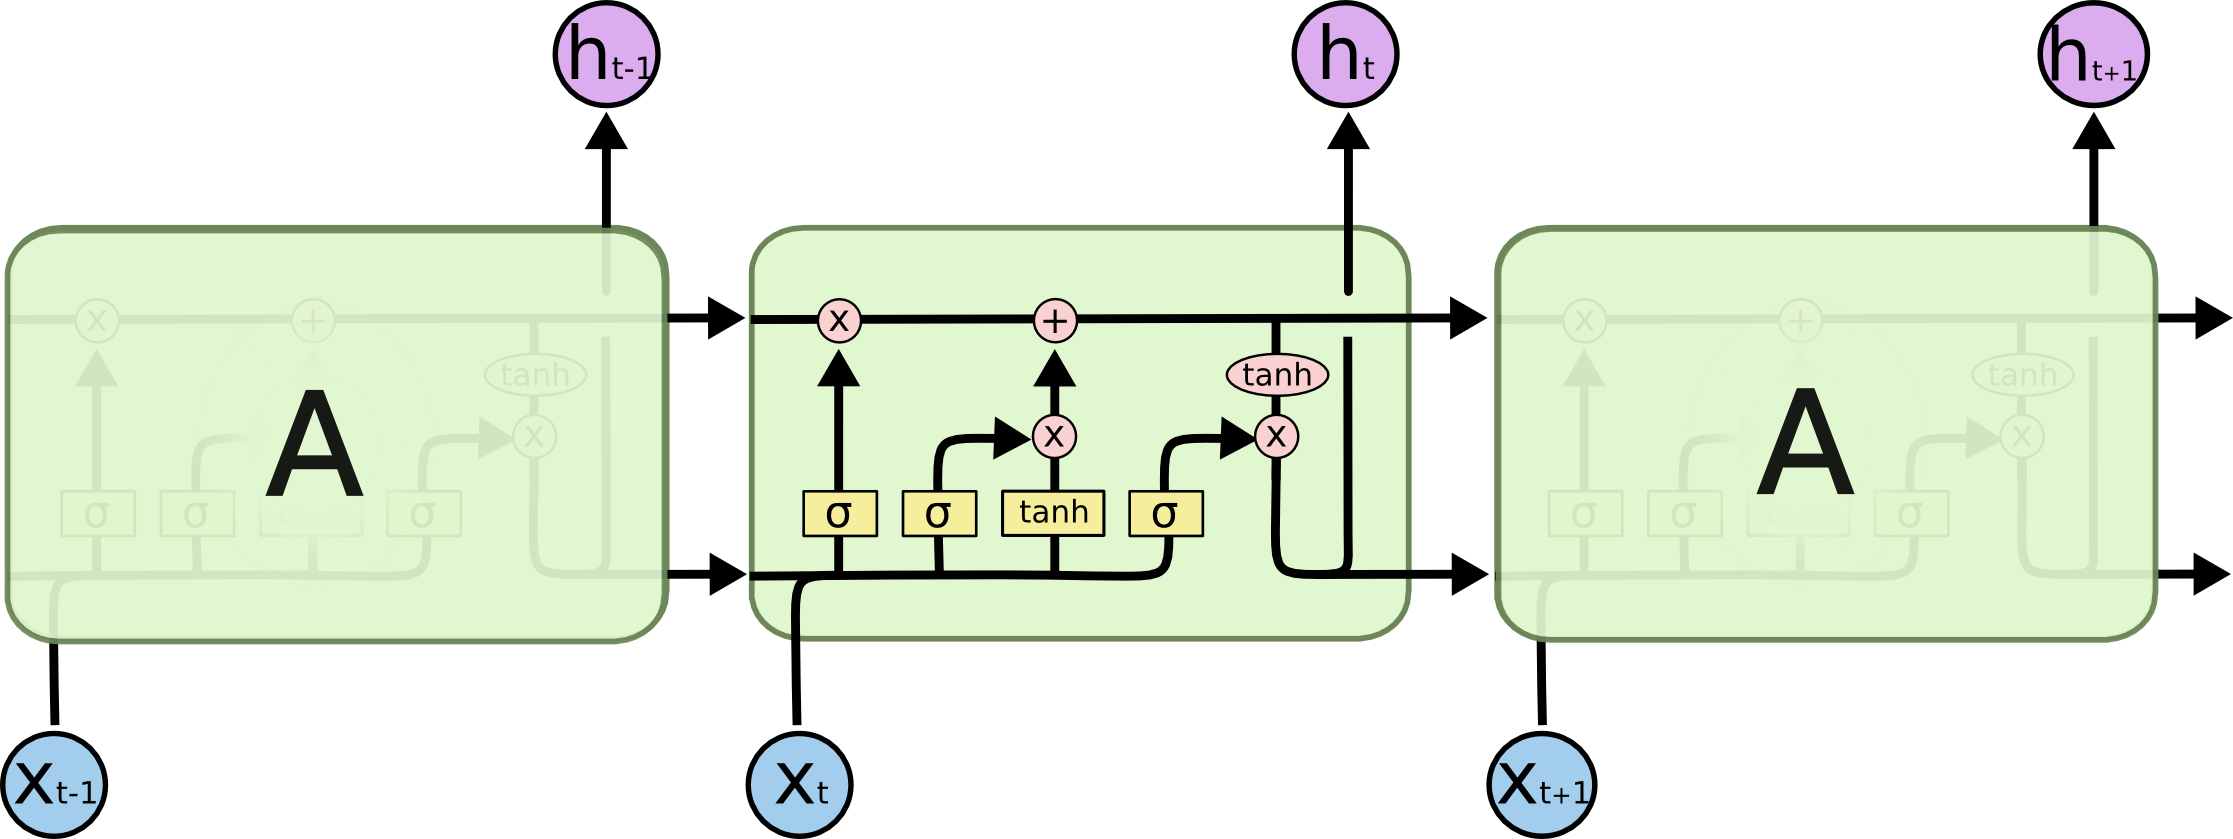
\includegraphics[width=0.8\columnwidth]{Figures/LSTM}
    \decoRule
    \caption{The repeating module in an LSTM (\cite{oinkina})}
    \label{fig:LSTM}
\end{figure}

\subsubsection{Implementations in literature}

\paragraph{Chord Generation from Symbolic Melody - 6} This was the main model under scrutiny in \citebracks{BLSTM} mentioned above in \cref{subsec:HMM} and \cref{subsec:DNN-HMMs}.
They built a bidirectional LSTM with two hidden layers and used a hyperbolic tangent activation function. The softmax function is applied to the output in order to represent the probability that each of the 24 chords is played.
The same dataset as the HMM and DNN-HMM was used and an accuracy of $0.5055$, $0.5032$, $0.4923$, and $0.4990$  was obtained on the 4, 8, 12 and 16 bars respectively. This results in an average accuracy of $0.5000$.
On the user subjective test the LSTM achieved a score of $3.55$.

\paragraph{Automatic Melody Harmonization - 7} A particularly interesting model heavily relying on LSTMs surrounded by a reinforcement learning framework was proposed in \citebracks{ReinforcementLearning}.
They simultaneously trained a Structured Representation Module responsible for learning note-level, phrase-level and segment level representations, a Segmentation Module acting as a reinforcement learning agent to decide whether the current note is the boundary of a phrase or segment and a Harmonisation Module responsible for generating chords for each segment.
They used the Hooktheory Lead Sheet Dataset with 10,000 songs, no number of measures was given but with the difference in model architecture so drastic a comparison on this metric would be inappropriate anyway.
They achieved an accuracy of $0.3742$ and compared that to an SVM, CNN, LSTM and BLSTM with blocked Gibbs sampling which achieved an accuracy of $0.2516$, $0.2664$, $0.2802$, $0.2933$ respectively.
% The inclusion of variable numbers of chords in each measure greatly expands the possibilities with music composition

\subsection{Transformers}
\label{sec:ModelTransformers}
\subsubsection{Explanation and Applicability}

Transformers have been a revolutionary development in the field of NLP, first proposed by \citebracks{Transformers} they have become very widely used and regularly produce state-of-the-art performance.
Transformers utilise the encoder decoder model (\cite{EncoderDecoder}) for sequence to sequence translation.
They also heavily use attention, which is a mechanism for weighting the importance of different elements of a sequence of data.
Specifically, they propose the Scaled dot-product attention shown in \cref{eq:Attention}
\begin{equation}
    \text{Attention}(Q,K,V) = \text{softmax}(\frac{QK^T}{\sqrt{d_k}})V
    \label{eq:Attention}
\end{equation}
where $Q$, $K$ and $V$ represent the queries, keys and values respectively and $d_k$ is the dimension of queries and keys.

\begin{figure}
    \centering
    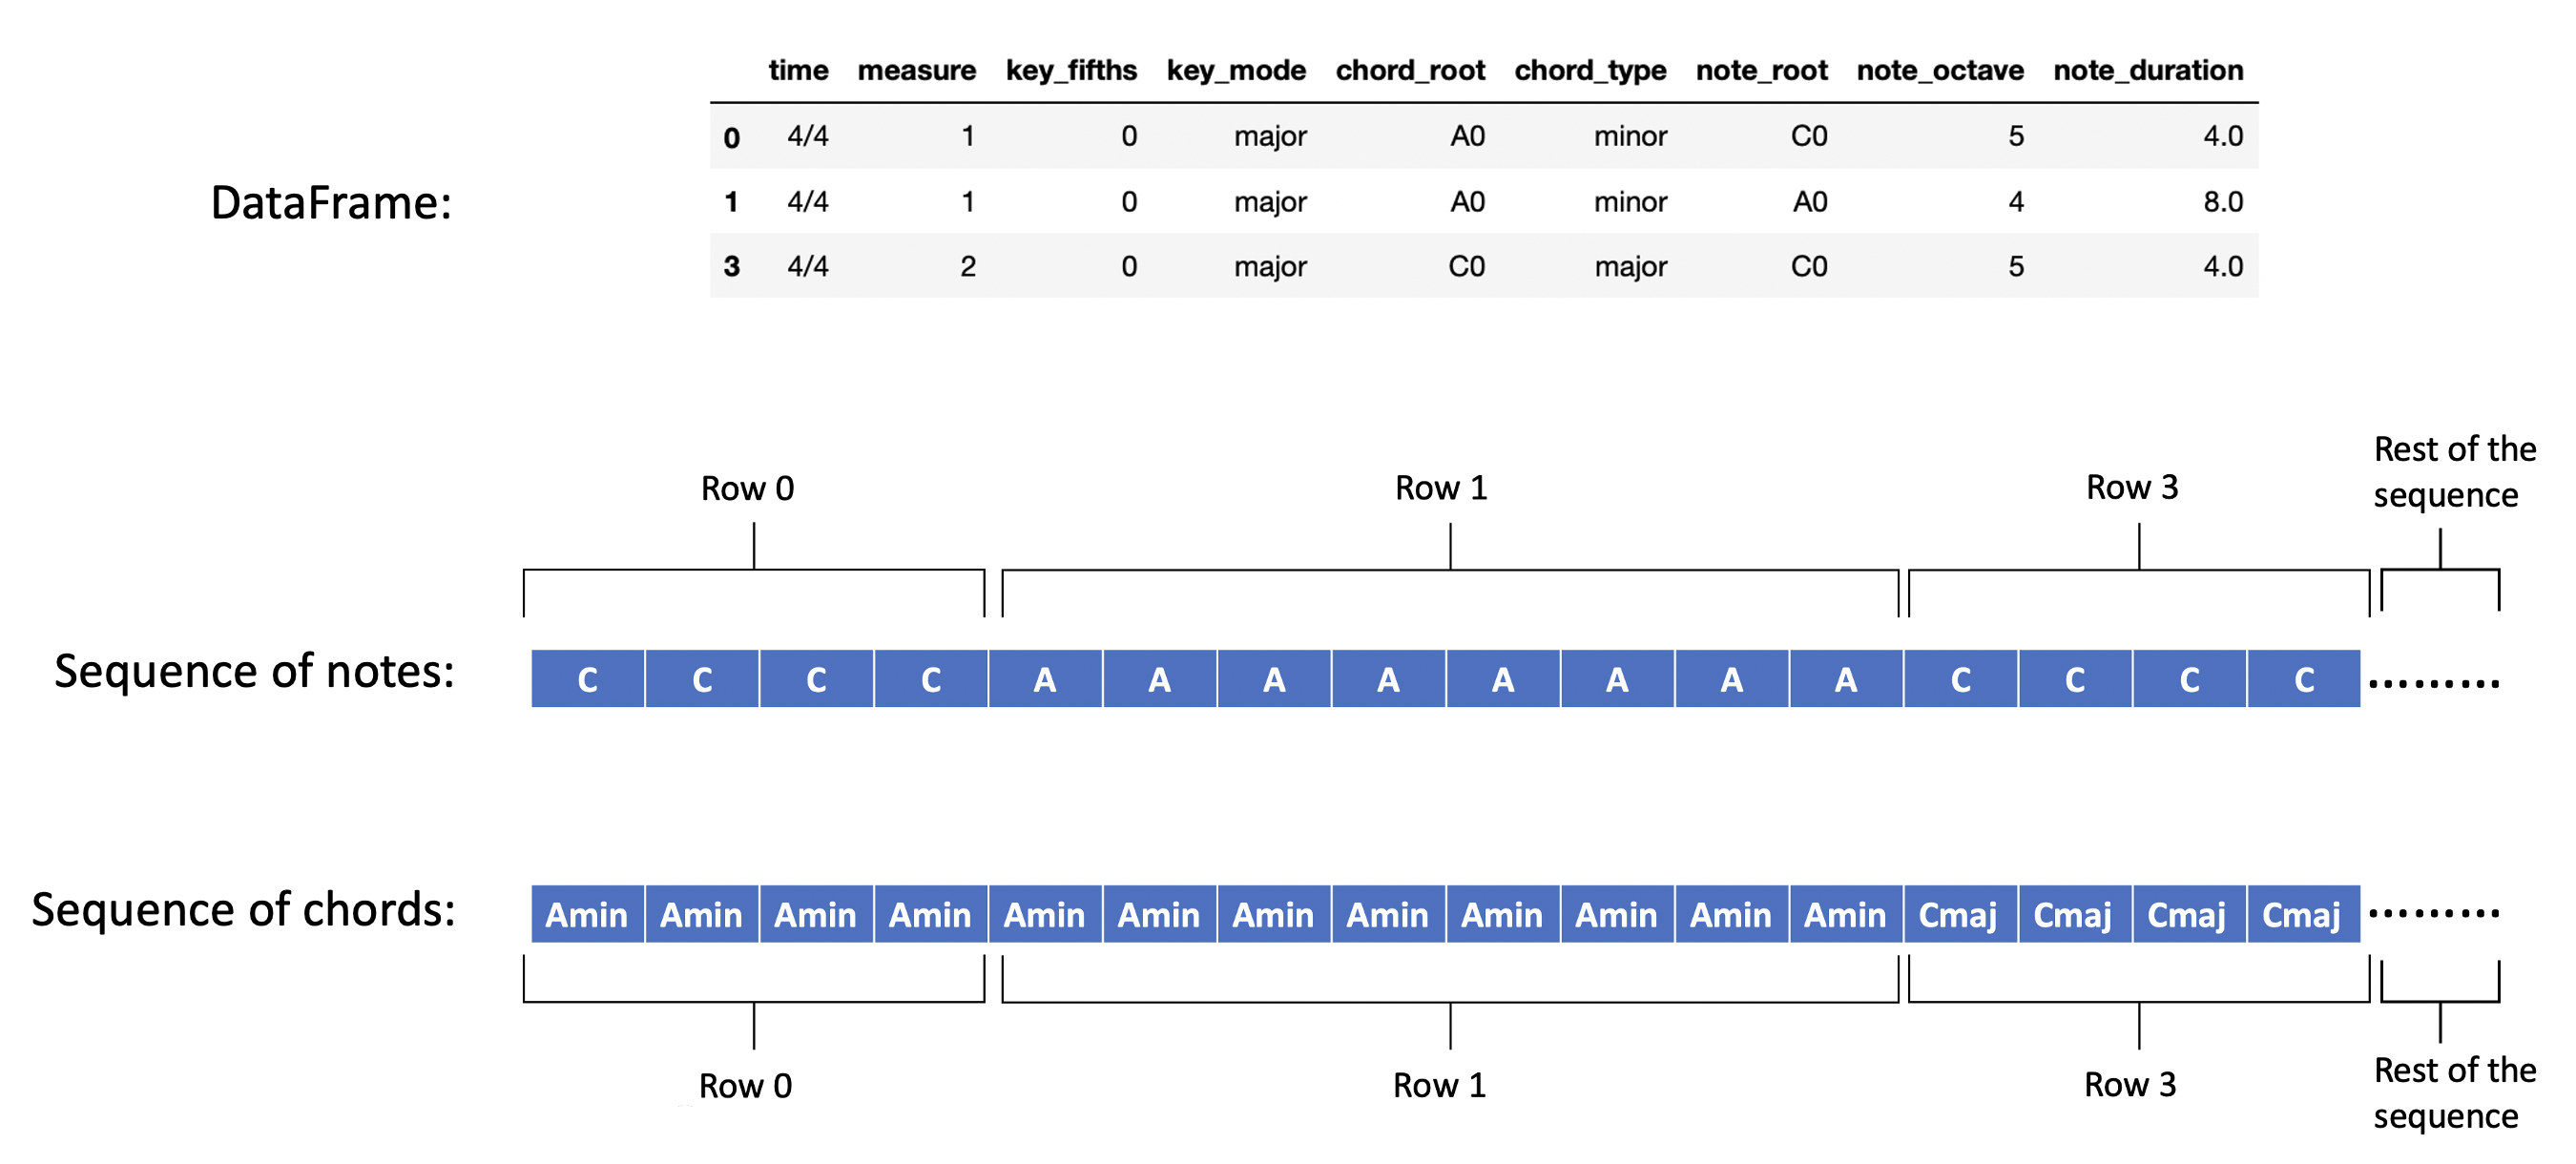
\includegraphics[width=0.6\columnwidth]{Figures/Transformer}
    \decoRule
    \caption{The architecture of a transformer (\cite{Transformers})}
    \label{fig:Transformer}
\end{figure}

The structure of a transformer is shown in \cref{fig:Transformer}.
The masked multi-head attention block is particularly useful for our use case as it allows for the pre specification of output chords.
Therefore, if a user were to particularly like a certain chord or set of chords it would be possible to lock those in place and generate others around it.

\subsubsection{Possible Implementation}
As, to our knowledge, no implementations of a transformer exist to solve this problem, we now outline how this could be achieved.
Transformers require a symbol picked from a finite set. 
In our case these input symbols would correspond to the note played on each submeasure.
This results in the input data format discussed in \cref{Transformer format for training}.
The set of output symbols would then consist of the set of possible chords and there would be an output of one chord per submeasure resulting in the corresponding chord data format.
The structure of the transformer can be that used in \citebracks{Transformers}.
In order to train the model the Adam optimiser (\cite{Adam}) can be used and dropout can be used for regularisation.
Given its success in natural language processing we hypothesise that results from a transformer on this problem would be promising.

\subsection{Summary of Models}

From this evaluation of models and the summary in \cref{tab:modelsummary} we see that the GAN performed particularly well with an accuracy of 0.678.
However, while it is non-deterministic, a GAN  with vanilla neural networks as its generator and discriminator does not take into account the relationship of the chords with the melody at different points in time.
Therefore, in order to use a GAN within our requirements some adjustments are necessary.
The LSTM is a model which is temporally sensitive and which performed well compared to most other models under evaluation.
The LSTM used simply as an input output model is deterministic and thus would not, in the evaluated format, meet our requirements.
It is possible to create a non-deterministic LSTM using the encoder-decoder model mentioned in \cref{sec:ModelTransformers} with decoding strategies designed such that the output is chosen randomly, weighted by the predicted probability that that chord is played.
Another option is to combine the high quality non-deterministic chord generation performance of the GAN with the temporally sensitive LSTM.
How one could go about this is detailed in the next section.

\begin{table}
    \caption{A summary of the models and their performance in evaluation}
    \label{tab:modelsummary}
    \centering
    \begin{tabular}{c c c c c c}
    \toprule
    \tabhead{Model} & & \tabhead{Num Measures} & \tabhead{Accuracy} & \tabhead{Sentiment} \\
    \midrule
    HMMs & 1 & & & 1.8/5 preferred \\
    & 2 & 72,418 & 0.4041 & 2.31/5 \\
    & 3 & 813 & 0.4844 & \\
    \midrule
    DNN-HMMs & 4 & 72,418 & 0.4487 & 2.48/5 \\
    \midrule
     GANs & 5 & & 0.687 & \\
    \midrule
    LSTMs & 6 & 72,418 & 0.500 & 3.55/5 \\
    & 7 & 10,000 songs & 0.2802 & \\
    \bottomrule \\
\end{tabular}
\end{table}

\section{Our Model}
\label{Our Model}
We propose the use of a conditional GAN to learn the association between melodies and chords.
It is well demonstrated that a GAN is capable of generating high quality imitations of real data and as a non-deterministic model it fits the criterial outlined in \cref{sec:MVPRequirements}.
The Discriminator consists of a number of LSTM layers followed by a linear output layer.
The Generator consists of a linear layer followed by a number of LSTM layers and then by another linear layer.
% The Binary Cross Entropy loss is used to determine the Discriminator loss for each example. This is averaged across every measure and then between real and generated examples
\subsection{Components}

\paragraph{Generator}
In essence the Generator functions as a non-deterministic translator, from a sequence of melody vectors to a sequence of chord vectors, and thus models from the NLP space would function appropriately.
Since the LSTM, a common model used in NLP, performed best in \cref{sec:Evaluation} and is strongly affected by the temporal relationship between inputs, we chose to use it in our Generator.
It takes as input, a tensor of dimensions $(b,n,12+l)$ where $b$ is the batch size, $n$ is the number of measures in the song and $l$ is the length of the noise vector.
Each batch is treated independently and identically, so we will proceed discussing the treatment of the 2nd and 3rd dimensions, and it can be assumed this is repeated $b$ times.
Thus, we effectively input a tensor of dimensions $(n,12+l)$ into the first layer of the Generator.
We input the vectors into a linear layer followed by a ReLU activation function. 
These are followed by $k$ layers of bidirectional LSTMs.
In the first layer each pair of LSTM cells, one for the forward direction and one for the reverse direction, takes an input vector of length 37, representing a melody vector concatenated with a chord vector and outputs a vector of length $h$ corresponding to the size of the hidden layers.
The LSTM cells in the subsequent $k-1$ layers have both input and output sizes of $h$.
The output of the final LSTM layer is fed into a final linear layer which takes input of size $h$ and outputs a vector of length 25, representing the chords.
This is then passed through a softmax layer which gives the probability that each chord is played at each point in time.

\begin{figure}
    \centering
    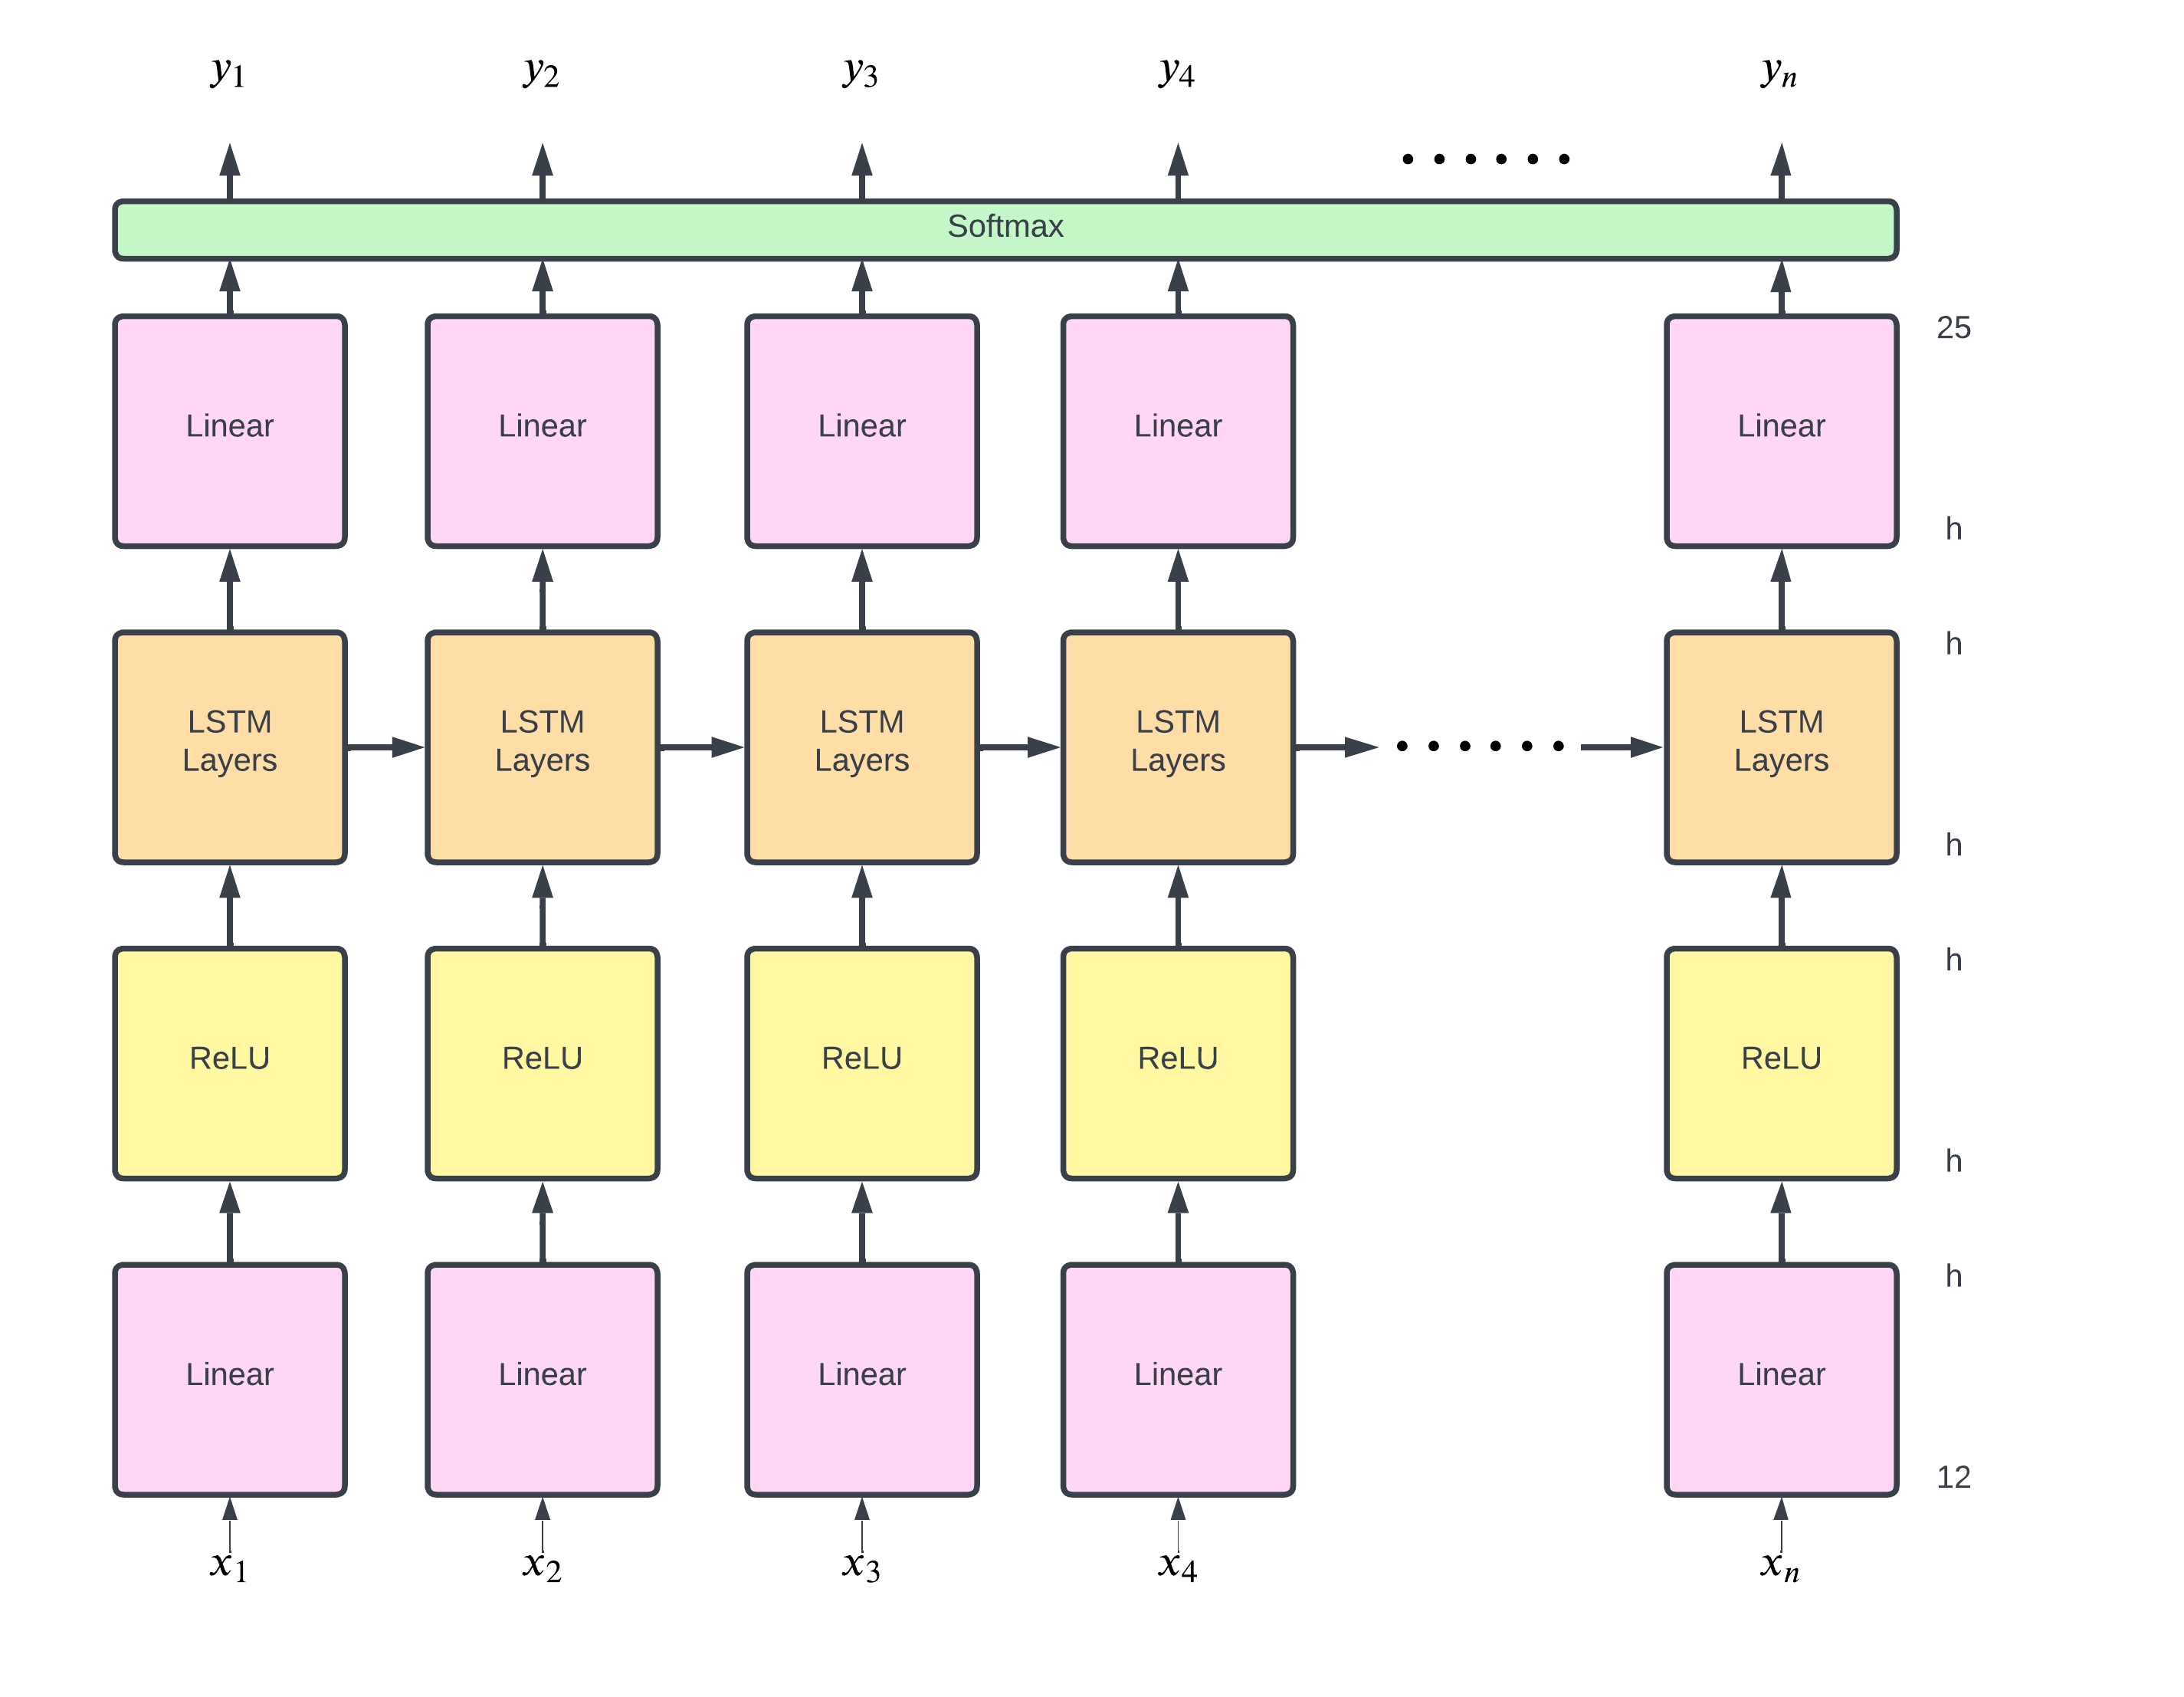
\includegraphics[width=0.8\columnwidth]{Figures/Generator}
    \decoRule
    \caption{The architecture of our Generator}
    \label{fig:Generator}
\end{figure}

\paragraph{Discriminator}
The Discriminator is a binary sequence classifier, outputting whether the input was real or generated.
It takes as input a tensor of dimensions $(b,n,37)$ where $b$ is the batch size and $n$ is the number of measures in the song.
Each batch is treated independently and identically, so we will proceed discussing the treatment of the 2nd and 3rd dimensions, and it can be assumed this is repeated $b$ times.
Thus, we effectively input a tensor of dimensions $(n,37)$ into the first layer of the Discriminator.
The first $k$ layers of the Discriminator are bidirectional LSTMs. 
These function much like they do in the Generator.
The fully connected layer takes and input of size $2 \times n \times h$ and outputs a vector of size 1.
The output is passed through a sigmoid activation function thus converting it to represent the probability that the input melody sequence, chord sequence pair was from a real song.

\begin{figure}
    \centering
    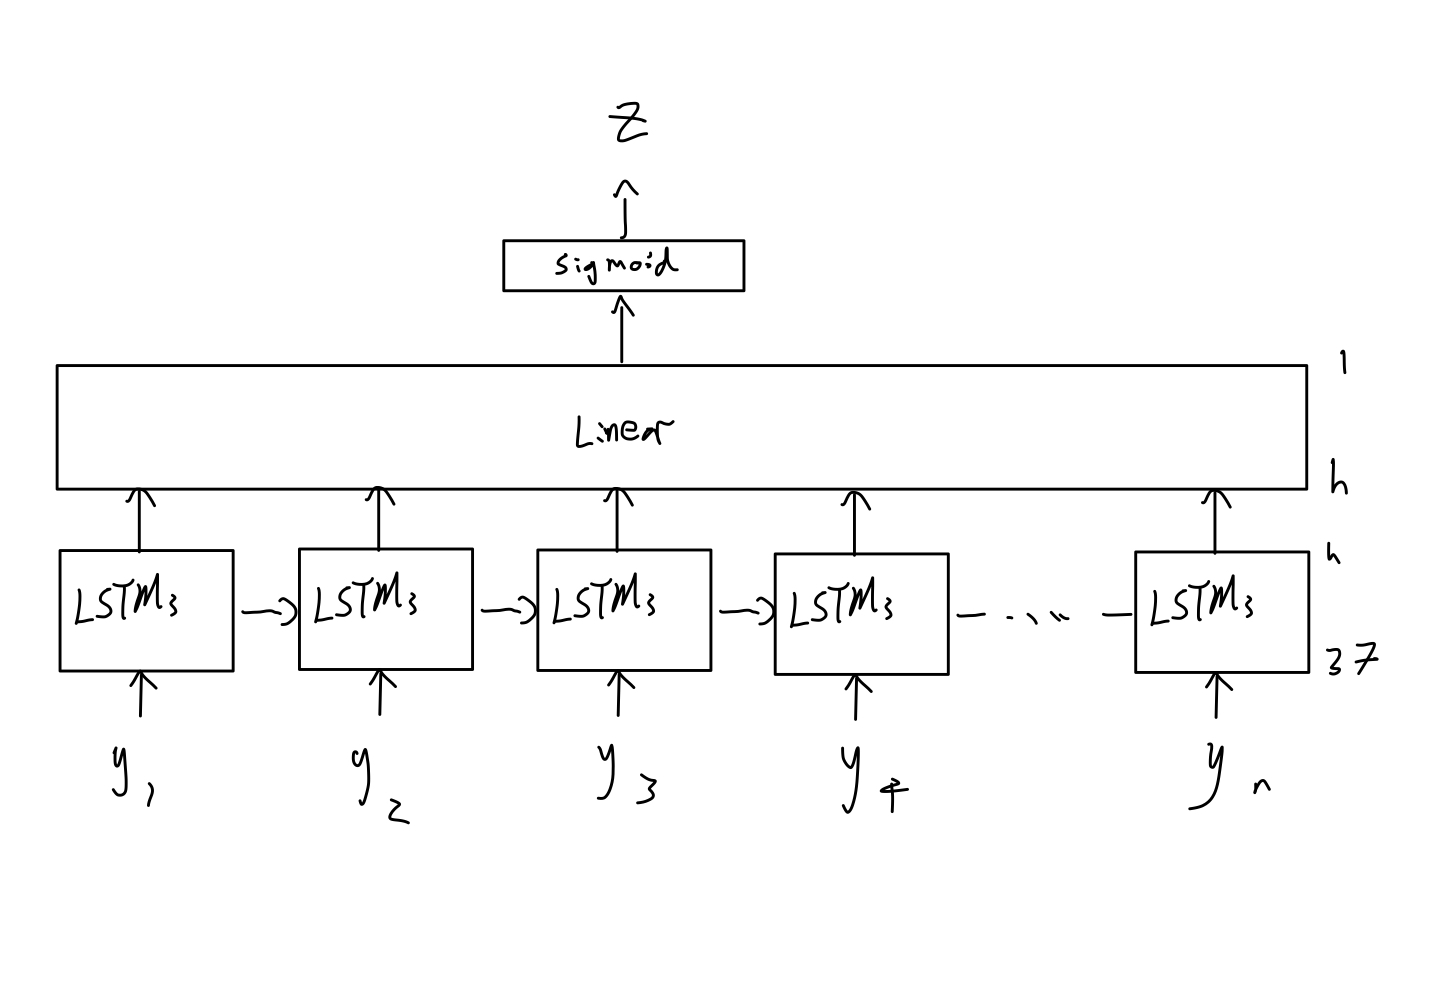
\includegraphics[width=0.8\columnwidth]{Figures/Discriminator}
    \decoRule
    \caption{The architecture of our Discriminator}
    \label{fig:Discriminator}
\end{figure}


\subsection{Model Functionality}

As proof of concept for the design, we developed a command line based interface for the model so that it was easy to train, vary parameters, and test. 
In production the user would be able to utilise a subset of this interface, such as the option to generate accompaniment and have it played back, through a graphical user interface detailed in \cref{Chapter2}.
The options available in the interface are shown in \cref{tab:parameters}

\begin{table}
    \caption{The parameters of the command line interface for the model}
    \label{tab:parameters}
    \centering
    \begin{tabular}{l l l p{0.5\linewidth}}
    \toprule
    \tabhead{Parameter} & \tabhead{Options} & \tabhead{Default} & \tabhead{Description} \\
    \midrule
    \code{-input\_size} & \code{[input\_size]} & $12$ & The size of the input vector to the discriminator representing the melody  \\
    \code{-output\_size} & \code{[output\_size]} & $25$ & The size of the output vector representing the chord played in each measure \\
    \code{-h\_size} & \code{[h\_size]} & $128$ & The size of the hidden layers in the LSTM layers \\
    \code{-n\_layers} & \code{[n\_layers]} & $2$ & The number of LSTM layers in the generator and discriminator \\
    \code{-noise\_size} & \code{[noise\_size]} & $12$ & The size of the noise vector concatenated with the input vector to the generator \\
    \code{-max\_seqlen} & \code{[max\_seqlen]} & $200$ & The maximum length of song in measures used in training \\
    \code{-src\_data} & \code{[src\_data]} &  & The default path to the training data \\
    \code{-batch\_size} & \code{[batch\_size]} & $10$ & The size of the batches used in the stochastic gradient descent algorithm \\
    \code{-epochs} & \code{[epochs]} & $100$ & The number of epochs used in training \\
    \code{-printevery} & \code{[printevery]} & $10$ & The number of epochs between printing an example during training \\
    \code{-load} & & False & Whether to load a model in or not \\
    \code{-load\_dir} & \code{[load\_dir]} &  & The path to the folder containing pretrained models \\
    \code{-model\_num} & \code{[model\_num]} & $1$ & The number of the model to be loaded in \\
    \code{-save} & & False & Whether to save the model after training \\
    \code{-save\_dir} & \code{[save\_dir]} &  & The path to the save directory \\
    \code{-playback} & & False & Whether to play an example of generated music at the end of training \\
    \bottomrule \\
\end{tabular}
\end{table}
 
\paragraph{DataLoader} 
We created a MusicDataset class inheriting from a PyTorch Dataset to load in the data in an useable form.
Since our model takes a fixed sequence length and not all songs are of equal length we zero-pad all songs so that their length is equal to that of the longest song.
The chords are padded with vectors representing a rest.

\section{Training}

\begin{figure}
    \centering
    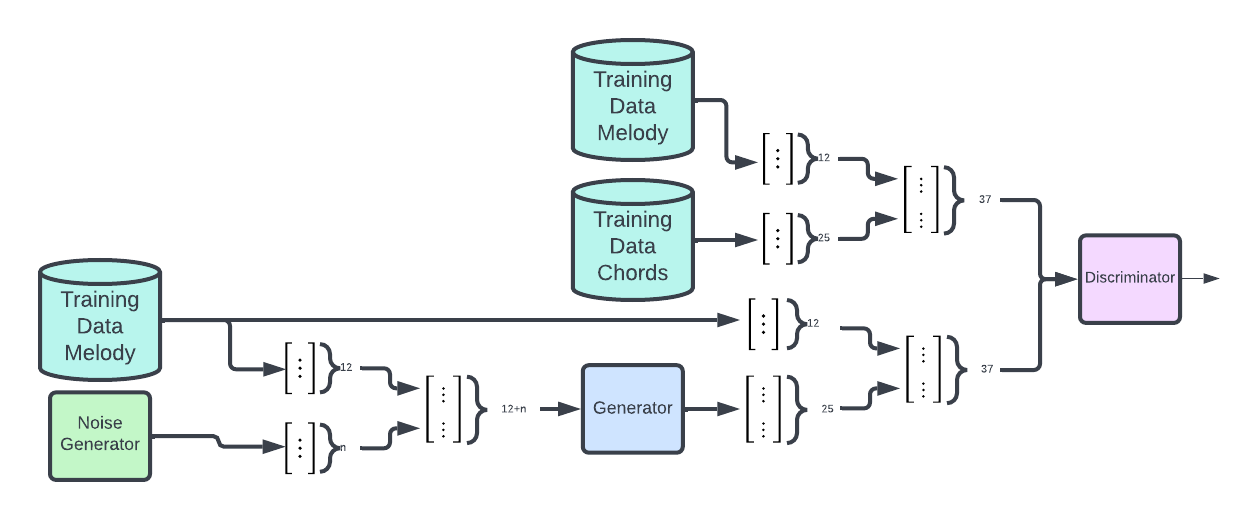
\includegraphics[width=\columnwidth]{Figures/GAN}
    \decoRule
    \caption{The training of the model}
    \label{fig:ModelTraining}
\end{figure}

\paragraph{Loss}
A loss function is used to gain a measure of how different the output of the model is from the desired output.
For best results, a loss function is often coupled with the activation function of the linear layers.
An example of this coupling is the sigmoid activation function and the binary cross entropy. %\textbf{EXPAND ON THIS}
As we are using a GAN we use the binary cross entropy or BCE as our loss function for the discriminator since we are dealing with the binary problem, is the input real or generated?
The discriminator loss is averaged across its performance between real and generated examples.
For the generator we use the complement of the Discriminator loss on generated examples.
The BCE loss can be calculated as in \cref{eq:BCELoss}.
\begin{equation}
    \label{eq:BCELoss}
    \frac{1}{N} \sum_{i=1}^N log(p(y_i))
\end{equation}
    which for the discriminator takes the form
\begin{equation}
    \frac{1}{N} \sum_{i=1}^N log(D(conc(x_i,z_i))) + log(1-D(conc(G(z_i),z_i)))
\end{equation}
    where $x_i$ are the real examples, $z_i$ are the melodies and the $conc$ function concatenates the two vector arguments.
    The loss is the sum of the loss of the discriminator on real data and generated data.
    The generator loss is
\begin{equation}
    -\frac{1}{N} \sum_{i=1}^N log(1-D(conc(G(z_i),z_i)))
\end{equation}
    which results in trying to maximise the loss of the discriminator on generated data.
    This is equivalent to finding the discriminator loss on generated data when labelled as real which is the method we use in our implementation.

    
\paragraph{Optimiser}
An optimiser is used to determine the changes of model parameters that need to be made to minimise the loss of a model.
Optimisers usually involve the use of the gradient of the model with respect to different parameters.
The standard tool to find the gradients is the backpropagation algorithm 
which is very easy to use with PyTorch.
Gradient descent is an example of a basic optimiser.
We used the Adam optimiser (\cite{Adam}) which is recommended in the Stanford \href{https://cs231n.github.io/}{CS231n: Convolutional Neural Networks for Visual Recognition}\footnote{https://cs231n.github.io/} as the default optimiser.




\subsection{Avoiding Overfitting}
A common problem in machine learning is overfitting. This is where a dataset is modelled to such a precision that noise in the dataset is learned.
This results in the model missing the overarching distribution of the data and thus cannot extend to other data.
There is a number of techniques to avoid overfitting.
Dropout is where neurons are ignored with a given probability on any given pass. 
This is equivalent to training a number of different neural networks which all overfit in different ways thus on average the overfitting will cancel out.
Another technique to reducing overfitting specific to GANs is to use the Wasserstein loss function (\cite{Wasserstein}) rather than the binary cross entropy. 
It uses the difference of the output from the discriminator on real and generated data as the discriminator loss, and uses the output of the discriminator on generated data as the generator loss.
This means that gradients do not vanish as fast, however, the output of the discriminator no longer represents the probability of the input being true.
Another technique is reducing number of LSTM layers. 
This reduces the complexity of the model and thus makes it harder to train it to overfit onto noise.

% \subsection{Issues}
% Training is conducted in batches of a given size.
% It is unlikely that the size of the dataset is divisible by the batch size, so the final batch is likely to be shorter than the others.
% This initially caused problems, however, we were able to set the dimensions of relevant objects, such as the input noise to the generator, to be relative to the current batch size rather than the usual batch size thus solving the problem.
% Softmaxing of outputs of generator
% Device management

\subsection{Testing}
The Model can be tested using the test set as this will reveal any overfitting from training. 
We can evaluate the model as stated in \cref{sec:Evaluation} using the accuracy of the model across the test set.
Another way we can evaluate the model to get a better sense of where and how the model is going wrong is by using a confusion matrix.
We enumerate the generated chords and the true chords. 
For each melody we add one to the element in the (generated chord, true chord) coordinate. 
Thus, an ideal output would be a diagonal matrix such that the generated chord was always the same as the true chord, however, this would also suggest overfitting.
An example of a confusion matrix is shown in \cref{fig:confusion_ideal}
Another form of testing that could be performed is a subjective study like those in \citebracks{MySong} and \citebracks{BLSTM}.
Ideally the studies would be carried out as similarly as possible to the others so that the models they are testing can be reliably compared.


\section{Results}
Unfortunately due to implementation difficulties followed by the sudden death of the machine we were using to train the model we were unable to obtain any valid results.
While the machine was still running we conducted some preliminary training attempts where convergence of the GAN illuded us.
The discriminator quickly learned to distinguish between the real and generated chords and the generator was never able to improve sufficiently to counter this.
The loss of the models can be seen in \cref{fig:ModelLoss}.
It was noticed that the generator converged to predict the same chord on every output. 
This is likely due to a combination of overfitting of the linear output layer in the generator and the vanishing of gradients as the discriminator loss approached zero.
A confusion matrix of these results can be seen in \cref{fig:confusion_real}. The code for this project can be found \href{https://github.com/edsgunn/TerrenceInABox}{here}\footnote{https://github.com/edsgunn/TerrenceInABox}.


\begin{figure}
    \centering
    \begin{subfigure}{0.3\columnwidth}
        \centering
        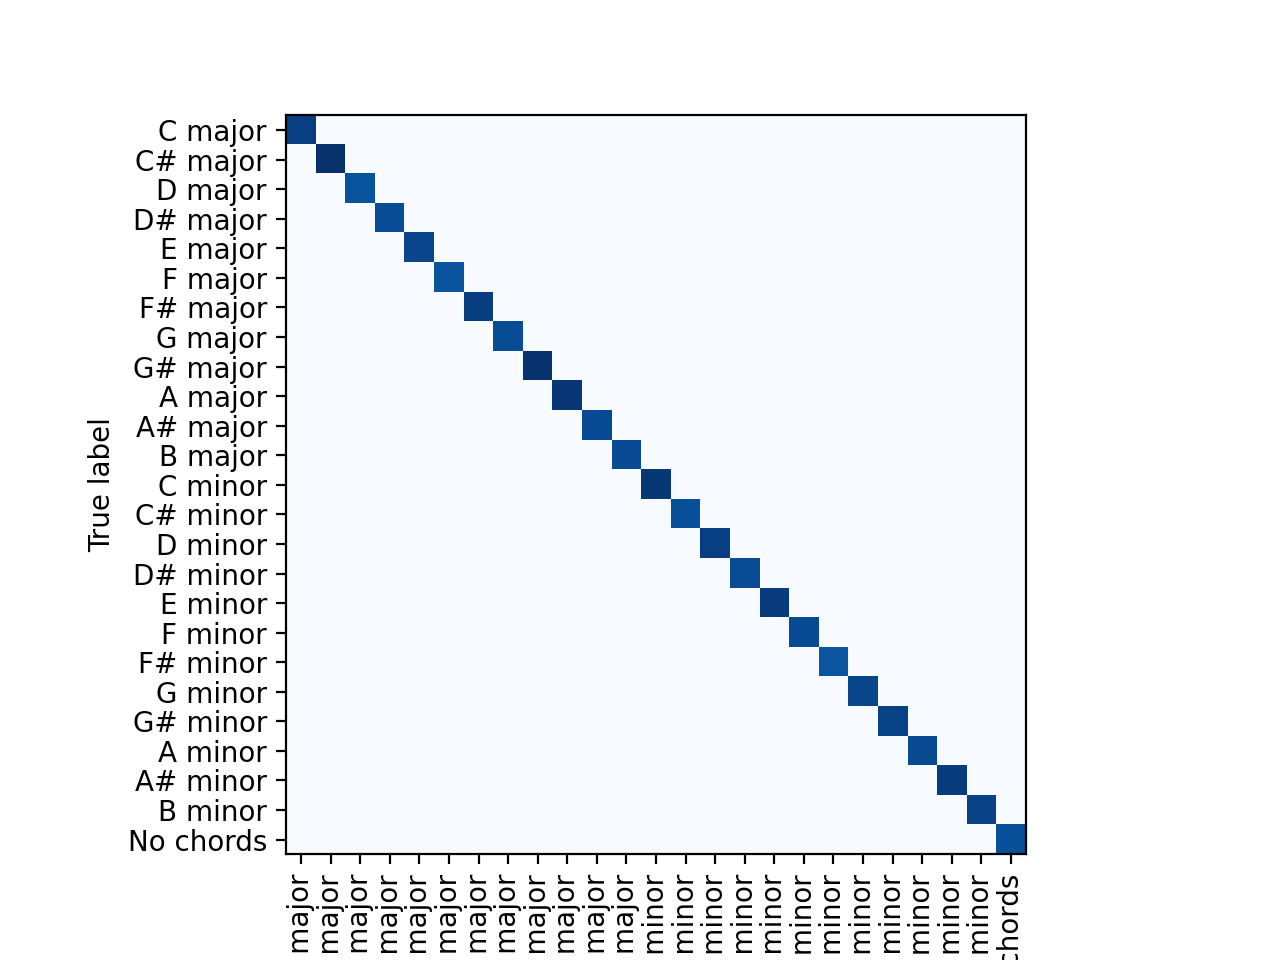
\includegraphics[width=\columnwidth]{Figures/confusion_ideal}
        \decoRule
        \caption{An ideal confusion matrix}
        \label{fig:confusion_ideal}
    \end{subfigure}
    \hfill
    \begin{subfigure}{0.3\columnwidth}
        \centering
        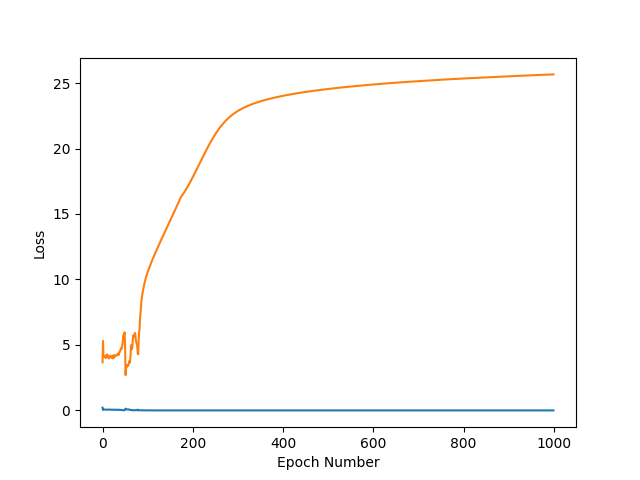
\includegraphics[width=\columnwidth]{Figures/ModelLoss}
        \decoRule
        \caption{The loss of the Generator and Discriminator, blue and orange respectively}
        \label{fig:ModelLoss}
    \end{subfigure}
    \hfill
    \begin{subfigure}{0.3\columnwidth}
        \centering
        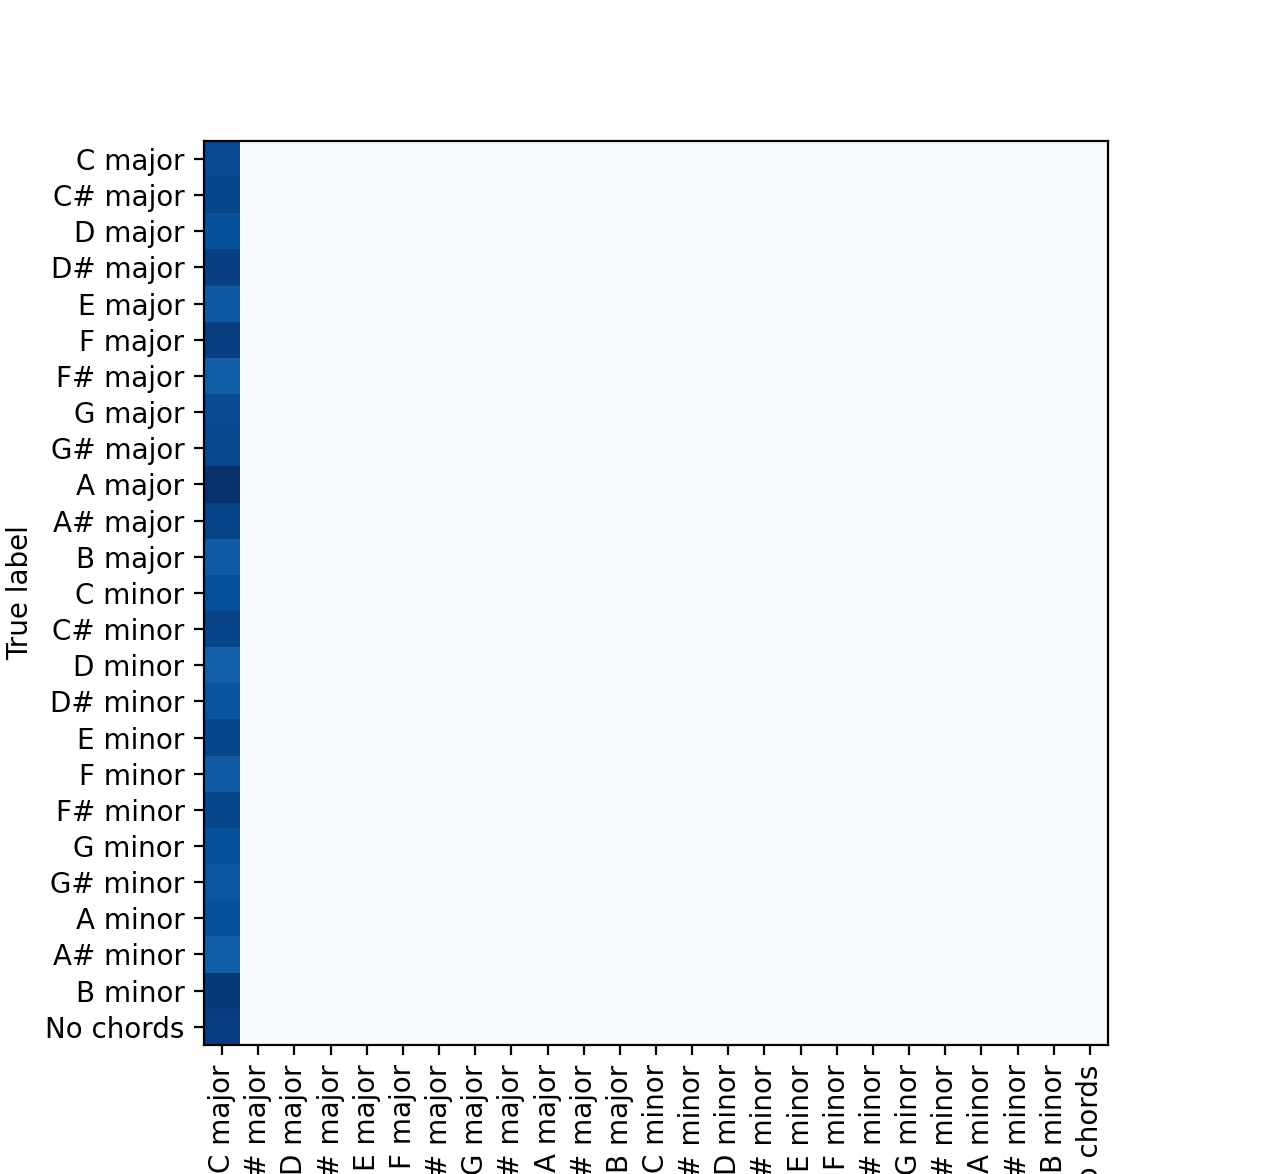
\includegraphics[width=\columnwidth]{Figures/confusion_real}
        \decoRule
        \caption{A confusion matrix of the chords outputted from the model}
        \label{fig:confusion_real}
    \end{subfigure}
    \caption{Quantitative measures of the quality of our model vs the ideal case}
\end{figure}
\section{Summary}

We have discussed the requirements for the model and how we set the MVP requirements to create a system that can generate reasonable accompanying chords for a melody.
The final requirements reached were: black box interface, good sounding chords, designed for sequential data, conditional and one chord per measure.
We developed criteria for evaluation of models expected to satisfy these requirements.
These criteria were: number of measures in training dataset, accuracy in testing, human sentiment towards generated chords and extra functionality.  
We applied these to a number of models implemented in other papers and found a combination of the models to be a promising solution. 
The use of an LSTMGAN as a solution to this problem was proposed hypothesising that the combination of the quality providing GAN and the sequential LSTM would produce high quality outputs.
This model design was detailed with a breakdown of the function and structure of the generator and discriminator as well as the training process.
We implemented, trained and tested the model for preliminary investigation, however, our results were unsatisfactory due to system difficulties.
 


% % Chapter 1

\chapter{Chapter Title Here} % Main chapter title

\label{ChapterX} % For referencing the chapter elsewhere, use \ref{Chapter1} 

%----------------------------------------------------------------------------------------

% Define some commands to keep the formatting separated from the content 
\newcommand{\keyword}[1]{\textbf{#1}}
\newcommand{\tabhead}[1]{\textbf{#1}}
\newcommand{\code}[1]{\texttt{#1}}
\newcommand{\file}[1]{\texttt{\bfseries#1}}
\newcommand{\option}[1]{\texttt{\itshape#1}}

%----------------------------------------------------------------------------------------

\section{Welcome and Thank You}
Welcome to this \LaTeX{} Thesis Template, a beautiful and easy to use template for writing a thesis using the \LaTeX{} typesetting system.

If you are writing a thesis (or will be in the future) and its subject is technical or mathematical (though it doesn't have to be), then creating it in \LaTeX{} is highly recommended as a way to make sure you can just get down to the essential writing without having to worry over formatting or wasting time arguing with your word processor.

\LaTeX{} is easily able to professionally typeset documents that run to hundreds or thousands of pages long. With simple mark-up commands, it automatically sets out the table of contents, margins, page headers and footers and keeps the formatting consistent and beautiful. One of its main strengths is the way it can easily typeset mathematics, even \emph{heavy} mathematics. Even if those equations are the most horribly twisted and most difficult mathematical problems that can only be solved on a super-computer, you can at least count on \LaTeX{} to make them look stunning.

%----------------------------------------------------------------------------------------

\section{Learning \LaTeX{}}

\LaTeX{} is not a \textsc{wysiwyg} (What You See is What You Get) program, unlike word processors such as Microsoft Word or Apple's Pages. Instead, a document written for \LaTeX{} is actually a simple, plain text file that contains \emph{no formatting}. You tell \LaTeX{} how you want the formatting in the finished document by writing in simple commands amongst the text, for example, if I want to use \emph{italic text for emphasis}, I write the \verb|\emph{text}| command and put the text I want in italics in between the curly braces. This means that \LaTeX{} is a \enquote{mark-up} language, very much like HTML.

\subsection{A (not so short) Introduction to \LaTeX{}}

If you are new to \LaTeX{}, there is a very good eBook -- freely available online as a PDF file -- called, \enquote{The Not So Short Introduction to \LaTeX{}}. The book's title is typically shortened to just \emph{lshort}. You can download the latest version (as it is occasionally updated) from here:
\url{http://www.ctan.org/tex-archive/info/lshort/english/lshort.pdf}

It is also available in several other languages. Find yours from the list on this page: \url{http://www.ctan.org/tex-archive/info/lshort/}

It is recommended to take a little time out to learn how to use \LaTeX{} by creating several, small `test' documents, or having a close look at several templates on:\\ 
\url{http://www.LaTeXTemplates.com}\\ 
Making the effort now means you're not stuck learning the system when what you \emph{really} need to be doing is writing your thesis.

\subsection{A Short Math Guide for \LaTeX{}}

If you are writing a technical or mathematical thesis, then you may want to read the document by the AMS (American Mathematical Society) called, \enquote{A Short Math Guide for \LaTeX{}}. It can be found online here:
\url{http://www.ams.org/tex/amslatex.html}
under the \enquote{Additional Documentation} section towards the bottom of the page.

\subsection{Common \LaTeX{} Math Symbols}
There are a multitude of mathematical symbols available for \LaTeX{} and it would take a great effort to learn the commands for them all. The most common ones you are likely to use are shown on this page:
\url{http://www.sunilpatel.co.uk/latex-type/latex-math-symbols/}

You can use this page as a reference or crib sheet, the symbols are rendered as large, high quality images so you can quickly find the \LaTeX{} command for the symbol you need.

\subsection{\LaTeX{} on a Mac}
 
The \LaTeX{} distribution is available for many systems including Windows, Linux and Mac OS X. The package for OS X is called MacTeX and it contains all the applications you need -- bundled together and pre-customized -- for a fully working \LaTeX{} environment and work flow.
 
MacTeX includes a custom dedicated \LaTeX{} editor called TeXShop for writing your `\file{.tex}' files and BibDesk: a program to manage your references and create your bibliography section just as easily as managing songs and creating playlists in iTunes.

%----------------------------------------------------------------------------------------

\section{Getting Started with this Template}

If you are familiar with \LaTeX{}, then you should explore the directory structure of the template and then proceed to place your own information into the \emph{THESIS INFORMATION} block of the \file{main.tex} file. You can then modify the rest of this file to your unique specifications based on your degree/university. Section \ref{FillingFile} on page \pageref{FillingFile} will help you do this. Make sure you also read section \ref{ThesisConventions} about thesis conventions to get the most out of this template.

If you are new to \LaTeX{} it is recommended that you carry on reading through the rest of the information in this document.

Before you begin using this template you should ensure that its style complies with the thesis style guidelines imposed by your institution. In most cases this template style and layout will be suitable. If it is not, it may only require a small change to bring the template in line with your institution's recommendations. These modifications will need to be done on the \file{MastersDoctoralThesis.cls} file.

\subsection{About this Template}

This \LaTeX{} Thesis Template is originally based and created around a \LaTeX{} style file created by Steve R.\ Gunn from the University of Southampton (UK), department of Electronics and Computer Science. You can find his original thesis style file at his site, here:
\url{http://www.ecs.soton.ac.uk/~srg/softwaretools/document/templates/}

Steve's \file{ecsthesis.cls} was then taken by Sunil Patel who modified it by creating a skeleton framework and folder structure to place the thesis files in. The resulting template can be found on Sunil's site here:
\url{http://www.sunilpatel.co.uk/thesis-template}

Sunil's template was made available through \url{http://www.LaTeXTemplates.com} where it was modified many times based on user requests and questions. Version 2.0 and onwards of this template represents a major modification to Sunil's template and is, in fact, hardly recognisable. The work to make version 2.0 possible was carried out by \href{mailto:vel@latextemplates.com}{Vel} and Johannes Böttcher.

%----------------------------------------------------------------------------------------

\section{What this Template Includes}

\subsection{Folders}

This template comes as a single zip file that expands out to several files and folders. The folder names are mostly self-explanatory:

\keyword{Appendices} -- this is the folder where you put the appendices. Each appendix should go into its own separate \file{.tex} file. An example and template are included in the directory.

\keyword{Chapters} -- this is the folder where you put the thesis chapters. A thesis usually has about six chapters, though there is no hard rule on this. Each chapter should go in its own separate \file{.tex} file and they can be split as:
\begin{itemize}
\item Chapter 1: Introduction to the thesis topic
\item Chapter 2: Background information and theory
\item Chapter 3: (Laboratory) experimental setup
\item Chapter 4: Details of experiment 1
\item Chapter 5: Details of experiment 2
\item Chapter 6: Discussion of the experimental results
\item Chapter 7: Conclusion and future directions
\end{itemize}
This chapter layout is specialised for the experimental sciences, your discipline may be different.

\keyword{Figures} -- this folder contains all figures for the thesis. These are the final images that will go into the thesis document.

\subsection{Files}

Included are also several files, most of them are plain text and you can see their contents in a text editor. After initial compilation, you will see that more auxiliary files are created by \LaTeX{} or BibTeX and which you don't need to delete or worry about:

\keyword{example.bib} -- this is an important file that contains all the bibliographic information and references that you will be citing in the thesis for use with BibTeX. You can write it manually, but there are reference manager programs available that will create and manage it for you. Bibliographies in \LaTeX{} are a large subject and you may need to read about BibTeX before starting with this. Many modern reference managers will allow you to export your references in BibTeX format which greatly eases the amount of work you have to do.

\keyword{MastersDoctoralThesis.cls} -- this is an important file. It is the class file that tells \LaTeX{} how to format the thesis. 

\keyword{main.pdf} -- this is your beautifully typeset thesis (in the PDF file format) created by \LaTeX{}. It is supplied in the PDF with the template and after you compile the template you should get an identical version.

\keyword{main.tex} -- this is an important file. This is the file that you tell \LaTeX{} to compile to produce your thesis as a PDF file. It contains the framework and constructs that tell \LaTeX{} how to layout the thesis. It is heavily commented so you can read exactly what each line of code does and why it is there. After you put your own information into the \emph{THESIS INFORMATION} block -- you have now started your thesis!

Files that are \emph{not} included, but are created by \LaTeX{} as auxiliary files include:

\keyword{main.aux} -- this is an auxiliary file generated by \LaTeX{}, if it is deleted \LaTeX{} simply regenerates it when you run the main \file{.tex} file.

\keyword{main.bbl} -- this is an auxiliary file generated by BibTeX, if it is deleted, BibTeX simply regenerates it when you run the \file{main.aux} file. Whereas the \file{.bib} file contains all the references you have, this \file{.bbl} file contains the references you have actually cited in the thesis and is used to build the bibliography section of the thesis.

\keyword{main.blg} -- this is an auxiliary file generated by BibTeX, if it is deleted BibTeX simply regenerates it when you run the main \file{.aux} file.

\keyword{main.lof} -- this is an auxiliary file generated by \LaTeX{}, if it is deleted \LaTeX{} simply regenerates it when you run the main \file{.tex} file. It tells \LaTeX{} how to build the \emph{List of Figures} section.

\keyword{main.log} -- this is an auxiliary file generated by \LaTeX{}, if it is deleted \LaTeX{} simply regenerates it when you run the main \file{.tex} file. It contains messages from \LaTeX{}, if you receive errors and warnings from \LaTeX{}, they will be in this \file{.log} file.

\keyword{main.lot} -- this is an auxiliary file generated by \LaTeX{}, if it is deleted \LaTeX{} simply regenerates it when you run the main \file{.tex} file. It tells \LaTeX{} how to build the \emph{List of Tables} section.

\keyword{main.out} -- this is an auxiliary file generated by \LaTeX{}, if it is deleted \LaTeX{} simply regenerates it when you run the main \file{.tex} file.

So from this long list, only the files with the \file{.bib}, \file{.cls} and \file{.tex} extensions are the most important ones. The other auxiliary files can be ignored or deleted as \LaTeX{} and BibTeX will regenerate them.

%----------------------------------------------------------------------------------------

\section{Filling in Your Information in the \file{main.tex} File}\label{FillingFile}

You will need to personalise the thesis template and make it your own by filling in your own information. This is done by editing the \file{main.tex} file in a text editor or your favourite LaTeX environment.

Open the file and scroll down to the third large block titled \emph{THESIS INFORMATION} where you can see the entries for \emph{University Name}, \emph{Department Name}, etc \ldots

Fill out the information about yourself, your group and institution. You can also insert web links, if you do, make sure you use the full URL, including the \code{http://} for this. If you don't want these to be linked, simply remove the \verb|\href{url}{name}| and only leave the name.

When you have done this, save the file and recompile \code{main.tex}. All the information you filled in should now be in the PDF, complete with web links. You can now begin your thesis proper!

%----------------------------------------------------------------------------------------

\section{The \code{main.tex} File Explained}

The \file{main.tex} file contains the structure of the thesis. There are plenty of written comments that explain what pages, sections and formatting the \LaTeX{} code is creating. Each major document element is divided into commented blocks with titles in all capitals to make it obvious what the following bit of code is doing. Initially there seems to be a lot of \LaTeX{} code, but this is all formatting, and it has all been taken care of so you don't have to do it.

Begin by checking that your information on the title page is correct. For the thesis declaration, your institution may insist on something different than the text given. If this is the case, just replace what you see with what is required in the \emph{DECLARATION PAGE} block.

Then comes a page which contains a funny quote. You can put your own, or quote your favourite scientist, author, person, and so on. Make sure to put the name of the person who you took the quote from.

Following this is the abstract page which summarises your work in a condensed way and can almost be used as a standalone document to describe what you have done. The text you write will cause the heading to move up so don't worry about running out of space.

Next come the acknowledgements. On this page, write about all the people who you wish to thank (not forgetting parents, partners and your advisor/supervisor).

The contents pages, list of figures and tables are all taken care of for you and do not need to be manually created or edited. The next set of pages are more likely to be optional and can be deleted since they are for a more technical thesis: insert a list of abbreviations you have used in the thesis, then a list of the physical constants and numbers you refer to and finally, a list of mathematical symbols used in any formulae. Making the effort to fill these tables means the reader has a one-stop place to refer to instead of searching the internet and references to try and find out what you meant by certain abbreviations or symbols.

The list of symbols is split into the Roman and Greek alphabets. Whereas the abbreviations and symbols ought to be listed in alphabetical order (and this is \emph{not} done automatically for you) the list of physical constants should be grouped into similar themes.

The next page contains a one line dedication. Who will you dedicate your thesis to?

Finally, there is the block where the chapters are included. Uncomment the lines (delete the \code{\%} character) as you write the chapters. Each chapter should be written in its own file and put into the \emph{Chapters} folder and named \file{Chapter1}, \file{Chapter2}, etc\ldots Similarly for the appendices, uncomment the lines as you need them. Each appendix should go into its own file and placed in the \emph{Appendices} folder.

After the preamble, chapters and appendices finally comes the bibliography. The bibliography style (called \option{authoryear}) is used for the bibliography and is a fully featured style that will even include links to where the referenced paper can be found online. Do not underestimate how grateful your reader will be to find that a reference to a paper is just a click away. Of course, this relies on you putting the URL information into the BibTeX file in the first place.

%----------------------------------------------------------------------------------------

\section{Thesis Features and Conventions}\label{ThesisConventions}

To get the best out of this template, there are a few conventions that you may want to follow.

One of the most important (and most difficult) things to keep track of in such a long document as a thesis is consistency. Using certain conventions and ways of doing things (such as using a Todo list) makes the job easier. Of course, all of these are optional and you can adopt your own method.

\subsection{Printing Format}

This thesis template is designed for double sided printing (i.e. content on the front and back of pages) as most theses are printed and bound this way. Switching to one sided printing is as simple as uncommenting the \option{oneside} option of the \code{documentclass} command at the top of the \file{main.tex} file. You may then wish to adjust the margins to suit specifications from your institution.

The headers for the pages contain the page number on the outer side (so it is easy to flick through to the page you want) and the chapter name on the inner side.

The text is set to 11 point by default with single line spacing, again, you can tune the text size and spacing should you want or need to using the options at the very start of \file{main.tex}. The spacing can be changed similarly by replacing the \option{singlespacing} with \option{onehalfspacing} or \option{doublespacing}.

\subsection{Using US Letter Paper}

The paper size used in the template is A4, which is the standard size in Europe. If you are using this thesis template elsewhere and particularly in the United States, then you may have to change the A4 paper size to the US Letter size. This can be done in the margins settings section in \file{main.tex}.

Due to the differences in the paper size, the resulting margins may be different to what you like or require (as it is common for institutions to dictate certain margin sizes). If this is the case, then the margin sizes can be tweaked by modifying the values in the same block as where you set the paper size. Now your document should be set up for US Letter paper size with suitable margins.

\subsection{References}

The \code{biblatex} package is used to format the bibliography and inserts references such as this one \parencite{Reference1}. The options used in the \file{main.tex} file mean that the in-text citations of references are formatted with the author(s) listed with the date of the publication. Multiple references are separated by semicolons (e.g. \parencite{Reference2, Reference1}) and references with more than three authors only show the first author with \emph{et al.} indicating there are more authors (e.g. \parencite{Reference3}). This is done automatically for you. To see how you use references, have a look at the \file{Chapter1.tex} source file. Many reference managers allow you to simply drag the reference into the document as you type.

Scientific references should come \emph{before} the punctuation mark if there is one (such as a comma or period). The same goes for footnotes\footnote{Such as this footnote, here down at the bottom of the page.}. You can change this but the most important thing is to keep the convention consistent throughout the thesis. Footnotes themselves should be full, descriptive sentences (beginning with a capital letter and ending with a full stop). The APA6 states: \enquote{Footnote numbers should be superscripted, [...], following any punctuation mark except a dash.} The Chicago manual of style states: \enquote{A note number should be placed at the end of a sentence or clause. The number follows any punctuation mark except the dash, which it precedes. It follows a closing parenthesis.}

The bibliography is typeset with references listed in alphabetical order by the first author's last name. This is similar to the APA referencing style. To see how \LaTeX{} typesets the bibliography, have a look at the very end of this document (or just click on the reference number links in in-text citations).

\subsubsection{A Note on bibtex}

The bibtex backend used in the template by default does not correctly handle unicode character encoding (i.e. "international" characters). You may see a warning about this in the compilation log and, if your references contain unicode characters, they may not show up correctly or at all. The solution to this is to use the biber backend instead of the outdated bibtex backend. This is done by finding this in \file{main.tex}: \option{backend=bibtex} and changing it to \option{backend=biber}. You will then need to delete all auxiliary BibTeX files and navigate to the template directory in your terminal (command prompt). Once there, simply type \code{biber main} and biber will compile your bibliography. You can then compile \file{main.tex} as normal and your bibliography will be updated. An alternative is to set up your LaTeX editor to compile with biber instead of bibtex, see \href{http://tex.stackexchange.com/questions/154751/biblatex-with-biber-configuring-my-editor-to-avoid-undefined-citations/}{here} for how to do this for various editors.

\subsection{Tables}

Tables are an important way of displaying your results, below is an example table which was generated with this code:

{\small
\begin{verbatim}
\begin{table}
\caption{The effects of treatments X and Y on the four groups studied.}
\label{tab:treatments}
\centering
\begin{tabular}{l l l}
\toprule
\tabhead{Groups} & \tabhead{Treatment X} & \tabhead{Treatment Y} \\
\midrule
1 & 0.2 & 0.8\\
2 & 0.17 & 0.7\\
3 & 0.24 & 0.75\\
4 & 0.68 & 0.3\\
\bottomrule\\
\end{tabular}
\end{table}
\end{verbatim}
}

\begin{table}
\caption{The effects of treatments X and Y on the four groups studied.}
\label{tab:treatments}
\centering
\begin{tabular}{l l l}
\toprule
\tabhead{Groups} & \tabhead{Treatment X} & \tabhead{Treatment Y} \\
\midrule
1 & 0.2 & 0.8\\
2 & 0.17 & 0.7\\
3 & 0.24 & 0.75\\
4 & 0.68 & 0.3\\
\bottomrule\\
\end{tabular}
\end{table}

You can reference tables with \verb|\ref{<label>}| where the label is defined within the table environment. See \file{Chapter1.tex} for an example of the label and citation (e.g. Table~\ref{tab:treatments}).

\subsection{Figures}

There will hopefully be many figures in your thesis (that should be placed in the \emph{Figures} folder). The way to insert figures into your thesis is to use a code template like this:
\begin{verbatim}
\begin{figure}
\centering

\includegraphics{Figures/Electron}
\decoRule
\caption[An Electron]{An electron (artist's impression).}
\label{fig:Electron}
\end{figure}
\end{verbatim}
Also look in the source file. Putting this code into the source file produces the picture of the electron that you can see in the figure below.

\begin{figure}[th]
\centering

\includegraphics{Figures/Electron}
\decoRule
\caption[An Electron]{An electron (artist's impression).}
\label{fig:Electron}
\end{figure}

Sometimes figures don't always appear where you write them in the source. The placement depends on how much space there is on the page for the figure. Sometimes there is not enough room to fit a figure directly where it should go (in relation to the text) and so \LaTeX{} puts it at the top of the next page. Positioning figures is the job of \LaTeX{} and so you should only worry about making them look good!

Figures usually should have captions just in case you need to refer to them (such as in Figure~\ref{fig:Electron}). The \verb|\caption| command contains two parts, the first part, inside the square brackets is the title that will appear in the \emph{List of Figures}, and so should be short. The second part in the curly brackets should contain the longer and more descriptive caption text.

The \verb|\decoRule| command is optional and simply puts an aesthetic horizontal line below the image. If you do this for one image, do it for all of them.

\LaTeX{} is capable of using images in pdf, jpg and png format.

\subsection{Typesetting mathematics}

If your thesis is going to contain heavy mathematical content, be sure that \LaTeX{} will make it look beautiful, even though it won't be able to solve the equations for you.

The \enquote{Not So Short Introduction to \LaTeX} (available on \href{http://www.ctan.org/tex-archive/info/lshort/english/lshort.pdf}{CTAN}) should tell you everything you need to know for most cases of typesetting mathematics. If you need more information, a much more thorough mathematical guide is available from the AMS called, \enquote{A Short Math Guide to \LaTeX} and can be downloaded from:
\url{ftp://ftp.ams.org/pub/tex/doc/amsmath/short-math-guide.pdf}

There are many different \LaTeX{} symbols to remember, luckily you can find the most common symbols in \href{http://ctan.org/pkg/comprehensive}{The Comprehensive \LaTeX~Symbol List}.

You can write an equation, which is automatically given an equation number by \LaTeX{} like this:
\begin{verbatim}
\begin{equation}
E = mc^{2}
\label{eqn:Einstein}
\end{equation}
\end{verbatim}

This will produce Einstein's famous energy-matter equivalence equation:
\begin{equation}
E = mc^{2}
\label{eqn:Einstein}
\end{equation}

All equations you write (which are not in the middle of paragraph text) are automatically given equation numbers by \LaTeX{}. If you don't want a particular equation numbered, use the unnumbered form:
\begin{verbatim}
\[ a^{2}=4 \]
\end{verbatim}

%----------------------------------------------------------------------------------------

\section{Sectioning and Subsectioning}

You should break your thesis up into nice, bite-sized sections and subsections. \LaTeX{} automatically builds a table of Contents by looking at all the \verb|\chapter{}|, \verb|\section{}|  and \verb|\subsection{}| commands you write in the source.

The Table of Contents should only list the sections to three (3) levels. A \verb|chapter{}| is level zero (0). A \verb|\section{}| is level one (1) and so a \verb|\subsection{}| is level two (2). In your thesis it is likely that you will even use a \verb|subsubsection{}|, which is level three (3). The depth to which the Table of Contents is formatted is set within \file{MastersDoctoralThesis.cls}. If you need this changed, you can do it in \file{main.tex}.

%----------------------------------------------------------------------------------------

\section{In Closing}

You have reached the end of this mini-guide. You can now rename or overwrite this pdf file and begin writing your own \file{Chapter1.tex} and the rest of your thesis. The easy work of setting up the structure and framework has been taken care of for you. It's now your job to fill it out!

Good luck and have lots of fun!

\begin{flushright}
Guide written by ---\\
Sunil Patel: \href{http://www.sunilpatel.co.uk}{www.sunilpatel.co.uk}\\
Vel: \href{http://www.LaTeXTemplates.com}{LaTeXTemplates.com}
\end{flushright}


%----------------------------------------------------------------------------------------
%	THESIS CONTENT - APPENDICES
%----------------------------------------------------------------------------------------

% \appendix % Cue to tell LaTeX that the following "chapters" are Appendices

% Include the appendices of the thesis as separate files from the Appendices folder
% Uncomment the lines as you write the Appendices

% % Appendix A

\chapter{Frequently Asked Questions} % Main appendix title

\label{AppendixA} % For referencing this appendix elsewhere, use \ref{AppendixA}

\section{How do I change the colors of links?}

The color of links can be changed to your liking using:

{\small\verb!\hypersetup{urlcolor=red}!}, or

{\small\verb!\hypersetup{citecolor=green}!}, or

{\small\verb!\hypersetup{allcolor=blue}!}.

\noindent If you want to completely hide the links, you can use:

{\small\verb!\hypersetup{allcolors=.}!}, or even better: 

{\small\verb!\hypersetup{hidelinks}!}.

\noindent If you want to have obvious links in the PDF but not the printed text, use:

{\small\verb!\hypersetup{colorlinks=false}!}.

%\include{Appendices/AppendixB}
%\include{Appendices/AppendixC}

%----------------------------------------------------------------------------------------
%	BIBLIOGRAPHY
%----------------------------------------------------------------------------------------

\printbibliography[heading=bibintoc]

%----------------------------------------------------------------------------------------

\end{document}  
